% Options for packages loaded elsewhere
% =======================================
\PassOptionsToPackage{unicode}{hyperref} % Allow Unicode characters in links
\PassOptionsToPackage{hyphens}{url} % Enable hyphenation for long URLs

% Document Class
% ==============
\documentclass[12pt]{article} % Set the document class to article with 12pt font size

% Package Imports
% ===============
% General utilities
\usepackage{verbatim} % For multi-line comments
\usepackage{amsmath, amssymb} % For mathematical symbols and equations
\usepackage{float} % For better figure and table positioning
\usepackage{graphicx} % For including images
\usepackage{newtxtext} % For Times New Roman font
\usepackage{lmodern} % For improved font rendering
\usepackage{textcomp} % For special text symbols
\usepackage[utf8]{inputenc} % For UTF-8 encoding
\usepackage[T1]{fontenc} % For better font encoding
\usepackage{xcolor} % For colored text
\usepackage{pdflscape} % For landscape figures
\usepackage{pdfpages} % For including PDF files
\usepackage{siunitx}
\usepackage{spreadtab}
\usepackage{subcaption}
\usepackage[numbers,super]{natbib}
\usepackage{sectsty}

% TikZ for Diagrams
\usepackage{tikz} % Import TikZ for graphics and diagrams
\usetikzlibrary{shapes.geometric, calc, decorations.pathreplacing} % Load TikZ libraries for shapes and path decorations

% Bibliography Management
\usepackage[
  backend=biber, % Use biber for bibliography management
  sorting=ynt, % Sort bibliography by year, name, title
  maxnames=99, %
  sorting=none, %
  defernumbers=true %
]{biblatex}
\addbibresource{ref.bib} % Add bibliography file
\DefineBibliographyStrings{english}{
  in = {}
}
\DeclareFieldFormat[book]{title}{\mkbibquote{#1}}
\DeclareFieldFormat{url}{(#1)}
\DeclareBibliographyDriver{misc}{%
    \ifentrytype{misc}{%
      \printfield{author}%
      \newunit\newblock
      \printfield{title}%
      \newunit\newblock
      \printfield{url}%
      \newunit\newblock
      \printfield{note}%
    }{}}
\renewcommand*{\finentrypunct}{}

% Glossary and Acronyms
\usepackage[acronym, nonumberlist]{glossaries} % For glossary and acronyms
\makeglossaries
% Kısaltmalar
\newacronym[description={: Passive Infrared Sensor (Pasif Kızılötesi Sensör)}]{PIR}{PIR}{PIR}
\newacronym[description={: Light Dependent Resistor (Işığa Bağımlı Direnç)}]{LDR}{LDR}{LDR}
\newacronym[description={: Internet of Things (Nesnelerin İnterneti)}]{IoT}{IoT}{IoT}
\newacronym[description={: Calcium Sulfide (Kalsiyum Sülfür)}]{CdS}{CdS}{CdS}
\newacronym[description={: Cadmium Selenide (Kadmiyum Selenyür)}]{CdSe}{CdSe}{CdSe}
\newacronym[description={: Electron Volt (Elektron Volt)}]{eV}{eV}{eV}
\newacronym[description={: Nanometer (Nanometre)}]{nm}{nm}{nm}
\newacronym[description={: Ultraviolet (Ultraviyole)}]{UV}{UV}{UV}
\newacronym[description={: Infrared (Kızılötesi)}]{IR}{IR}{IR}
\newacronym[description={: Graphical User Interface (Grafiksel Kullanıcı Arayüzü)}]{GUI}{GUI}{GUI}
\newacronym[description={: Analog to Digital Converter (Analogdan Dijitale Çevirici)}]{ADC}{ADC}{ADC}
\newacronym[description={: Comma-Separated Values (Virgülle Ayrılmış Değerler)}]{CSV}{CSV}{CSV}
\newacronym[description={: Exponential Moving Average (Üstel Hareketli Ortalama)}]{EMA}{EMA}{EMA}
\newacronym[description={: Infinite Impulse Response (Sonsuz Dürtü Tepkisi)}]{IIR}{IIR}{IIR}
\newacronym[description={: Root Mean Square (Karekök Ortalama)}]{RMS}{RMS}{RMS}
\newacronym[description={: Stochastic Gradient Descent (Rastgele Gradyan İnişi)}]{SGD}{SGD}{SGD}
\newacronym[description={: Ve Benzeri}]{vb}{vb.}{vb.}
\newacronym[description={: Adaptive Moment Estimation (Adaptif Moment Kestirimi)}]{adam}{Adam}{Adam}
\newacronym[description={: Not a Number (Sayı değil)}]{NaN}{NaN}{NaN}
\newacronym[description={: Infinity (Sonsuz)}]{Inf}{Inf}{Inf}
\newacronym[description={: Minimum}]{Min}{Min}{Min}
\newacronym[description={: Maximum (Maksimum)}]{Max}{Max}{Max}
\newacronym[description={: Successive Approximation Register (Ardışık Yaklaşım Kaydı)}]{SAR}{SAR}{SAR}
\newacronym[description={: Kalsiyum Sülfür ile Kadmiyum Selenyür Bileşimi}]{CdSSe}{Cd(S.Se)}{Cd(S.Se)}
\newacronym[description={: Enhanced Data Rate (Geliştirilmiş Veri Oranı)}]{EDR}{EDR}{EDR}
\newacronym[description={: Logical Link Control and Adaptation Protocol (Mantıksal Bağlantı Kontrolü ve Adaptasyon Protokolü)}]{L2CAP}{L2CAP}{L2CAP}
\newacronym[description={: Protocol Data Unit (Protokol Veri Birimi)}]{PDU}{PDU}{PDU}
\newacronym[description={: Quality of Protocol (Protokol Kalitesi)}]{QoS}{QoS}{QoS}
\newacronym[description={: Link Manager Protocol (Bağlantı Yöneticisi Protokolü)}]{LMP}{LMP}{LMP}
\newacronym[description={: Host to Controller Interface (Ana Bilgisayardan Denetleyiciye Arayüz)}]{HCL}{HCL}{HCL}
\newacronym[description={: Radio Frequency (Radyo frekansı)}]{RF}{RF}{RF}
\newacronym[description={: Gaussian Frequency-Shift Keying (Gaussian Frekans Kaymalı Anahtarlama)}]{GFSK}{GFSK}{GFSK}
\newacronym[description={: Differentially-Encoded Quadrature Phase Shifting Keying (Diferansiyel Kodlamalı Dörtlü Faz Kaydırmalı Anahtarlama)}]{DQPSK}{DQPSK}{DQPSK}
\newacronym[description={: Differential 8-Phase Shift Keying (Diferansiyel Kodlamalı Sekizli Faz Kaydırmalı Anahtarlama)}]{8DPSK}{8DPSK}{8DPSK}
\newacronym[description={: Bandwidth Time (Bant Genişliği Zamanı)}]{BT}{BT}{BT}
\newacronym[description={: Binary Frequency Shift Keying (İkili Frekans Kaydırmalı Anahtarlama)}]{BFSK}{BFSK}{BFSK}
\newacronym[description={: Deep Neural Network (Derin Sinir Ağı)}]{DNN}{DNN}{DNN}
\newacronym[description={: Millimeter (Milimetre)}]{mm}{mm}{mm}
\newacronym[description={: Centimeter (Santimetre)}]{cm}{cm}{cm}
\newacronym[description={: Reduced Instruction Set Computer (Azaltılmış Komut Seti Bilgisayarı)}]{RISC}{RISC}{RISC}
\newacronym[description={: Universal Asynchronous Receiver / Transmitter (Evrensel Asenkron Alıcı / Verici)}]{UART}{UART}{UART}
\newacronym[description={: Voltage (Gerilim)}]{V}{V}{V}
\newacronym[description={: Milliamper-hour (Miliamper-saat)}]{mAh}{mAh}{mAh}
\newacronym[description={: American National Standards Institute (Amerika Ulusal Standartlar Enstitüsü)}]{ANSI}{ANSI}{ANSI}
\newacronym[description={: Code Composer Studio (Kod Oluşturucu Stüdyosu)}]{CCS}{CCS}{CCS}
%\newacronym[description={: Matrix Laboratory (Matris Laboratuvarı)}]{MATLAB}{MATLAB}{MATLAB}
\newacronym[description={: Araştırma Ve Geliştirme}]{Ar-Ge}{Ar-Ge}{Ar-Ge}
\newacronym[description={: Unified Modeling Language (Birleşik Modelleme Dili)}]{UML}{UML}{UML}
\newacronym[description={: Parts per million (Milyonda parça)}]{ppm}{ppm}{ppm}
\newacronym[description={: Real (Reel)}]{Re}{Re}{Re}
\newacronym[description={: Megabits per second (Saniye başına megabit)}]{Mbps}{Mbps}{Mbps}
\newacronym[description={: Digital to Analog Converter (Dijitalden Analoğa Çevirici)}]{DAC}{DAC}{DAC}
\newacronym[description={: Frequency Shift Keying (Frekans Kaydırmalı Anahtarlama)}]{FSK}{FSK}{FSK}
\newacronym[description={: Application Programming Interface (Uygulama Programlama Arayüzü)}]{API}{API}{API}
\newacronym[description={: 3D (3 Boyutlu)}]{3D}{3D}{3D}
\newacronym[description={: Radio Frequency Identification (Radyo Frekans Tanınmlanması)}]{RFID}{RFID}{RFID}
\newacronym[description={: Near-field communication (Yakın alan iletişimi)}]{NFC}{NFC}{NFC}
\newacronym[description={: Leaky Rectified Linear Unit (Sızan Doğrultulmuş Doğrusal Ünite)}]{LReLU}{LReLU}{LReLU}
\newacronym[description={Base Rate (Taban Oran)}]{BR}{BR}{BR}
\newacronym[description={Convolutional Denoising Autoencoder (Konvolüsyonel Gürültü Giderici Otokodlayıcı)}]{CDAE}{CDAE}{CDAE}
\newacronym[description={L2 Regularization (L2 Düzenlemesi)}]{L2}{L2}{L2}
\newacronym[description={Mean Square Error (Ortalama Kare Hatası)}]{MSE}{MSE}{MSE}
\newacronym[description={Pearson Correlation Coefficient (Pearson Korelasyon Katsayısı)}]{PCC}{PCC}{PCC}
\newacronym[description={k-means++ Clustering Algorithm (k-ortalamalar++ Kümeleme Algoritması)}]{kmeanspp}{k-means++}{k-means++}
\newacronym[description={desibel (dB)}]{dB}{dB}{dB}
\newacronym[description={Probability Density Function (PDF)}]{PDF}{PDF}{PDF}

% Semboller
\newacronym[description={: Gamma}]{gamma}{$\gamma$}{$\gamma$}
\newacronym[description={: Orantılıdır}]{propto}{$\propto$}{$\propto$}
\newacronym[description={: Bir dairenin çevresinin çapına bölümü olan irrasyonel bir matematik sabitidir}]{pi}{$\pi$}{$\pi$}
\newacronym[description={: Trigonometrik bir fonksiyondur}]{cos}{$\cos$}{$\cos$}
\newacronym[description={: Trigonometrik bir fonksiyondur}]{sin}{$\sin$}{$\sin$}
\newacronym[description={: Sanal Sayı}]{j}{$j$}{$j$}
\newacronym[description={: Euler sabiti}]{e}{$e$}{$e$}
\newacronym[description={: Fark operatörü}]{nabla}{$\nabla$}{$\nabla$}
\newacronym[description={: Her}]{her}{$\forall$}{$\forall$}
\newacronym[description={: Büyük eşittir}]{geq}{$\geq$}{$\geq$}
\newacronym[description={: Fonksiyonudur}]{to}{$\to$}{$\to$}
\newacronym[description={: Karekök}]{karekök}{$\sqrt{}$}{$\sqrt{}$}
\newacronym[description={: Toplam}]{sum}{$\sum$}{$\sum$}
\newacronym[description={: Skaler çarpım}]{skaler}{$*$}{$*$}
\newacronym[description={: Sigmoid fonksiyonu}]{sigmoid}{$\sigma$}{$\sigma$}
\newacronym[description={: Vektör uzunluğu}]{vmag}{$\|\|$}{$\|\|$}
\newacronym[description={: Hadamard Çarpımı}]{had}{$\odot$}{$\odot$}
\newacronym[description={: Delta işareti}]{delta}{$\delta$}{$\delta$}
\newacronym[description={: Kısmi türev}]{kısmitürev}{$\partial$}{$\partial$}
\newacronym[description={: x vektörü üzerinden Gradyan}]{nabla2}{$\nabla_x$}{$\nabla_x$}
\newacronym[description={: Türev}]{türev}{$'$}{$'$}
\newacronym[description={: Elemanıdır}]{eleman}{$\in$}{$\in$}
\newacronym[description={ Atama}]{ata}{$\gets$}{$\gets$}
\newacronym[description={: Lambda}]{lambda}{$\lambda$}{$\lambda$}
\newacronym[description={: Omega}]{omega}{$\Omega$}{$\Omega$}


\begin{comment}
    
\newacronym[description={: $(l-1)$'inci katmandaki $k$'ıncı nöron ile $l$'inci katmandaki $j$'inci nöron arasındaki bağlantının ağırlığı}]{w1}{$w^l_{jk}$}{$w^l_{jk}$}
\newacronym[description={: $(l-1)$'nci katmandaki nöronlar ile $l$'inci katmandaki $j$'inci nöron arasındaki bağlantıların ağırlıklarının vektörü}]{w2}{$w^l_j$}{$w^l_j$}
\newacronym[description={: $(l-1)$'nci katmandaki $j$'inci nöron ile $l$'inci katmandaki nöronlar arasındaki bağlantıların ağırlıklarının vektörü}]{w3}{$\hat{w}^l_j$}{$\hat{w}^l_j$}
\newacronym[description={: katman \( l-1 \) ve katman \( l \) arasındaki ağırlıkları temsil eden bir matris. Burada matrisin elemanları \( w_{jk}^{l} \), katman \( l-1 \)'daki \( k \)-inci düğüm ile katman \( l \)'deki \( j \)-inci düğüm arasındaki ağırlığı temsil eder.}]{W}{$W^{l}$}{$W^{l}$}
\newacronym[description={: $l$'inci katmandaki $j$'inci nöronun eğilimi}]{b}{$b^l_j$}{$b^l_j$}
\newacronym[description={: $l$'inci katmandaki $j$'inci nöronun aktivasyonu}]{a}{$a^l_j$}{$a^l_j$}

\end{comment}

 % Include acronyms file

% Geometry and Page Layout
% ========================
\usepackage[a4paper, top=3cm, bottom=2.5cm, left=3cm, right=2.5cm]{geometry} % Set page dimensions
\usepackage{indentfirst} % Indent the first paragraph of each section
\usepackage{setspace} % For line spacing
\setlength{\emergencystretch}{3em} % Stretch lines to avoid overfull warnings

% Customizing Titles and Spacing
% ==============================
\usepackage{titlesec} % For title formatting
\titlespacing*{\section}{20.5pt}{0pt}{0pt} % Section title spacing

\sectionfont{\fontsize{14}{0}\selectfont}

\titlespacing*{\subsection}{20.5pt}{12pt}{0pt} % Subsection title spacing
\titlespacing*{\subsubsection}{20.5pt}{12pt}{0pt} % Subsubsection title spacing
\titlespacing*{\figure}{0pt}{24pt}{24pt} % Figure title spacing
\setlength{\intextsep}{24pt} % Space above and below in-line figures

% Caption Customization
% =====================
\usepackage{caption} % For captions
\numberwithin{figure}{section} % Number figures by section
\renewcommand{\figurename}{} % Remove default figure prefix
\renewcommand{\thefigure}{Şekil \thesection.\arabic{figure}. } % Custom figure numbering
\captionsetup[figure]{format=hang, labelsep=none} % Adjust figure caption format
\numberwithin{table}{section} % Number tables by section
\renewcommand{\tablename}{} % Remove default table prefix
\renewcommand{\thetable}{Çizelge \thesection.\arabic{table}. } % Custom table numbering
\captionsetup[table]{format=hang, labelsep=none} % Adjust table caption format

% Table of Contents and Lists Formatting
% ======================================
\usepackage{tocloft} % For customizing table of contents
\setlength{\cftparskip}{0pt} % No extra space between entries
\setlength{\cftbeforesecskip}{0pt} % No extra space before section entries
\setlength{\cftsecindent}{0pt} % No indentation for sections
\setlength{\cftsubsecindent}{1.5em} % Indentation for subsections
\setlength{\cftsubsubsecindent}{3em} % Indentation for subsubsections
\renewcommand{\contentsname}{\hspace*{\fill}İÇİNDEKİLER\hspace*{\fill}}
\renewcommand{\cftdotsep}{1.5} % Adjust dot separation
\renewcommand{\cftsecleader}{\cftdotfill{\cftdotsep}} % Adjust dot alignment
\setcounter{tocdepth}{3} % Include up to subsubsections in the ToC

% List of Figures and Tables Formatting
% =====================================
\setlength{\cftfigindent}{0pt} % No indentation for figure numbers
\setlength{\cftfignumwidth}{2cm} % Adjust to the width of "\u{S}ekil"
\setlength{\cfttabindent}{0pt} % No indentation for table numbers
\setlength{\cfttabnumwidth}{2.5cm} % Adjust to the width of "\u{C}izelge"

% Hyperlinks and Bookmarks
% ========================
\usepackage{hyperref} % For hyperlinks
\hypersetup{
  hidelinks, % Hide link borders
  pdfcreator={LaTeX via pandoc} % Metadata for PDF
}

% Additional Utilities
% ====================
\usepackage{algpseudocode} % For pseudocode environments
\usepackage{tcolorbox} % For colored boxes
\usepackage{trivfloat} % For creating new float types
\usepackage{calc} % For width and height calculations
\usepackage{xurl} % Enable URL line breaks
\urlstyle{same} % Disable monospaced font for URLs
\usepackage{longtable, booktabs, array} % For tables

% Mathematical Equations Numbering
% =================================
\numberwithin{equation}{section} % Number equations by section
\renewcommand{\eqref}[1]{Denklem (\ref{#1})}

% Graphics and Figures
% ====================
\graphicspath{ {./media/} } % Path for figure files
\makeatletter
\def\maxheight{
  \ifdim\Gin@nat@height>\textheight
    \textheight
  \else
    \Gin@nat@height
  \fi
}
\makeatother

% Set default figure placement to htbp
\makeatletter
\def\fps@figure{htbp}
\makeatother

% Other Included Files
% =====================
\newcommand{\drawNN}[6]{


\begin{tikzpicture}[
    neuron/.style={circle, draw, minimum size=0.5cm, inner sep=0},
    arrow/.style={->, thick},
    align=center
]


% Base coordinates
\def\layers{#1} % Example: 3 input, 4 hidden, 3 hidden, 1 output
\def\labels{#2}
\def\features{#3}
\def\xstart{0}    % X-coordinate for the first layer
\def\layersep{#4}  % Horizontal separation between layers
\def\ysep{#5}    % Vertical separation between neurons
\def\maxneuron{#6} % Threshold for number of neurons to display
\pgfmathsetmacro{\mn}{int((\maxneuron-1)/2)}
\pgfmathsetmacro{\ys}{int((\maxneuron+1)/2)}



\foreach \i [count=\n from 1] in \layers {
    \ifnum\n = 1
        \foreach \feature [count=\n from 1] in \features {
            \pgfmathsetmacro{\yshift}{- (\i + 1) * \ysep / 2}
            \node[] at (-2, \yshift + \n*\ysep) {\feature};
        }
    \fi
}


% Process layers and neurons
\foreach \i [count=\n from 1] in \layers {
    % Calculate the x-coordinate for the layer
    \pgfmathsetmacro{\xpos}{\xstart + (\n-1)*\layersep}
    
    % Draw neurons for the current layer and store node names in a list
    \ifnum\i > \maxneuron
        % Calculate vertical starting position for the neurons
        \pgfmathsetmacro{\yshift}{-\ys*\ysep}
        
        % Draw four neurons for the current layer
        \foreach \m in {1,2,...,\mn} {
            \pgfmathsetmacro{\t}{int(\maxneuron-\m)}
            \node[neuron] (L\n N\m) at (\xpos, \yshift + \m*\ysep) {};  % Node name L<layer> N<neuron>
            \node[neuron] (L\n N\t) at (\xpos, \m*\ysep) {};
        }
        % Add vertical ellipsis between second and third neuron
        \node at (\xpos, 0.125) {\huge$\vdots$};
    \else
        % Calculate vertical starting position for the neurons
        \pgfmathsetmacro{\yshift}{- (\i + 1) * \ysep / 2}
        
        
        % Draw all neurons for the current layer
        \foreach \m in {1,...,\i} {
            \node[neuron] (L\n N\m) at (\xpos, \yshift + \m*\ysep) {};  % Node name L<layer> N<neuron>
        }
    \fi
}


% Add layer labels
\foreach \a [count=\m from 1] in \layers {
    \foreach \label [count=\n from 1] in \labels {
        \ifnum\n= \m
            \pgfmathsetmacro{\xpos}{(\n-1)*\layersep}
            \ifnum\a > \maxneuron
                % Calculate vertical starting position for the neurons
                \pgfmathsetmacro{\yshift}{-\maxneuron*\ysep/2}
            \else
                % Calculate vertical starting position for the neurons
                \pgfmathsetmacro{\yshift}{-\a*\ysep/2}
            \fi
            \node[align=center] at (\xpos, \yshift - \ysep) {\label};
        \fi
    }
}


% Loop through the list using pgffor
\foreach \i [count=\n] in \layers {
    \foreach \j [count=\m] in \layers {
        \ifnum\m=\numexpr\n+1\relax
            \ifnum\i > \maxneuron
                \pgfmathsetmacro{\ie}{\maxneuron-1}
                \ifnum\j > \maxneuron
                    \pgfmathsetmacro{\je}{\maxneuron-1}
                    \foreach \k in {0,...,\ie} {
                        \foreach \p in {0,...,\je} {
                            \ifnum \numexpr2*\k = \ie 
                            \else
                                \ifnum \numexpr2*\p = \je 
                                \else
                                \pgfmathsetmacro{\xpos}{\xstart + (\n-1)*\layersep}
                                \pgfmathsetmacro{\yshift}{-\ys*\ysep}
                                
                                \pgfmathsetmacro{\nextlayer}{int(\n+1)}
                                \draw[->, >=stealth] (\xpos + 0.25, \yshift + \k*\ysep + \ysep) .. controls (\xpos + \layersep / 2, \yshift + 3*\k*\ysep/4 + \p * \ysep / 4 + \ysep) and (\xpos + \layersep / 2, \yshift + 3*\p*\ysep / 4 + \k * \ysep / 4 + \ysep) .. (\xpos - 0.25 + \layersep, \yshift + \p*\ysep + \ysep);
                                \fi
                            \fi
                        }
                    }
                \else
                    \pgfmathsetmacro{\je}{\j}
                    \foreach \k in {0,...,\ie} {
                        \foreach \p in {1,...,\je} {
                            \ifnum \numexpr2*\k = \ie 
                            \else
                            \pgfmathsetmacro{\xpos}{\xstart + (\n-1)*\layersep}
                            \pgfmathsetmacro{\yshiftl}{- \ys * \ysep}
                            \pgfmathsetmacro{\yshiftr}{- (\je+1) * \ysep / 2}
                            
                            
                            \pgfmathsetmacro{\nextlayer}{int(\n+1)}
                            \draw[->, >=stealth] (\xpos + 0.25, \yshiftl + \k*\ysep + \ysep) .. controls (\xpos + \layersep / 2, 3*\yshiftl/4 + 3*\k*\ysep/4 + 3*\ysep/4 + \yshiftr/4 + \p*\ysep/4) and (\xpos + \layersep / 2, 3*\yshiftr/4 + 3*\p*\ysep/4 + \yshiftl/4 + \k*\ysep/4 + \ysep / 4) .. (\xpos - 0.25 + \layersep, \yshiftr + \p*\ysep);
                            \fi
                        }
                    }
                \fi
            \else
                \pgfmathsetmacro{\ie}{\i}
                \ifnum\j > \maxneuron
                    \pgfmathsetmacro{\je}{\maxneuron-1}
                    \foreach \k in {1,...,\ie} {
                        \foreach \p in {0,...,\je} {
                            \ifnum \numexpr2*\p = \je 
                            \else
                            \pgfmathsetmacro{\xpos}{\xstart + (\n-1)*\layersep}
                            \pgfmathsetmacro{\yshiftl}{- (\ie + 1) * \ysep / 2}
                            \pgfmathsetmacro{\yshiftr}{-\ys * \ysep}
                            
                            
                            \pgfmathsetmacro{\nextlayer}{int(\n+1)}
                            \draw[->, >=stealth] (\xpos + 0.25, \yshiftl + \k*\ysep) .. controls (\xpos + \layersep / 2, 3*\yshiftl/4 + 3*\k*\ysep/4 + \yshiftr/4 + \p*\ysep/4 + \ysep/4) and (\xpos + \layersep / 2, 3*\yshiftr/4 + 3*\p*\ysep/4 + 3*\ysep/4 + \yshiftl/4 + \k*\ysep/4) .. (\xpos - 0.25 + \layersep, \yshiftr + \p*\ysep + \ysep);
                            \fi
                        }
                    }
                \else
                    \pgfmathsetmacro{\je}{\j}
                    \foreach \k in {1,...,\ie} {
                        \foreach \p in {1,...,\je} {
                            \pgfmathsetmacro{\xpos}{\xstart + (\n-1)*\layersep}
                            \pgfmathsetmacro{\yshiftl}{- (\ie + 1) * \ysep / 2}
                            \pgfmathsetmacro{\yshiftr}{- (\je + 1) * \ysep / 2}
                            
                            \pgfmathsetmacro{\nextlayer}{int(\n+1)}
                            \draw[->, >=stealth] (\xpos + 0.25, \yshiftl + \k*\ysep) .. controls (\xpos + \layersep / 2, 3*\yshiftl/4 + 3*\k*\ysep/4 + \yshiftr/4 + \p*\ysep/4) and (\xpos + \layersep / 2, 3*\yshiftr/4 + 3*\p*\ysep/4 + \yshiftl/4 + \k*\ysep/4) .. (\xpos - 0.25 + \layersep, \yshiftr + \p*\ysep);
                        }
                    }
                \fi
            \fi
        \fi
    }
}


\end{tikzpicture}
} % Include file for drawing DNN diagrams



% Document start
\begin{document}

\thispagestyle{empty}

% Title page
\begin{center}
\includegraphics[width=3.37209in, height=1.57195in]{image1}

{\fontsize{16}{16}\selectfont

\textbf{T.C.}

KARADENİZ TEKNİK ÜNİVERSİTESİ

Mühendislik Fakültesi

}

\vspace{1.75\baselineskip}

{\fontsize{14}{14}\selectfont Elektrik-Elektronik Mühendisliği Bölümü}

\vspace{5\baselineskip}


{\fontsize{26}{26}\selectfont % Replace 14 with your desired font size and 16 with your desired line spacing
LDR Tabanlı Işık Ölçümüne Dayalı Yapay Zeka Destekli İnsan Tanıma Sensörü}


\vspace{0.3em}


{\fontsize{26}{26}\selectfont Geliştirilmesi}
\\
{\fontsize{14}{14}\selectfont (Bitirme Projesi)}


\vspace{4\baselineskip}

{\fontsize{14}{14}\selectfont 412999 Engin KAYA}

{\fontsize{14}{14}\selectfont 416380 Taha Ramazan UYSAL}

{\fontsize{14}{14}\selectfont 407150 İdrishan KANBER}


\vspace{5\baselineskip}

{\fontsize{14}{14}\selectfont Prof. Dr. İsmail KAYA}

\vspace{5\baselineskip}

{\fontsize{14}{14}\selectfont Haziran 2025}

\vspace{0.25em}

{\fontsize{14}{14}\selectfont TRABZON}

\end{center}
\newpage

\thispagestyle{empty}

\begin{center}
\includegraphics[width=3.37209in, height=1.57195in]{image1}

{\fontsize{16}{16}\selectfont

\textbf{T.C.}

KARADENİZ TEKNİK ÜNİVERSİTESİ

Mühendislik Fakültesi

}

\vspace{1.75\baselineskip}

{\fontsize{14}{14}\selectfont Elektrik-Elektronik Mühendisliği Bölümü}

\vspace{5\baselineskip}


{\fontsize{26}{26}\selectfont % Replace 14 with your desired font size and 16 with your desired line spacing
LDR Tabanlı Işık Ölçümüne Dayalı Yapay Zeka Destekli İnsan Tanıma Sensörü}


\vspace{0.3em}


{\fontsize{26}{26}\selectfont Geliştirilmesi}
\\
{\fontsize{14}{14}\selectfont (Bitirme Projesi)}


\vspace{4\baselineskip}

{\fontsize{14}{14}\selectfont 412999 Engin KAYA}

{\fontsize{14}{14}\selectfont 416380 Taha Ramazan UYSAL}

{\fontsize{14}{14}\selectfont 407150 İdrishan KANBER}


\vspace{5\baselineskip}

{\fontsize{14}{14}\selectfont Prof. Dr. İsmail KAYA}

\vspace{5\baselineskip}

{\fontsize{14}{14}\selectfont Haziran 2025}

\vspace{0.25em}

{\fontsize{14}{14}\selectfont TRABZON}

\end{center}
\newpage

\setlength\parindent{20.5pt}
\onehalfspacing

% Page numbering in Roman
\pagenumbering{roman}

\newpage
%\textbf{LİSANS BİTİRME PROJESİ ONAY FORMU}

\ldots\ldots\ldots\ldots. \ldots\ldots\ldots\ldots\ldots\ldots\ldots{}
tarafından
\ldots\ldots\ldots\ldots\ldots\ldots\ldots\ldots\ldots\ldots\ldots{}
yönetiminde hazırlanan
``\ldots\ldots\ldots\ldots\ldots\ldots\ldots\ldots\ldots\ldots\ldots\ldots\ldots\ldots\ldots\ldots\ldots\ldots\ldots.''
başlıklı lisans bitirme projesi tarafımızdan incelenmiş, kapsamı ve
niteliği açısından bir Lisans Bitirme Projesi olarak kabul edilmiştir.

\vspace{100pt}

\begin{table}[h]
\begin{flushleft}
\begin{tabular}{@{}ll}
Danışman        & : \space Prof. Dr. İSMAİL KAYA \vspace{24pt} \\
Jüri Üyesi 1    & : \space b \vspace{24pt} \\
Jüri Üyesi 2    & : \space c \vspace{100pt} \\
Bölüm Başkanı   & : \space Prof. Dr. Ayten ATASOY
\end{tabular}
\end{flushleft}
\end{table}



\addtocontents{toc}{\protect\@dottedtocline{1}{0em}{2.3em}{Lisans Bitirme Projesi Onay Formu}{\thepage}}
\newpage

\renewcommand{\cftsecfont}{\normalfont}
\renewcommand{\cftsecpagefont}{\normalfont}

{\centering \textbf{ÖNSÖZ}\par}

{
\setlength{\parindent}{0pt}
Bu mühendislik tasarımı projesi Karadeniz Teknik Üniversitesi Mühendislik Fakültesi Elektrik-Elektronik Mühendisliği Bölümü öğrencilerinden; Engin KAYA, İdrishan KANBER, Taha Ramazan UYSAL tarafından Lisans Mühendislik Tasarımı Projesi kapsamında hazırlanmıştır. Proje kapsamında bizlere tezimizi gözden geçirerek değerli yorumlarını sunan Doktora öğrencisi Yusuf Tarık AKYÜZ’e teşekkürlerimizi sunarız. Projemizin kutu tasarımı ve yapımında değerli katkılarını esirgemeyen Zeynep ÖZKAN'a teşekkür ederiz. Projemizin danışman hocası olan Prof. Dr. İsmail KAYA'nın değerli katkıları için teşekkür ederiz. 

Öğrenim hayatımız boyunca bize maddi ve manevi destek sağlayarak bugünlere ulaşmamıza vesile olan başta değerli anne ve babamız ile kıymetli aile bireylerimize saygı ve sevgilerimizi sunarız.

Benzer şekilde bu çalışmaya destek veren Karadeniz Teknik Üniversitesi
Rektörlüğü'ne, Mühendislik Fakültesi Dekanlığı'na ve Elektrik-Elektronik Mühendisliği Bölüm Başkanımız Prof. Dr. Ayten ATASOY hocamıza minnettarız.

\vspace{3cm}


\begin{flushleft}
    Ocak 2025

    Engin KAYA \\
    Taha Ramazan UYSAL \\
    İdrishan KANBER
\end{flushleft}

}


\phantomsection
\addcontentsline{toc}{subsection}{\hspace{-1.5em} ÖNSÖZ }

\newpage


\tableofcontents

\phantomsection
\addcontentsline{toc}{subsection}{\hspace{-1.5em} İÇİNDEKİLER }


\newpage


{\centering \textbf{ÖZET}\par}

{
\setlength{\parindent}{0pt}
Nesnelerin İnterneti (IoT), bilgisayar olarak kabul edilmeyen nesnelerin ve sensörlerin ağ bağlantısı aracılığıyla veri üretmesi, paylaşması ve işlemesine olanak tanıyan bir konsepttir.  

Nesnelerin İnterneti cihazları, bilgi üretme ve paylaşma yetenekleri sayesinde büyük veri alanında önemli bir kaynak oluşturmaktadır. Nesnelerin İnterneti kavramına uyan cihaz sayısı her geçen gün hızla artmakta ve bu cihazların oluşturduğu verilerle beraber bu verilerin mümkün kullanım alanları da gelişmektedir. 


Sinir ağları, büyük ve karmaşık veri kümelerinden anlamlı bilgiler çıkarmada etkili araçlar sunar. Sinir Ağı teknolojisi, görüntü tanıma, ses işleme ve metin analizi gibi çeşitli alanlarda başarı göstermiştir. IoT tabanlı sistemlerde derin öğrenme, sensörlerden toplanan verilerin gerçek zamanlı olarak analiz edilmesini sağlayarak daha akıllı ve özelleştirilebilir çözümler sunmaktadır. Derin öğrenme teknolojilerinin gelişimi, artan işlem gücü ve veri erişilebilirliği ile hız kazanmış, IoT uygulamalarını daha verimli ve ölçeklenebilir hale getirmiştir. 

Bu çalışma, ışığa bağımlı dirençten (LDR) elde edilen veriyi sinir ağları teknolojisinin bir türü olan derin öğrenme ağları yöntemiyle analiz ederek kişi tespiti yapılması ve hem elde edilen verinin hem de tespitin diğer cihazlar arasında iletimini mümkün kılan bir devre tasarımını gerçekleştirmektedir.  

Bu devre tasarımı ile oluşturulan devrenin binaların giriş noktalarına bir sensör olarak yerleştirilmesi ve internet bağlantısı ile bu sensörden elde edilen verinin diğer cihazlara aktarılması mümkün kılınmaktadır.
}

\phantomsection
\addcontentsline{toc}{subsection}{\hspace{-1.5em} ÖZET }
\newpage


\glsaddall
\phantomsection
\renewcommand{\glspostdescription}{}
\printglossary[type=\acronymtype, title=\centering SEMBOLLER VE KISALTMALAR]
\addcontentsline{toc}{subsection}{\hspace{-1.5em} SEMBOLLER VE KISALTMALAR }


\newpage

% List of Figures
\renewcommand{\cftloftitlefont}{\hfill\Large\bfseries}
\renewcommand{\cftafterloftitle}{\hfill\vspace{0pt}\par\mbox{}\hfill{\normalfont}}
\renewcommand{\listfigurename}{ŞEKİLLER DİZİNİ}
\phantomsection
\addcontentsline{toc}{subsection}{\hspace{-1.5em} ŞEKİLLER DİZİNİ }
\listoffigures
\newpage


% List of Tables
\renewcommand{\cftlottitlefont}{\hfill\Large\bfseries}
\renewcommand{\cftafterlottitle}{\hfill\vspace{0pt}\par\mbox{}\hfill{\normalfont}}
\renewcommand{\listtablename}{ÇİZELGELER DİZİNİ}
\phantomsection
\addcontentsline{toc}{subsection}{\hspace{-1.5em} ÇİZELGELER DİZİNİ }
\listoftables


\newpage


% Page numbering in Arabic
\pagenumbering{arabic}

% Document sections
\section{GİRİŞ}


\begin{comment}
Giriş bölümünde çalışmanın genel bir tarifi verilir, konusu, amacı,
çalışma kapsamı, yöntem ve aşamalar özetlenir. Alt başlıklar verilerek
detaylandırılır ve daha detaylı açıklamalar yapılır. Örneğin
\textbf{1.1. Genel Bilgiler} alt başlığı altında

\begin{itemize}
\item
  \begin{quote}
  Yapılan çalışmanın genel bir tarifi verilmelidir
  \end{quote}
\item
  \begin{quote}
  Bu konunun neden seçildiği açıklanmalıdır
  \end{quote}
\item
  \begin{quote}
  Bu çalkışma sonucunda ilgili konuya sağlanacak yeniliklerden
  bahsedilmelidir.
  \end{quote}
\item
  \begin{quote}
  Bu konunun ya da uygulamanın günümüzde nerelerde nasıl ve niçin
  kullanıldığı bilgileri verilmelidir
  \end{quote}
\end{itemize}
\end{comment}


Nesnelerin interneti terimi genellikle ağ bağlantısının ve bilgi işlem kapasitesinin normalde bilgisayar olarak kabul edilmeyen nesnelere, sensörlere ve günlük eşyalara kadar uzandığı ve bu cihazların asgari insan müdahalesiyle veri üretmesine, alışverişinde bulunmasına ve tüketmesine olanak tanıyan senaryoları ifade eder. Ancak tek bir evrensel tanım yoktur [1].

Nesnelerin interneti konseptindeki teknolojik aletler, hedef ettikleri işlevleri yerine getirmek için kullandıkları algoritmalar için çeşitli sensörler ve bilgi iletim araçlarına ihtiyaç duyarlar. Aynı zamanda bu sensörler ile bilgi oluşturup diğer bilgisayarlara iletme kabiliyetine sahiptirler. Bu bilgi oluşturma kabiliyetleri sayesinde Nesnelerin interneti konseptindeki ürünler veri oluşturma yetenekleri nedeniyle büyük veri için önemli birer kaynaktırlar.  [2].

Nesnelerin interneti kavramının önemi günümüzde büyük veri ve yapay zeka teknolojilerine olan eğilim ile paralel olarak artmaktadır. Transforma Insights araştırma şirketi, Nesnelerin interneti pazarının büyüklüğünün 2033 yılında 934.2 milyar dolara ulaşacağını öngörmektedir [3].

Bu çalışmada bir insanın LDR üzerine düşen gölgesinin, ilgili insanın şekil ve hız farklarından dolayı farklı gölge karakteristikleri yaratacağı ve bu gölgelerin aynı kişi üzerindeki örneklerde tutarlı oluşacağı, diğer insanlarda ise farklı bir insanın geçtiğini anlamamıza yetecek kadar varyans oluşturacağı varsayımıyla bir kişi tanıma devresinin yapımının mümkünlüğü araştırılmaktadır.

Bu araştırdığımız kişi tanıma devresi, alacağı ışık verileri ile iletişime geçebilecek kabiliyette olup; bu veriyi bir sunucuda saklayabilir ve API gibi çeşitli yöntemlerle bu veriyi internet üstündeki, yerel ağın ötesine aktararak olası uygulamalar için mümkün kılacaktır. Proje kapsamında geliştirilen model, LDR sensörleri aracılığıyla elde edilen verileri örneklemekte ve bu örnekleri önceden eğitilmiş bir yapay zeka modeline uygulamaktadır. Model, sensör önünden geçen bireyin İdrishan Kanber veya Engin Kaya olup olmadığını sınıflandırmakta ve bu sonucu Bluetooth modülü aracılığıyla dış sistemlere iletmektedir. Önerilen ve araştırılan devrenin, maliyet bakımından rekabetçi olabilecek derecede küçük ve yeni insan sisteme tanıtıldığında anlamlı bir doğruluk seviyesine sahip olacak şekilde tasarımı hedeflenmektedir.

\subsection{Literatür Araştırması}

\begin{comment}
Bu konuda başkaları tarafından yapılmış benzer araştırma, çalışma ve
uygulamalar hakkında kaynak gösterilerek bilgi verilir.

\begin{itemize}
\item
  \begin{quote}
  Bu \emph{bölümde IEEE Xplore Digital library}, TÜBİTAK Turkish Journal
  of Electrical Engineering \& Computer Sciences, YÖK Tez Kütüphanesi,
  Uluslararası veya ulusal hakemli dersgiler ve KTÜ Tez Kütüphanesindeki
  yayınlarından olmak üzere en az 5 yayına atıfta bulunulması
  zorunludur. Bu atıflardan en az 2 tanesi İngilizce olmalıdır.
  \end{quote}
\end{itemize}
\end{comment}


Akıllı ortamların otomasyona hızla yönelmesiyle birlikte, insan hareketinin algılanması, enerji tasarruflu aydınlatma ve güvenlik sistemleri gibi uygulamalarda kritik bir bileşen haline gelmiştir. Geleneksel hareket algılama sistemleri genellikle Pasif Kızılötesi Direnç (PIR) sensörlere dayanırken, benzer amaçlarla Işığa Bağımlı Dirençler (LDR'ler) kullanılabilir. LDR’ler, ışık seviyelerindeki değişikliklere yanıt verdiği için, ışık değişimlerini yorumlamak için diğer sistemlerle birleştirildiğinde hareket algılama için uygun bir seçenek haline gelebilir. Bu literatür taraması, insan hareketinin algılanmasında LDR'lerin kullanımını, sensör teknolojisindeki, IoT entegrasyonundaki ve akıllı aydınlatma uygulamalarındaki son gelişmelerden yola çıkarak incelemektedir.

IoT teknolojisinin entegrasyonu, akıllı aydınlatma sistemlerinde önemli ilerlemelere yol açmıştır. Atmaja ve arkadaşları (2021), çevresel faktörlere ve insana yanıt olarak hem LDR hem de PIR sensörleri kullanan bir IoT tabanlı sistem geliştirmiştir. IoT platformuna bağlanarak, sistem uzaktan izlenip kontrol edilebilmekte, böylece kullanıcı kolaylığı ve enerji verimliliği artmaktadır \cite{Atmaja_2021}. Çavaç ve Ahmad (2019) da güvenlik ve kontrol uygulamalarında IoT’yi kullanmış ve bu sistemlerin ışık seviyelerindeki veya hareketlerdeki değişimlere yanıt verecek şekilde yapılandırmıştır \cite{ccavacs2019review}. Bu inceleme, IoT'nin konut ve ticari alanlarda akıllı aydınlatma sistemlerine ölçeklenebilir çözümler sunduğunu göstermektedir.

LDR'ler ve hareket sensörleri, adaptif aydınlatma kontrolünde temel bileşenler haline gelmiştir. Hapidin ve arkadaşları (2018), hareket algılama için insan hareketi nedeniyle meydana gelen hızlı ışık yoğunluğu değişikliklerini analiz ederek hareket algılamaya uyarlanabilecek LDR sensörlerini araştırmıştır \cite{8727728}. Bu çalışma, LDR'lerin, ışık bozulmalarını izleyerek dolaylı yoldan hareket algılayabileceğini ve gerçek zamanlı veri işleme ile insan varlığını özel olarak belirleyebileceğini öne sürmektedir. Mustafa ve arkadaşları (2023) ise LDR'lerin ışık değişikliklerine yanıt olarak gerilim ve direnç gibi elektriksel özelliklerine odaklanmış ve LDR'lerin hareket algılama için optimize edilmesinin temelini oluşturmuştur \cite{mustafa2023measuring}. Bu bulgular, LDR'lerin tipik olarak ortam ışık seviyelerini ölçmek için kullanıldığını, ancak ışık yoğunluğundaki değişikliklere olan duyarlılıklarının analitik bir çerçeve ile birleştirildiğinde hareket algılama için uyarlanabileceğini ortaya koymaktadır.


Akıllı aydınlatma sistemlerinde hareket algılama, enerji verimliliği sağlamak açısından önemlidir. Khan ve arkadaşları (2021) ile Gurav ve arkadaşları (2018) tarafından yapılan çalışmalar, hareket algılama yoluyla enerji tüketimini önemli ölçüde azaltabilecek sokak aydınlatması sistemlerini incelemiştir \cite{khan2021movement, gurav2018movement}. Khan ve arkadaşları (2021), araçların veya insanların varlığına göre ışık seviyelerini ayarlayan bir sokak aydınlatma sistemini incelemiş ve \%70’e varan enerji tasarrufu sağlandığını göstermiştir. Gurav ve arkadaşları (2018) ise hareketi algılayarak gereksiz enerji kullanımını azaltmak için benzer bir ilkeye odaklanmıştır. Bu çalışmalar çoğunlukla PIR sensörleri içermesine rağmen, belirli bir ışık kaynağını bozan bir nesneyi algılamada LDR'lerin hareket dedektörleri olarak potansiyel rolünü vurgulamaktadır. Ek olarak, Kumar ve arkadaşları (2021), insan varlığına yanıt olarak ışık aktivasyonunu kontrol etmek için hem PIR hem de LDR sensörlerini kullanan Arduino tabanlı bir akıllı aydınlatma sistemi tasarlamıştır \cite{9667610}. Bu yaklaşım, özellikle düşük ışık senaryolarında, LDR'lerin daha duyarlı olabileceği yerlerde enerji tasarrufunu destekleyen ikincil sensörler olarak hizmet edebileceğini göstermektedir.


Özellikle makine öğrenimi gibi ileri kontrol yöntemleri, kullanıcı konforu ve verimlilik sağlamak için akıllı aydınlatma sistemlerini optimize etme konusunda umut vaat etmektedir. Putrada ve arkadaşları (2022), akıllı aydınlatmada makine öğrenimi uygulamalarını incelemiş ve tahmin algoritmalarının aydınlatmayı kullanıcı alışkanlıklarına göre uyarlayabileceğini vurgulamıştır \cite{putrada2022machine}. Bu inceleme, esas olarak kullanıcı tercihlerini incelese de, makine öğrenimi aynı zamanda ışık yoğunluğu dalgalanmalarındaki kalıpları analiz ederek LDR'ler ile insan hareketi algılamada da uygulanabilir. Modelleri belirli hareket kalıplarını tanımak için eğiterek, LDR tabanlı sistemler insan hareketi ile diğer ışık değişiklikleri arasında ayrım yapabilir. Hossain (2024) de büyük veri setlerini işlemek için ESP8266 kullanan ölçeklenebilir bir aydınlatma sistemini desteklemekte ve LDR sensörlerini IoT tabanlı bir kontrol ile birleştirmektedir \cite{10596146}. Bu yapılandırma, insan hareketine karşılık gelen ışık değişimlerini analiz etmek için uyarlanabilir ve daha akıllı ve daha duyarlı bir aydınlatma sistemi oluşturabilir.



Son araştırmalar, IoT ve makine öğrenimi teknolojileriyle birlikte kullanıldığında LDR'lerin insan hareketini algılamadaki potansiyelini vurgulamaktadır. PIR gibi geleneksel hareket sensörleri akıllı aydınlatmada yerini almışken, LDR'ler, hareket göstergesi olarak ışık bozulmalarından yararlanarak bir alternatif sunmaktadır. Gelecek çalışmalar, LDR tabanlı hareket algılama için analitik çerçevelerin geliştirilmesine odaklanabilir, insan ve insan dışı bozulmalar arasında ayrım yapabilecek makine öğrenimi tekniklerini içerebilir. Ayrıca, birden fazla LDR sensöründen gelen veriyi işlemek için ölçeklenebilir IoT çerçevelerinin geliştirilmesi, gerçek dünya uygulamalarında doğruluğu artırabilir. Bu durum, LDR tabanlı hareket algılama için akıllı şehirler, otomatik aydınlatma ve güvenlik sistemleri gibi alanlarda potansiyel kullanım alanları açmaktadır.




\subsection{Özgünlük}

\begin{comment}
Çalışmamızın özgünlüğü, LDR kullanılarak yapılan bir kisi tespit modülünün olmamasıdır. Genelde kisi tespitinde RFID kartlar kullanılarak önceden kodlanmış şifre-anahtar çiftleri oluşturulur ve bu sistemlerin tanıyabileceği kişi sayısı, sistemin kurulumu ve güncellenmesi anındaki kişilerle sınırlıdır. Bu projede ise hem derin öğrenme temelli yapay zeka kullanılarak yeni teknolojiler literatüre kazandırılmış hem de modül derin öğrenme ile çalıştığı için yeni bir çevrede de zamanla daha yüksek bir doğruluk seviyesine ulaşacak şekilde kişi tespiti yapabilir hale olacaktır.
\end{comment}

Nesne veya kişi tanıma sistemleri bilgiyi yorumlayarak ilgili nesne ve/veya kişileri sınıflandırmayı amaçlayan sistemlerdir. Nesne tanıma sistemleri genellikle radyo frekansı eşleştirme ve doğrulama esasına dayanan RFID/NFC kartları veya video kamera kullanılarak görüntüde istenilen nesne olup olmadığını kontrol eden yapay zeka algoritmaları ile gerçekleştirilmektedir. 

Bu sistemler, görüntü verilerinin işlenmesi yoluyla nesnelerin veya kişilerin tespit edilmesini, tanımlanmasını ve izlenmesini amaçlar. Bununla beraber J. M. Gandarias, A. J. García-Cerezo ve J. M. Gómez-de-Gabriel'in yaptığı örnek çalışmada \cite{CNN_object} dokunsal, H. Ruser'in çalışmasında \cite{IoTBig} infrared sensör dizisi gibi değişik sensör türleri ve oryantasyonları kullanılmaktadır.  

Bu çalışma, insan hareket algılama alanında, bireysel özelliklerin tanımlanmasında Işığa Bağımlı Dirençler'in (LDR) kullanımını araştırarak, genel olarak Pasif Kızılötesi (PIR) ve ultrasonik sensörler gibi hareket sensörleriyle gerçekleştirilen bir alana yenilikçi bir yaklaşım getirmektedir. Daha önce yapılmış çalışmalara kıyasla, bu sistemin özgünlüğü, LDR'lerin ışık yoğunluğundaki ince değişimlere duyarlılığından yararlanarak bireyleri ayırt edebilme yeteneğidir.

Bu çalışmanın özgünlüğü, LDR kullanarak kişi tespiti üzerine yapılan başka bir çalışma olmamasıdır. Önerilen sistem, bireylerin tanımlanmasında yüksek hassasiyet sağlama potansiyeline sahiptir. Bu ayrıntılı algılama düzeyi, güvenlik gerektiren alanlarda ve belirli bireylerin geçtiği ortamlarda önemli bir bağlamsal anlayış sunmaktadır.

Ek olarak, bu araştırma daha karmaşık algılama sistemlerine kıyasla maliyet açısından etkili bir alternatif sunmaktadır. LDR'ler, hem uygun maliyetli hem de enerji verimliliği ile bilinir; bu nedenle, çalışma, akıllı bina çözümleri ve gelişmiş güvenlik protokolleri gibi uygulamalara yönelik yenilikçi bir perspektif getirmektedir.

Sonuç olarak, bu çalışma, özgün bir yaklaşım sunarak alanında önemli bir katkı sağlamayı hedeflemektedir.

\subsection{Yöntem}

\begin{comment}
Tasarım ve Bitirme projesinin tüm aşamalarında (fikrin oluşması,
literatür taraması, tasarım, simülasyon ve gerçekleme) hangi yöntemlerin
nasıl kullanılacağı bu başlık altında kısaca açıklanmalıdır. Detayları
ise ilgili kısımlara ait başlıklar altında verilmelidir.
\end{comment}

Projenin ilk fikri, danışman Prof. Dr. İsmail Kaya tavsiyesiyle oluşmuştur. Projemiz yapım aşamasındayken; öğrendiklerimiz ve farkına vardıklarımız ile beraber, diğer tüm projelerde olduğu gibi, gelişmiştir.

Literatür taraması, projeyle ilgili olarak LDR sensörü ve özellikleri, kullanılan STMH32 mikroişlemcisinin kabiliyetleri ve yapay zeka oluşturmak için gerekli kodlama bilgisi ile beraber oluşturulan yapay zekanın güvenilirliğini arttırmak için gerekli matematiksel ve istatistiksel bilgi üstüne; akademik geleneğe uygun makaleler ve dokümanlarla yapılmıştır.

Tasarım aşamasında, edindiğimiz teknik bilgi ve yöntemlere bağlı olarak devrenin kurulumu ile alakalı spesifik bilgiler içeren:
\begin{itemize}
    \item Devrenin model bilgileri
    \item elektriksel bağlantılarını gösteren bir 2 boyutlu  model olacaktır.
\end{itemize}

Simulasyon kısmında yazılan yapay zeka algoritmasının güvenilirlik oranını ölçen veri setleri ve uygulamalar yer alacaktır.


\subsection{Yaygın Etki}

\begin{comment}
Yapılan çalışma ya da proje tamamlandığında sağlayacağı faydalar ne
olacaktır? Ulusal ve uluslararası bazda veya yerel olarak hangi soruna
çözüm getirecektir? Hangi yönleri ile dikkat çekecektir? İstihdam,
üretim, ekonomi, sağlık, çevre ve sosyal yönden ne gibi etkileri
olabilecektir? Yayın çıkarma potansiyeli var mıdır? Nerelerde
yayınlanabilir?
\end{comment}

Tamamlanan proje ile oluşan düşük maliyetli ve yüksek doğruluk oranına sahip bir kişi tespit cihazının kapılarda, içeriye giriş veya dışarıya çıkış karakteristiği ile kişi tanıma görevlerinde kullanılması beklenmektedir.

Bir kapıdaki dışarı çıkmadaki hız değişimi karakteristiği, oradaki acil durum hakkında bir fikir verebileceği için diğer IoT nesneleri ile beraber risk yönetiminde kullanılmasını amaçlanmaktadır.

Bu çalışmanın tasarımı, Karadeniz Teknik Üniversitesi Mühendislik Fakültesi Elektrik-Elektronik Mühendisliği Bölümündeki öğrencilere ve öğretim üyelerinden oluşan bir jüriye sunulacak ve tüm katılımcılar bu konuda bilgilendirilecektir. Tasarlanan bu projenin prototipi tamamlandığında, yine aynı bölümde tüm bölüm ve üniversite personeline “Düşünden Gerçeğine Bitirme Projeleri Sergisi” ve diğer üniversitelerde yer aldığı “KTÜ Düşünden Gerçeğine Proje Pazarında” sergilenecektir. 

\subsection{Standartlar}

\begin{comment}
Yapılan çalışmada uyulması gereken ve uyulan standartlar numaraları ve
standart adları ile bu ayrıtta sıralanmalıdır. Örneğin X konusunda
standartlar gerekiyorsa Google tarama motoruna ``Standards in X''
yazıldığında o konu ile ilgili çok sayıda standart karşınıza çıkacaktır.
Bunları inceleyip uygun olanlarını burada sıralayınız. Özellikle TSE,
IEC ve IEEE standartlarını araştırınız.
\end{comment}

\begin{itemize}
    \item IEC 60559:2020 Mikroişlemciler \cite{IEC_60559_2020}
    \item IEC 60824: 1988 Standartı (Mikroişlemci terminolojisi) \cite{IEC_60824_1988}
    \item TS EN IEC 62368-1 Ses/görüntü, bilgi ve iletişim teknolojileri donanımı - Bölüm 1: Güvenlik kuralları \cite{TS_EN_IEC_62368_1}
    \item TS ISO/IEC 25010 	Sistem ve yazılım mühendisliği - Sistem ve yazılım Kalite Gereklilikleri ve Değerlendirme (SQuaRE) - Ürün kalite modeli \cite{TS_ISO_IEC_25010}
    \item IEEE 1016-2009: Yazılım Tasarım Tanımlamaları \cite{IEEE_1016_2009}
    \item 	TS ISO/IEC 25019 Sistem ve yazılım mühendisliği - Sistem ve yazılım Kalite Gereklilikleri ve Değerlendirme (SQuaRE) - Kullanımda kalite modeli \cite{TS_ISO_IEC_25019}
    \item IEC 61508: Fonksiyonel Güvenlik \cite{IEC_61508}
\end{itemize}

\subsection{Çalışma Takvimi}

Mühendislik tasarımı projesi sürecinde izlenecek yol iş-zaman grafiği
olarak \ref{table:işzaman}de verilmiştir. Her iş paketinin sorunsuz bir şekilde ilerlemesi ve çalışmanın aksamaması adına gerekli zaman aralıkları belirlenmiştir.
Potansiyel risklerle karşılaşılması durumunda, planın sürdürülebilirliği için \ref{tabel:riskanalizi}deki risk analizi yapılarak B planları oluşturulmuştur. Bu sayede, herhangi bir olası sorunun etkilerini minimize etmek ve çalışmanın başarıyla tamamlanmasını sağlamak amacıyla
proaktif önlemler alınmıştır. 

\begin{comment}
Giriş bölümünün sonuna bu başlık altında bir çalışma planı konur. Bu
çalışma planı bir iş-zaman grafiği şeklinde düzenlenir. İş-zaman
grafiğinde tanımlanan iş paketlerinde kimlerin görev alacağı ve neler
yapılacağı kısaca özetlenir. Her bir iş paketi tamamlandığında nelerin
elde edileceği birkaç cümle ile kısaca açıklanır.

Takımdaki öğrencilerin her biri en az bir iş paketinde lider olacak
şekilde işl paketlerindeki görevler paylaşılır. Bir iş paketinden
sorumlu öğrenci o iş paketinin planlanan sürede planlanan sonuçla
tamamalanmasını sağlayacak şekilde diğer öğrencilerin yaptıklarını takip
eder ve iş paketinin tamamlanmasını sağlar.

İş paketlerinde yapılacak işlemlerde aksama olması halinde ilerlemenin
aksamaması için bir B planı oluşturulmalı ve her bir iş paketine bir de
B planı eklenmelidir. Aksama olmayacağından emin olunan iş paketleri
için B planı gerekmez. Ancak aksama yaşanabilecek durumlar için B planı
oluşturulmalı ve projenin belirlenen zamanda tamamlanması sağlanmalıdır.
Örnek bir İş-Zaman grafiği Çizelge 1.1. de verilmektedir.
\end{comment}

\begin{landscape}
\captionsetup{justification=raggedright, singlelinecheck=false}
\begin{longtable}[l]{|c|>{\RaggedRight\arraybackslash}p{5cm}|>{\RaggedRight\arraybackslash}p{4cm}|c|>{\RaggedRight\arraybackslash}p{6.5cm}|}
\caption{İş-Zaman Çizelgesi} \label{table:işzaman} \\
\hline
\textbf{İP No} & \textbf{İş Paketinin Adı ve Amacı} & \textbf{Kimler Tarafından Çalışıldığı} & \textbf{Zaman Aralığı} & \textbf{Projeye Katkısı} \\
\hline
\endfirsthead

% This is the caption and header for all pages after the first
\caption[]{İş-Zaman Çizelgesi (devam)} \\
\hline
\textbf{İP No} & \textbf{İş Paketinin Adı ve Amacı} & \textbf{Kimler Tarafından Çalışıldığı} & \textbf{Zaman Aralığı} & \textbf{Projeye Katkısı} \\
\hline
\endhead


1 & Proje fikrinin oluşturulması, literatür araştırması ve özgün fikrin ortaya çıkarılması & 
\begin{tabular}[t]{@{}l@{}}
Taha Ramazan Uysal (L) \\
Engin Kaya \\
İdrishan Kanber
\end{tabular} & 
Ekim 2024 & 
Proje fikri oluşturulup, özgünlük literatür araştırmasıyla desteklenir. Özgün fikrin oluşması sonraki adımlarda neler yapılacağını da netleştirir. \\ \hline

2 & Uygulanacak yöntemlerin belirlenmesi ve ilgili teorik çalışmaların yapılması. Tasarım aşamasına geçilmesi &
\begin{tabular}[t]{@{}l@{}}
Engin Kaya (L) \\
Taha Ramazan Uysal \\
İdrishan Kanber
\end{tabular} &
Ekim-Kasım 2024 &
Uygulanacak yöntemler teorik açıklamalarla desteklenir. Tasarıma devam edilebilmesi teorik bilgi yeterliliğine bağlıdır. \\ \hline

3 & Tasarım hesaplamalarının ve çizimlerin tamamlanması, mali analiz yapılıp bütçe oluşturulması ve hukuki sorumlulukların araştırılması &
\begin{tabular}[t]{@{}l@{}}
İdrishan Kanber (L) \\
Engin Kaya \\
Taha Ramazan Uysal
\end{tabular} &
Kasım-Aralık 2024 &
Projenin tasarım hesapları ve teknik çizimleri yapılır. Kutu bileşenlerinin boyutlarına göre bağlantı diyagramları oluşturulur. Bağlantı diyagramları prototipin çalışma göstergesidir. \\ \hline

4 & Simülasyon modelinin oluşturulup simülasyonların yapılması, sonuçların değerlendirilmesi ve Mühendislik Tasarımı kitabının yazılması &
\begin{tabular}[t]{@{}l@{}}
Engin Kaya (L) \\
Taha Ramazan Uysal \\
İdrishan Kanber
\end{tabular} &
Aralık 2024 - Ocak 2025 &
Tasarlanan sistemin simülasyon modeli oluşturulup, paket programlar veya geliştirilecek yazılımlarla simülasyonu yapılır. Simülasyon, prototipin çalışıp çalışmayacağının önceden bilinmesini sağlayacağından önemlidir. \\ \hline

5 & Dönemsonu sınavları ve Mühendislik Tasarımı sunumlarının yapılması &
\begin{tabular}[t]{@{}l@{}}
Taha Ramazan Uysal (L) \\
İdrishan Kanber \\
Engin Kaya
\end{tabular} &
Ocak 2025 &
Hazırlanan Mühendislik Tasarımı jürisi tarafından sunumlar sırasında değerlendirilir. Mühendislik Tasarımı Bitirme Projesinin ön koşulu olduğundan sunumları başarıyla tamamlamak önemlidir. \\ \hline

6 & Prototip üretimi için gerekli malzeme siparişlerinin verilmesi ve prototip üretimine başlanması &
\begin{tabular}[t]{@{}l@{}}
Taha Ramazan Uysal (L) \\
Engin Kaya \\
İdrishan Kanber
\end{tabular} &
Ocak-Şubat 2025 &
Projede kullanılacak malzemenin temini önemli bir aşamadır. Malzemeler temin edilemezse proje gerçekleşemez. \\ \hline

7 & Prototip imalatı için gerekli elektrik-elektronik devrelerin tasarıma uygun şekilde oluşturulması &
\begin{tabular}[t]{@{}l@{}}
Engin Kaya (L) \\
İdrishan Kanber
\end{tabular} &
Şubat-Mart-Nisan 2025 &
Gerçekleştirilecek olan sistemin bağlantı diyagramlarının bağlantılarının doğru yapılması projenin devamını sağlayacağından önemlidir. \\ \hline

8 & Prototip Montajlarının tamamlanıp testlerin yapılması, test sonuçlarının değerlendirilmesi &
\begin{tabular}[t]{@{}l@{}}
İdrishan Kanber \\
Taha Ramazan Uysal (L) \\
Engin Kaya
\end{tabular} &
Mart-Mayıs 2025 &
Montaj işlerinin tamamlanması testlerin yapılabilmesi açısından gereklidir. Test sonuçları da yapılan çalışmanın amacına ulaşıp ulaşmadığının bir göstergesi olarak önemlidir. \\ \hline

9 & Bitirme Projesi kitabının yazılıp teslim edilmesi &
\begin{tabular}[t]{@{}l@{}}
Taha Ramazan Uysal \\
Engin Kaya \\
İdrishan Kanber (L)
\end{tabular} &
Mayıs-Haziran 2025 &
Yapılan çalışmaların uygun formatta yazılıp anlatılması projenin sonuç raporu açısından önemlidir. İyi hazırlanamayan proje kitabı projenin tamamlanmasına engel olabilir. \\ \hline

10 & Dönemsonu sınavları, Bitirme Projesi Sergisi ve sunumlarının yapılıp projenin tamamlanması &
\begin{tabular}[t]{@{}l@{}}
Engin Kaya \\
İdrishan Kanber \\
Taha Ramazan Uysal (L)
\end{tabular} &
Haziran 2025 &
Bitirme Projesi Sergisinde yapılan prototip çalışır vaziyette sergilenir ve jüri tarafından değerlendirilir. Geçer puan alınması gerekir. \\ \hline

\end{longtable}
\end{landscape}

\begin{table}[h!]
\captionsetup{justification=raggedright, singlelinecheck=false}
\centering
\caption{Risk Analizi ve B Planları} \label{tabel:riskanalizi}
\begin{tabular}{|c|p{6cm}|p{7cm}|}
\hline
\textbf{İP No} & \textbf{En Önemli Riskler} & \textbf{Risk Yönetimi (B Planı)} \\
\hline
1 & Konu hakkında yeterli bilginin oluşamaması, ulaşılabilir kaynakların yetersiz bulunması & Akademik danışmanlardan ve çevrimiçi kütüphanelerden destek alınacaktır. \\
\hline
2 & Yanlış veri kullanımı: Hatalı, eksik veya yanlı veriler kullanmak algoritmanın doğruluğunu olumsuz etkileyebilir.  \newline Algoritma karmaşıklığı: Fazla karmaşık algoritmalar hesaplama maliyetini artırabilir ve uygulanabilirliği zorlaştırabilir. \newline Ölçeklenebilirlik problemleri: Algoritmanın veri boyutu arttığında performansını koruyamaması & Veriler normalize edilir ve cihaz tasarımı, alacağı verinin belirlenen standartlarla uyacak şekilde yapılır. \newline Kullanılabilecek algoritmalar araştırılır, karşılaştırılır ve en uygun olanı seçilir. \newline Algoritma küçük bir pilot veri setinde test edilir ve diğer veri setleri normalize edildikten sonra sisteme entegre edilir. \\
\hline
3 & Hukuki sorumlulukların karmaşıklığı & Hukuki sorumlulukları azaltmak için sistemin gerekli modifikasyonları yapılır. \\
\hline
4 & Simülasyonda istenilen değerin alınmaması & Simülasyon parametreleri gözden geçirilir, daha gelişmiş simülasyon programları kullanılır ve gerekirse tasarım değiştirilir. \\
\hline
5 & Sunumun yeterli beğeniyi almaması & Sunum, eleştiriler dikkate alınarak yeniden hazırlanır. \\
\hline
6 & Bütçenin planlanan bütçeyi aşması \newline İstenilen modül ve malzemelerin pazarda bulunamaması & Kullanılması hedeflenen kaynaklar daha ucuz alternatifleri ile değiştirilir. \newline Malzemeler alternatifleri ile değiştirilir. \\
\hline
7 & Elektriksel bağlantılar yapılırken güvenlik riskleri & IEEE elektrik güvenlik standartlarına uygun olarak çalışma yürütülür. \\
\hline
8 & Test sonuçlarının ve sistem performansının istenilen değerde olmaması & Teori ve tasarım gözden geçirilir, performansı artıracak geliştirmeler yapılır. Kullanılan malzemeler daha iyileriyle değiştirilir. \\
\hline
9 & Kitaba zarar gelmesi & Kitap, yeniden basıma uygun bir şekilde dijital ortamda saklanır. \\
\hline
\end{tabular}
\end{table}

\newpage

\subsection{İş Paketleri Organizasyonu ve Çalışma Yönetimi}

Proje yönetimi, iş paketlerinin zamanında ve planlandığı şekilde tamamlanmasını sağlamak için 2 haftada bir toplantılar düzenlenmiştir. Bu toplantılarla ilerleme değerlendirilip sorunlar tartışılmıştır. Acil durumlar için çevrimiçi iletişim araçları kullanılmıştır.

Tanımlı riskler düzenli gözden geçirilmiştir ve gerektiğinde B planları devreye alınacaktır. Ara testlerle iş paketlerinin çıktıları değerlendirilip kalite kontrolü sağlanacak, proje sonunda tüm çalışmalar kalite kriterlerine göre değerlendirilecektir.

İş paketleri dağılımı \ref{table:iş_paketleri}de görülmektedir.


\begin{table}[H]
\captionsetup{justification=raggedright, singlelinecheck=false, margin=0.5cm}
\centering
\caption{İş Paketleri Dağılımı}
\begin{tabular}{|l|l|l|}
\hline
\textbf{İş Paketi Lideri}   & \textbf{Lider Olunan İş Paketleri} & \textbf{Bulunduğu İş Paketi Sayısı} \\ \hline
Taha Ramazan Uysal         & 1, 5, 6                             & 8 \\ \hline
Engin Kaya                 & 2, 4, 7                             & 9 \\ \hline
İdrishan Kanber           & 3, 9                                & 9 \\ \hline
\end{tabular}
\label{table:iş_paketleri}
\end{table}




\begin{comment}
İlk 5 iş paketi Mühendislik Tasarımı, son 5 iş paketi de Bitirme Projesi
ile ilgilidir. Projede görev alan öğrenciler bu iş paketlerine sırayla
liderlik yapmalı ve sorumlu oldukları iş pakketinin vaktinde
tamamlanması konusunda o iş paketin de görevli diğer öğrencileri
uyarmalıdır. Her öğrenci en az bir iş paketinde liderlik görevi yapmalı
ve sorumluluk üstlenerek diğer öğrencilere neler yapmaları gerektiğini
anlatarak için bitmesini sağlamalıdır.

Hangi iş paketine kimin liderlik edeceği; o iş paketinde görevli diğer
öğrencilerden kimin hangi işi nekadar sürede yapacağı bu alt başlık
altında detaylıca verilmelidir.
\end{comment}



\newpage
\section{TEORİK ALTYAPI}

\subsection{Işığa Bağımlı Dirençler (LDR)}

LDR'ler, foto dirençler olarak da bilinir, üzerine düşen ışığın yoğunluğuna bağlı olarak direnç değişikliği gösteren pasif elektronik bileşenlerdir. Bu özellik, onları ışık algılama, otomatik aydınlatma sistemleri ve fotovoltaik hücreler gibi çeşitli uygulamalarda önemli hale getirir \cite{perkinelmer2001}.

\subsubsection{Temel Çalışma Prensibi}
Bir LDR'nin çalışması, üzerine düşen fotonların enerji almasıyla gerçekleşen fotoelektrik etkiye dayanır. Bu etki, yeterli enerjiye sahip fotonlar, yarı iletken malzemenin (genellikle kadmiyum sülfür (CdS) veya kadmiyum selenyür (CdSe) gibi) yüzeyine çarptığında meydana gelir. Işık tarafından emilen enerji, malzemedeki elektronları uyarır, serbest hareket etmelerine izin verir ve böylece bileşenin direncinin azalmasına neden olur. Işık yoğunluğu (\(I\)) ile direnç (\(R\)) arasındaki ilişki \eqref{eq:R_LDR}'deki gibidir:

\begin{equation}
R \propto \frac{1}{I}
\label{eq:R_LDR}
\end{equation}

Işık yoğunluğu arttıkça, direnç düşer; ışık yoğunluğu azaldıkça direnç artar \cite{khan2005introduction}.

\subsubsection{LDR Empirik Direnç Formülü}

Bir LDR'nin direnci, \( R_{LDR} \), üzerine düşen ışık yoğunluğuyla ters orantılıdır. Bu ilişki, empirik bir formülle tanımlanabilir:

\begin{equation}
R_{LDR} = \frac{A}{L^{\gamma}}
\label{eq:LDR_emp}
\end{equation}

Burada:
\begin{itemize}
    \item \( R_{LDR} \), LDR'nin direncidir.
    \item \( A \), LDR'ye ve malzeme özelliklerine özgü bir sabittir.
    \item \( L \), lüks (lx) cinsinden ölçülen ışık yoğunluğudur.
    \item \( \gamma \), genellikle 0.7 ile 1.0 arasında değişen bir katsayıdır ve LDR'nin özel malzemesine ve tasarımına bağlıdır.
\end{itemize}

\eqref{eq:LDR_emp}, ışık yoğunluğu \( L \) arttıkça direncin \( R_{LDR} \)'nin azaldığını gösterir \cite{perkinelmer2001}.


Yarı iletken malzeme seçimi, LDR'lerin performansını etkiler. Görünür ışık spektrumundaki hassasiyeti nedeniyle CdS sıkça kullanılır. Yarı iletkenin enerji band aralığı, algılayabileceği ışık dalga boyunu belirler. CdS için band aralığı yaklaşık 2.35 eV olup, 500-575 nm aralığındaki dalga boylarına duyarlılık gösterir \cite{nagesh1979photoconductivity}.

\subsubsection{Spektral Yanıt}
LDR'ler belirli bir spektral yanıt gösterir; bu, farklı dalga boylarına farklı tepkiler verdikleri anlamına gelir.

\begin{comment}
    \ref{fig:spektralyanıt}de bazı materyallerin spektral yanıtları \cite{TokenPGMPhotoresistor} makalesinden alınmıştır.

\begin{figure}[H]
    \centering
    \includegraphics[width=\linewidth-0.1cm, keepaspectratio]{image2}
    \caption{CdS, CdSe ve Cd(S.Se) gibi Farklı Malzemelerin Spektral Yanıtları}
    \label{fig:spektralyanıt}
\end{figure}
\end{comment}


Projemizde kullandığımız iki LDR daha önce açıklandığı gibi MSP430 mikrodenetleyicisine bağlıdır. Bu LDR'lerden elde edilen gerilim sinyali MSP430 içindeki 12 bitlik SAR ADC kullanılarak dijital değerlere dönüştürülür.


\subsection{Ardışık Yaklaşım ADC}


\begin{figure}[H]
    \centering
    \includegraphics[width=0.75\linewidth]{image11.png}
    \caption{Ardışıl Yaklaşım ADC Diyagramı}
    \label{fig:sar-adc}
\end{figure}



\ref{fig:sar-adc}de Ardışık yaklaşım dönüştürücüsünün diyagramı verilmiştir. Ardışık yaklaşım dönüştürücüsü, nihai dijital cevaba ulaşmadan önce, tüm olası niceleme seviyeleri arasında ikili bir arama gerçekleştiren bir devredir. Devre $V_{in}$'i örnekler ve DAC'nin çıkışıyla karşılaştırır. Karşılaştırıcı çıkışı ikili aramanın yönünü kontrol eder ve ardışık yaklaşım kaydının (SAR) çıkışı asıl dijital dönüşümdür \cite{CMOS_SAR}. 

\newpage

Ardışık yaklaşım algoritması şu şekildedir:

\begin{tcolorbox}[colback=white, colframe=black, title={Ardışık Yaklaşım Algoritması}]
\begin{algorithmic}
\State Başlat: \(D_{N-1} \gets 1, D_{N-2} \gets 0, D_{N-3} \gets 0, \dots \gets D_0 \gets 0\)
\For{$i = N-1$ to $0$} (En anlamlı bitten başlayarak tüm bitler üzerinde yineleme yap)
    \State $V_{DAC} \gets D_{N-1} \cdot 2^{-1} + D_{N-2} \cdot 2^{-2} + \dots + D_{0} \cdot 2^{N-1}$
    \If{$V_{DAC} > V_{IN}$}
        \State \(D_i \gets 0\) olarak ayarla (\(V_{DAC} > V_{IN}\) ise biti sıfırla)
    \Else
        \State \(D_i \gets 1\) olarak bırak
    \EndIf
\EndFor
\State Sayısal değeri çıktı olarak ver : \(D = [D_{N-1}, D_{N-2}, \dots, D_0]\)
\end{algorithmic}
\end{tcolorbox}


Bu dijital veriler, daha önce açıklandığı gibi, sisteme entegre edilmiş olan HC05 Seri Bluetooth Modülü üzerinden aktarılır. Bu modül, verilerin kablosuz bir bağlantı aracılığıyla bilgisayara iletilmesini sağlar \cite{CMOS_SAR}. 


\subsection{HC05 Seri Bluetooth Modülü}

HC05 Seri Bluetooth modülü Bluetooth 2.0 + EDR versiyonunu kullanarak verileri aktarır. İlerleyen alt başlıklarda bu versiyon açıklanmıştır.

\subsubsection{Sistemin Yapısı}


Bluetooth'un ana sisteminin yapısı \ref{fig:bluetooth_core}da gösterilmiştir \cite{bluetooth2007core}. Mavi bağlantılar, protokol sinyallerini temsil ederken, siyah bağlantılar trafik taşıyıcıları üzerinden iletilmek üzere gönderilen sinyalleri ifade eder. Gri bağlantılar ise Bluetooth cihazının çalışma modunu, trafik taşıyıcılarını oluşturma, değiştirme ve serbest bırakma süreçlerini belirten sinyalleri gösterir. Sistem, her birinde kendine atanmış iletişim protokolü bulunan en alt 4 katmandan oluşmaktadır. Bazen bağlantı yöneticisi katmanı, temelbant katmanı ve radyo katmanı alt sistem olarak gruplandırılarak Bluetooth kontrolcüsü olarak adlandırılır. 


Kanal yöneticisi, uygulama verilerini ve servis protokollerini taşımak için kullanılan Mantıksal Bağlantı Kontrolü ve
Adaptasyon Protokolü (L2CAP) kanallarını oluşturma, yönetme ve sonlandırma işlemlerini gerçekleştirir \cite{bluetooth2007core}.

L2CAP kaynak yöneticisi Protokol Veri Birim (PDU) parçalarının temelbant'a gönderim sırasını yönetir ve Bluetooth kontrolcüsünün kaynak bitimi sebebiyle Protokol Kalitesi (QoS) taahhüdlü L2CAP kanallarının fiziksel kanallara erişiminin reddedilmemesini garanti etmek için kanallar arasındaki bazı alakalı zamanlamaları ayarlar \cite{bluetooth2007core}.


Cihaz yöneticisi Bluetooth cihazının genel davranışını kontrol eder. Veri iletimi ile alakalı olmayan bütün operasyonlardan sorumludur \cite{bluetooth2007core}.


Bağlantı yöneticisi Bağlantı Yönetimi Protokolü (LMP) kullanarak mantıksal bağlantılar oluşturmak ve değişiklik yapmakla sorumludur \cite{bluetooth2007core}.

\begin{figure}[H]
    \centering
    \includegraphics[width=\linewidth]{image21}
    \caption{Bluetooth Ana Sistemi}
    \label{fig:bluetooth_core}
\end{figure}



Temelbant kaynak yöneticisinin iki ana işlevi vardır. Temelinde, fiziksel kanallarda erişim sözleşmesi müzakere etmiş tüm birimlere zaman tanıyan bir zamanlayıcı bulunur. Diğer ana işlevi ise bu birimlerle erişim sözleşmeleri müzakere etmektir. Bir erişim sözleşmesi, bir kullanıcı uygulamasına beklenen bir performans sağlamak için gereken belirli bir QoS’yi sağlama taahhüdüdür \cite{bluetooth2007core}.


Bağlantı kontrolcüsü, Bluetooth paketlerinin fiziksel kanal, mantıksal taşıma ve mantıksal bağlantıyla ilgili veri yükü ve parametrelerinin kodlanması ve kodunun çözülmesinden sorumludur \cite{bluetooth2007core}.


Radyo Katmanı (RF) fiziksel kanaldaki paketlerin gönderimi ve alımından sorumludur \cite{bluetooth2007core}.


\subsubsection{Modülasyon Yöntemleri}

Modülasyon yöntemleri olarak Gaussian Frekans Kaymalı Anahtarlama (GFSK), $\pi/4$ döndürülmüş diferansiyel kodlamalı dörtlü faz kaydırmalı anahtarlama ($\pi/4$-DQPSK) ve diferansiyel kodlamalı sekizli faz kaydırmalı anahtarlama (8DPSK) kullanılır \cite{bluetooth2007core}.


\subsubsection{Taban Oran (BR)}

BR modunda bant genişliği zaman çarpımı (BT) 0.5 olan GFSK modülasyonu kullanılır. Modülasyon indeksi 0.28-0.35 arasıdır ve sembol zamanlaması $\pm20$ ppm den azdır. İkili 1 pozitif frekans ve ikili 0 negatif frekans kayması ile temsil edilir \cite{bluetooth2007core}.

\subsubsection{İkili Frekans Kaydırmalı Anahtarlama (BFSK)}

BFSK modülasyonu, taşıyıcı sinyalin $c(t)= \cos(2\pi f t)$ frekansını, gelen ikili veriye bağlı olarak iki farklı değere değiştiren bir yöntemdir. Verimizin fonksiyonu $d(t)$ olsun. O zaman modülasyon \eqref{eq:bfsk} daki gibidir \cite{BFSK}.

\begin{equation}
    y(t)=
    \begin{cases}
        \cos(2\pi (f_c+ f_d)t), & d(t)=1 \\
        \cos(2\pi( f_c+ f_d)t), &  d(t)=0 \\
    \end{cases}
    \label{eq:bfsk}
\end{equation}

\subsubsection{Gaussian Frekans Kaymalı Anahtarlama (GFSK)}

GFSK modülasyonu, veriyi önce Gaussian filtresi ile filtreler ve ardından 
Frekans Kaydırmalı Anahtarlama (FSK) modülasyonundan geçirir (Bluetooth için BFSK) \cite{bluetooth2007core}.

Gaussian filtresinin dürtü yanıtı \eqref{eq:gaussian} de gösterildiği gibidir \cite{gaussian}.

\begin{equation}
    g(x)= \sqrt{\frac{a}{\pi}}e^{-ax^2}
    \label{eq:gaussian}
\end{equation}


\subsubsection{Genişletilmiş Veri Oranı (EDR)}

EDR modunda kod ve paket başlığı verileri için BR GFSK; senkronizasyon dizisi, yük ve fragman dizisi için 2 Mbps $\pi/4$-DQPSK veya 3 Mbps 8DPSK modülasyonları kullanılır.

Modülasyon karekök yükseltilmiş kosinüs kullanarak veri sinyalini $v(t)$ oluşturur.
Vericinin çıktısı \eqref{eq:bluetooth_output} deki gibi temsil edilebilir \cite{bluetooth2007core}.

\begin{equation}
    S(t)=Re\left[v(t)e^{j\cdot 2\pi F_ct} \right]
    \label{eq:bluetooth_output}
\end{equation}

Bu modül ile bilgisayara gönderilen veriler Python kodu kullanılarak daha iyi analiz edilebilmesi için Üstel Hareketli Ortalama (EMA) filtresinden geçirilir.

\subsection{Üstel Hareketli Ortalama (EMA)}

EMA, üstel olarak azalan ağırlıklandırma faktörleri uygulayan birinci dereceden Sonsuz Dürtü Tepkisi (IIR) filtresidir. Veriler bu yöntem kullanılarak filtrelenir. Bu yöntem, verilerdeki ani dalgalanmaları düzeltir ve önemli değişiklikleri tespit etmeyi kolaylaştırır. IIR filtresinin genel matematiksel ifadesi aşağıdaki gibidir:

\begin{align}
 y[n] = & b_0 x[n] + b_1 x[n-1] + \cdots + b_P x[n-P] \label{eq:EMA} \\ 
      & + a_1 y[n-1] + a_2 y[n-2] - \cdots + a_Q y[n-Q] \nonumber
\end{align}


\eqref{eq:EMA} da P=0 ve Q=1 olursa birinci dereceden IIR filtre elde ederiz. Buna göre yeni \eqref{eq:EMA_real} şu şekilde olabilir.

\begin{equation}
    Y_t=\alpha X_t + (1-\alpha)Y_{t-1}
    \label{eq:EMA_real}
\end{equation}

Burada, \(\alpha\) filtreleme katsayısı, \(X_t\) şimdiki veri noktası, \(Y_t\) şimdiki filtrelenmiş veri noktası, \(Y_{t-1}\) bir önceki filtrelenmiş veri noktasıdır \cite{EMA}.

Filtrelenen veriler üzerinde geri yönde sonlu fark yöntemi uygulanarak birinin geçip geçmediği belirlenir.

\subsection{Geri Yönde Sonlu Fark}

Sonlu fark, $f(x+b) - f(x+a)$ biçimindeki matematiksel bir ifadedir. Geri yönde sonlu fark normal sonlu fark denkleminden farklı olarak $x + h$ ve $x$ değerleri yerine $x$ ve $x - h$'deki fonksiyon değerlerini kullanır:

\begin{equation}
    \nabla_h[f](x) = f(x) - f(x-h) = \Delta_h[f](x-h)
    \label{eq:finite_diff}
\end{equation}

\eqref{eq:finite_diff} de $\nabla$ fark operatörü olarak kullanılır. Fark operatörü f fonksiyonunu $\nabla f$ fonksiyonuna eşler \cite{FiniteDiff}.

Eğer bir geçiş tespit edilirse, bu kişiye ait veriler 500 sabit örnek içerecek şekilde düzenlenerek Virgülle Ayrılmış Değerler (CSV) formatında kaydedilir. Bu yöntem kullanılarak CSV dosyasına kaydedilen veriler MATLAB'e aktarılır. Bu veriler Z skoru normalizasyonu uygulandıktan sonra Gauss Gürültüsü eklenerek belirli sinyal gürültü oranı (SNR) değerlerinde veriler olacak şekilde eğitim veri seti oluşturmak için kullanılır.


\subsection{Z Skoru Normalizasyonu}
Z skoru normalizasyonu, bir verisetinde verisetinin ortalaması sıfır ve standart sapması bir olacak şekilde her bir veriyi normalize etme sürecine verilen isimdir.

Z skoru normalizasyonu yapılırken \eqref{eq:z1} deki formül her bir veriye uygulanır:

\begin{equation}
    z = \frac{(x - \mu)}{\sigma}
    \label{eq:z1}
\end{equation}

x: verinin orijinal değeri

$\mu$: verisetinin ortalama değeri

$\sigma$: verisetinin standart sapması

\begin{comment}
     E. Kreyszig (1979). Advanced Engineering Mathematics (Fourth ed.). Wiley. p. 880, eq. 5. ISBN 0-471-02140-7.
\end{comment}

\subsection{Gauss Gürültüsü}

Sinyal işleme teorisinde, Carl Friedrich Gauss'un adını taşıyan Gauss gürültüsü, olasılık yoğunluk fonksiyonu (PDF) normal dağılıma (Gauss dağılımı olarak da bilinir) eşit olan bir tür sinyal gürültüsüdür.

Derin öğrenme algoritmalarının eğitiminde modelin giriş verilerine gürültü eklemenin genelde çeşitli faydaları vardır:

Aşırı öğrenme olarak adlandırılan, modelin var olan veri kümesine fazla uyum göstermesi nedeniyle yeni veriler verildiğinde iyi tahminlerde bulunamama durumu azaltılabilir.

Gürültülü veri ile eğitilmiş modeller, yeni gelecek verileri daha iyi bir şekilde genelleyebilir.

\begin{comment}
    (Tudor Barbu (2013)Abstract and Applied Analysis. 2013: 8)
    (source:(Srivastava et al., 2014; Kingma
    et al., 2015; Poole et al., 2014))
\end{comment}



\subsection{Sinyal Gürültü Oranı}
Sinyal Gürültü Oranı (SNR), istenilen sinyal seviyesini arka plan gürültüsü seviyesine göre karşılaştıran bir ölçüdür. SNR, genellikle desibel (dB) cinsinden ifade edilen sinyal gücünün gürültü gücüne oranı olarak tanımlanır. 1:1'den büyük bir oran (0 dB'den büyük), sinyalin gürültüden daha fazla olduğunu gösterir. SNR, ayrıca belirli bir kanal üzerinden güvenilir bir şekilde iletilebilecek maksimum veri miktarını da belirler; bu, kanalın bant genişliğine ve SNR değerine bağlıdır. Bu ilişki, bilgi teorisinin temel yasalarından biri olan Shannon–Hartley teoremi ile açıklanır.

\begin{equation}
    \text{SNR} = \frac{P_{\text{signal}}}{P_{\text{noise}}},
    \label{eq:snr}
\end{equation}

Sinyal gürültü oranının ifadesi \eqref{eq:snr}'da verilmiştir.

\begin{comment}
    kaynak : Charles Sherman; John Butler (2007). Transducers and Arrays for Underwater Sound. Springer Science & Business Media. p. 276. ISBN 9780387331393.
\end{comment}


\subsection{Konvolüsyonel Gürültü Giderici Otokodlayıcı (CDAE)}

Bu çalışmada, gürültüden arındırılmış sinyalleri elde etmek için Konvolüsyonel Gürültü Giderici Otokodlayıcı (CDAE) kullanılmıştır. CDAE, temel olarak bir kodlayıcı, çözücü ve bu iki bölüm arasında yer alan gizli temsilden oluşur. Yapının derin öğrenme temelli olması, karmaşık örüntüleri öğrenmesine olanak tanımaktadır. CDAE, genel olarak Derin Sinir Ağları (Deep Neural Networks - DNN) ailesine ait bir yapıdır. DNN'ler, çok katmanlı yapıları sayesinde yüksek düzeyde soyut temsiller öğrenebilen yapay sinir ağlarıdır. CDAE, bu çerçevede özel olarak hem konvolüsyonel katmanlar (özellik çıkarımı için) hem de otokodlayıcı mimarisi (girdinin yeniden yapılandırılması için) kullanan bir türdür. Ayrıca, eğitim verisi gürültü giderici otokodlayıcı olarak yapılandırıldığı için, gürültülü girdilerden anlamlı temsiller öğrenerek orijinal sinyali yeniden üretme yeteneğine sahiptir. Bu özelliği sayesinde, hem temsil öğrenimi hem de sinyal temizleme amacıyla güçlü bir model sunar.


\subsubsection{Derin Sinir Ağları (DNN)}

DNN'ler, giriş ve çıkış katmanları arasında en az bir ara katman bulunan yapay sinir ağlarıdır. Bu ağlar, nöronlar, ağırlıklar, nöronlar arasındaki bağlantılar, eğilimler ve aktivasyon fonksiyonlarından oluşur. Her bir nöron, bir önceki katmandaki nöronlardan gelen bilgiyi (giriş katmanındaki nöronlar hariç) alır, bu bilgiyi ağırlıklarla sonraki katmandaki nöronlara aktarır (son katmandaki nöronlar hariç). Eğilimler, aktivasyon fonksiyonunun eşik değerini belirlerken, aktivasyon fonksiyonları yapay zekanın lineer olmayan ilişkileri öğrenmesini sağlar \cite{nielsen2015neural}.

Öncelikle, belirsizliği ortadan kaldırmak amacıyla bir DNN'in bileşenlerine ait notasyonların tanımlanması gerekmektedir.

\begin{itemize}
    \item $w^l_{jk}$: $(l-1)$'inci katmandaki $k$'ıncı nöron ile $l$'inci katmandaki $j$'inci nöron arasındaki bağlantının ağırlığı
    \item $w^l_j$: $(l-1)$'nci katmandaki nöronlar ile $l$'inci katmandaki $j$'inci nöron arasındaki bağlantıların ağırlıklarının vektörü
    \item $\hat{w}^l_j$ : $(l-1)$'nci katmandaki $j$'inci nöron ile $l$'inci katmandaki nöronlar arasındaki bağlantıların ağırlıklarının vektörü
    \item \( W^{l}\): katman \( l-1 \) ve katman \( l \) arasındaki ağırlıkları temsil eden bir matris. Burada matrisin elemanları \( w_{jk}^{l} \), katman \( l-1 \)'daki \( k \)-inci düğüm ile katman \( l \)'deki \( j \)-inci düğüm arasındaki ağırlığı temsil eder.
    \item $b^l_j$: $l$'inci katmandaki $j$'inci nöronun eğilimi (bias)
    \item $a^l_j$: $l$'inci katmandaki $j$'inci nöronun aktivasyonu
\end{itemize}


\ref{fig:DNN_exp}deki diyagramda, ağırlıklar, eğilimler ve aktivasyonlar gibi bileşenleri içeren örnek bir DNN yapısı, belirtilen notasyonlarla gösterilmiştir.


\begin{figure}[H]
    \centering
    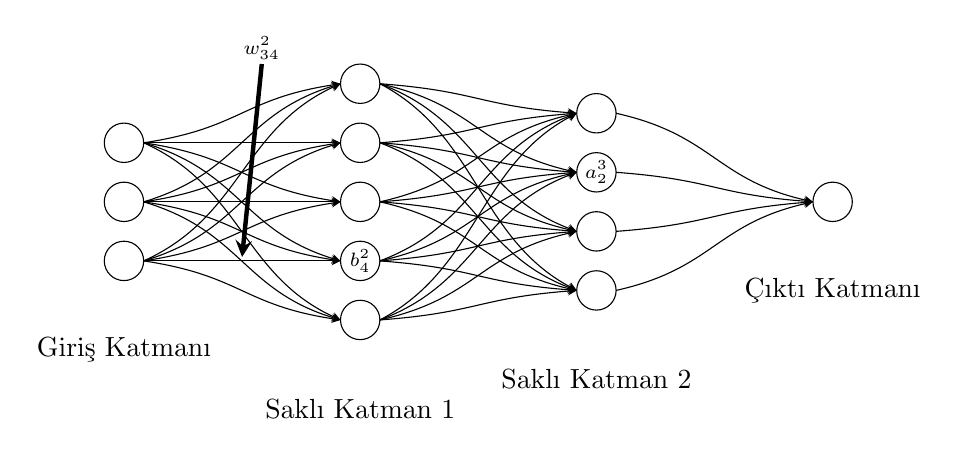
\begin{tikzpicture}[
    neuron/.style={circle, draw, minimum size=0.5cm, inner sep=0},
    arrow/.style={->, thick},
    align=center
    ]


    % Base coordinates
    \def\layers{3, 5, 4, 1} % Example: 3 input, 4 hidden, 3 hidden, 1 output
    \def\labels{Giriş Katmanı, Saklı Katman 1, Saklı Katman 2, Çıktı Katmanı}
    \def\features{}
    \def\xstart{0}    % X-coordinate for the first layer
    \def\layersep{3}  % Horizontal separation between layers
    \def\ysep{0.75}    % Vertical separation between neurons
    \def\maxneuron{11} % Threshold for number of neurons to display
    \pgfmathsetmacro{\mn}{int((\maxneuron-1)/2)}
    \pgfmathsetmacro{\ys}{int((\maxneuron+1)/2)}
    
    
    
    \foreach \i [count=\n from 1] in \layers {
        \ifnum\n = 1
            \foreach \feature [count=\n from 1] in \features {
                \pgfmathsetmacro{\yshift}{- (\i + 1) * \ysep / 2}
                \node[] at (-1.5, \yshift + \n*\ysep) {\feature};
            }
        \fi
    }
    
    
    % Process layers and neurons
    \foreach \i [count=\n from 1] in \layers {
        % Calculate the x-coordinate for the layer
        \pgfmathsetmacro{\xpos}{\xstart + (\n-1)*\layersep}
        
        % Draw neurons for the current layer and store node names in a list
        \ifnum\i > \maxneuron
            % Calculate vertical starting position for the neurons
            \pgfmathsetmacro{\yshift}{-\ys*\ysep}
            
            % Draw four neurons for the current layer
            \foreach \m in {1,2,...,\mn} {
                \pgfmathsetmacro{\t}{int(\maxneuron-\m)}
                \node[neuron] (L\n N\m) at (\xpos, \yshift + \m*\ysep) {};  % Node name L<layer> N<neuron>
                \node[neuron] (L\n N\t) at (\xpos, \m*\ysep) {};
            }
            % Add vertical ellipsis between second and third neuron
            \node at (\xpos, 0.125) {\huge$\vdots$};
        \else
            % Calculate vertical starting position for the neurons
            \pgfmathsetmacro{\yshift}{- (\i + 1) * \ysep / 2}
            
            
            % Draw all neurons for the current layer
            \foreach \m in {1,...,\i} {
                \node[neuron] (L\n N\m) at (\xpos, \yshift + \m*\ysep) {};  % Node name L<layer> N<neuron>
            }
        \fi
    }
    
    
    % Add layer labels
    \foreach \a [count=\m from 1] in \layers {
        \foreach \label [count=\n from 1] in \labels {
            \ifnum\n= \m
                \pgfmathsetmacro{\xpos}{(\n-1)*\layersep}
                \ifnum\a > \maxneuron
                    % Calculate vertical starting position for the neurons
                    \pgfmathsetmacro{\yshift}{-\maxneuron*\ysep/2}
                \else
                    % Calculate vertical starting position for the neurons
                    \pgfmathsetmacro{\yshift}{-\a*\ysep/2}
                \fi
                \node[align=center, font=\rmfamily] at (\xpos, \yshift - \ysep) {\label};
            \fi
        }
    }


    \draw[->, >=stealth, ultra thick] (\xstart + \layersep / 2 + 0.25, 2*\ysep + 0.25) -- (\xstart + 0.5*\layersep, -\ysep + 0.05);
    \node[font=\scriptsize] at (\xstart + \layersep / 2 + 0.25, 2*\ysep + 0.45) {$w^2_{34}$};
    \node[font=\scriptsize] at (\xstart + \layersep, -\ysep) {$b^2_{4}$};
    \node[font=\scriptsize] at (\xstart + 2*\layersep, \ysep/2) {$a^3_{2}$};
    
    
    % Loop through the list using pgffor
    \foreach \i [count=\n] in \layers {
        \foreach \j [count=\m] in \layers {
            \ifnum\m=\numexpr\n+1\relax
                \ifnum\i > \maxneuron
                    \pgfmathsetmacro{\ie}{\maxneuron-1}
                    \ifnum\j > \maxneuron
                        \pgfmathsetmacro{\je}{\maxneuron-1}
                        \foreach \k in {0,...,\ie} {
                            \foreach \p in {0,...,\je} {
                                \ifnum \numexpr2*\k = \ie 
                                \else
                                    \ifnum \numexpr2*\p = \je 
                                    \else
                                    \pgfmathsetmacro{\xpos}{\xstart + (\n-1)*\layersep}
                                    \pgfmathsetmacro{\yshift}{-\ys*\ysep}
                                    
                                    \pgfmathsetmacro{\nextlayer}{int(\n+1)}
                                    \draw[->, >=stealth] (\xpos + 0.25, \yshift + \k*\ysep + \ysep) .. controls (\xpos + \layersep / 2, \yshift + 3*\k*\ysep/4 + \p * \ysep / 4 + \ysep) and (\xpos + \layersep / 2, \yshift + 3*\p*\ysep / 4 + \k * \ysep / 4 + \ysep) .. (\xpos - 0.25 + \layersep, \yshift + \p*\ysep + \ysep);
                                    \fi
                                \fi
                            }
                        }
                    \else
                        \pgfmathsetmacro{\je}{\j}
                        \foreach \k in {0,...,\ie} {
                            \foreach \p in {1,...,\je} {
                                \ifnum \numexpr2*\k = \ie 
                                \else
                                \pgfmathsetmacro{\xpos}{\xstart + (\n-1)*\layersep}
                                \pgfmathsetmacro{\yshiftl}{- \ys * \ysep}
                                \pgfmathsetmacro{\yshiftr}{- (\je+1) * \ysep / 2}
                                
                                
                                \pgfmathsetmacro{\nextlayer}{int(\n+1)}
                                \draw[->, >=stealth] (\xpos + 0.25, \yshiftl + \k*\ysep + \ysep) .. controls (\xpos + \layersep / 2, 3*\yshiftl/4 + 3*\k*\ysep/4 + 3*\ysep/4 + \yshiftr/4 + \p*\ysep/4) and (\xpos + \layersep / 2, 3*\yshiftr/4 + 3*\p*\ysep/4 + \yshiftl/4 + \k*\ysep/4 + \ysep / 4) .. (\xpos - 0.25 + \layersep, \yshiftr + \p*\ysep);
                                \fi
                            }
                        }
                    \fi
                \else
                    \pgfmathsetmacro{\ie}{\i}
                    \ifnum\j > \maxneuron
                        \pgfmathsetmacro{\je}{\maxneuron-1}
                        \foreach \k in {1,...,\ie} {
                            \foreach \p in {0,...,\je} {
                                \ifnum \numexpr2*\p = \je 
                                \else
                                \pgfmathsetmacro{\xpos}{\xstart + (\n-1)*\layersep}
                                \pgfmathsetmacro{\yshiftl}{- (\ie + 1) * \ysep / 2}
                                \pgfmathsetmacro{\yshiftr}{-\ys * \ysep}
                                
                                
                                \pgfmathsetmacro{\nextlayer}{int(\n+1)}
                                \draw[->, >=stealth] (\xpos + 0.25, \yshiftl + \k*\ysep) .. controls (\xpos + \layersep / 2, 3*\yshiftl/4 + 3*\k*\ysep/4 + \yshiftr/4 + \p*\ysep/4 + \ysep/4) and (\xpos + \layersep / 2, 3*\yshiftr/4 + 3*\p*\ysep/4 + 3*\ysep/4 + \yshiftl/4 + \k*\ysep/4) .. (\xpos - 0.25 + \layersep, \yshiftr + \p*\ysep + \ysep);
                                \fi
                            }
                        }
                    \else
                        \pgfmathsetmacro{\je}{\j}
                        \foreach \k in {1,...,\ie} {
                            \foreach \p in {1,...,\je} {
                                \pgfmathsetmacro{\xpos}{\xstart + (\n-1)*\layersep}
                                \pgfmathsetmacro{\yshiftl}{- (\ie + 1) * \ysep / 2}
                                \pgfmathsetmacro{\yshiftr}{- (\je + 1) * \ysep / 2}
                                
                                \pgfmathsetmacro{\nextlayer}{int(\n+1)}
                                \draw[->, >=stealth] (\xpos + 0.25, \yshiftl + \k*\ysep) .. controls (\xpos + \layersep / 2, 3*\yshiftl/4 + 3*\k*\ysep/4 + \yshiftr/4 + \p*\ysep/4) and (\xpos + \layersep / 2, 3*\yshiftr/4 + 3*\p*\ysep/4 + \yshiftl/4 + \k*\ysep/4) .. (\xpos - 0.25 + \layersep, \yshiftr + \p*\ysep);
                            }
                        }
                    \fi
                \fi
            \fi
        }
    }
    
    
    \end{tikzpicture}
    \caption{Ağırlık, Eğilim ve Aktivasyon Bağlantılarını Vurgulayan Örnek Derin Sinir Ağı (DNN) Mimarisi}
    \label{fig:DNN_exp}
\end{figure}


\hyperref[fig:DNN_exp]{\protect\ref{fig:DNN_exp}}de, $w^2_{34}$, ikinci katmandaki dördüncü nöron ile üçüncü katmandaki ikinci nöron arasındaki bağlantının ağırlığını, $b^2_4$ ikinci katmandaki üçüncü nöronun eğilimini ve $a^3_2$ üçüncü katmandaki birinci nöronun aktivasyonunu ifade etmektedir.

Bunu daha iyi anlayabilmek için öncelikle nöronu tanımlayalım:

\begin{figure}
    \centering
    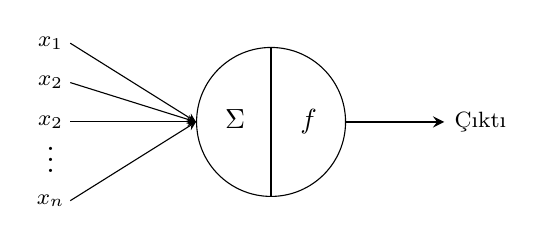
\begin{tikzpicture}[
    neuron/.style={circle, draw, minimum size=0.8cm, inner sep=0},
    input/.style={draw, -stealth},
    output/.style={draw, -stealth, thick},
    textnode/.style={align=center, font=\footnotesize}
    ]
    
    % Neuron node
    \node[neuron] (N) at (-0.2, 0) {$\hspace{1em} \Sigma \hspace{2em} f \hspace{1em}$};
    \draw[thick] (N.north) -- (N.south);
    
    % Input arrows
    \node[textnode] at (-3, 1) {$x_1$};
    \node[textnode] at (-3, 0.5) {$x_2$};
    \node[textnode] at (-3, 0) {$x_2$};
    \node at (-3, -0.375) {\large$\vdots$};
    \node[textnode] at (-3, -1) {$x_n$};
    
    \draw[input] (-2.75, 1) -- (N.west);
    \draw[input] (-2.75, 0.5) -- (N.west);
    \draw[input] (-2.75, 0) -- (N.west);
    \draw[input] (-2.75, -1) -- (N.west);
    
    
    % Output arrow
    \draw[output] (N.east) -- (2, 0) node[right, textnode] {Çıktı};
    
    \end{tikzpicture}
    \caption{Bir Nöronun Çalışma Şekli}
    \label{fig:nöron}
\end{figure}

\ref{fig:nöron}de de görüldüğü üzere bir nöronun $n\in\mathbb{N}$ adet girdi $(x_1, x_2,\dots,x_n)$ ve bir çıktısı vardır. Bu girdiler, giriş katmanından gelen verilerden veya diğer nöronların çıktılarından oluşabilir. Nöronun çıktısı, girdilerin belirli ağırlıklarla çarpılıp bir eğilim eklenerek elde edilen toplamın aktivasyon fonksiyonuna uygulanmasıyla bulunur. Matematiksel olarak bu, \eqref{eq:nöron-a} deki gibi ifade edilir \cite{nielsen2015neural}:

\begin{equation} 
    a^{l}_j = \sigma\left( \sum_k w^{l}_{jk} a^{l-1}_k + b^l_j\right)
    \label{eq:nöron-a}
\end{equation}


Teorik kısımda işlem basitliği sağlamak adına skaler çarpım işlemi $*$ operatörü ile tanımlanmıştır; yani, "x skaler çarpım y" işlemi $x * y \equiv \sum_i x_i y_i$ olarak ifade edilir. Bu tanımı kullanarak \eqref{eq:nöron-a} \eqref{eq:nöron-a-s1} e sadeleşir:
\begin{equation} 
    a^{l}_j = \sigma\left(w^l_j * a^{l-1}+b^l_j\right).
    \label{eq:nöron-a-s1}
\end{equation}

Son olarak bileşenleri $a^l_j$ aktivasyonları olan bir $a^l$ aktivasyon vektörü tanımlanır. Bu vektörü tanımlayabilmek için bir fonksiyonu özellikle aktivasyon fonksiyonunun vektörleştirilebilmesi lazım. Bir fonksiyonu vektörleştirmek, fonksiyona bir vektör verildiğinde, bu fonksiyonun vektördeki her bir bileşene ayrı ayrı uygulanması anlamına gelir. Bu tarz bir eleman yönlü (elementwise) işlemi göstermek için $\sigma(v)$ notasyonunu kullanılır (burada v, bir vektördür). Yani, $\sigma(v)$'nin bileşenleri $\sigma(v)_j = \sigma(v_j)$'dir.  Örnek olarak, mesela $f(x)=2\cdot x$ fonksiyonunun vektörleştirilmiş halinin $v=\left[ \begin{array}{c} 2 \\ 3 \end{array} \right]$ ye \eqref{eq:f_vector} de uygulandığı varsayılsın.
\begin{equation}
    f\left(\left[ \begin{array}{c} 2 \\ 3 \end{array} \right] \right)
        = \left[ \begin{array}{c} f(2) \\ f(3) \end{array} \right]
        = \left[ \begin{array}{c} 4 \\ 6 \end{array} \right]
        \label{eq:f_vector}
\end{equation}
Vektörleştirilmiş $f$ fonksiyonu her bir elemanın 2 katını almış olur. Bunu göz önünde bulundurarak \eqref{eq:nöron-a-s1} \eqref{eq:a^l} e değiştirilir:
\begin{equation}
    a^{l} = \sigma\left(W^l a^{l-1}+b^l\right)
    \label{eq:a^l}
\end{equation}
Ara bir değer olarak $z^l \equiv W^l a^{l-1} + b^l$ tanımlansın. Burada, $z^l_j$'nin bileşenlerinin $z^l_j \equiv w^l_j * a^{l-1} + b^l_j$ şeklindedir. Bu değer, maliyet fonksiyonunun gradyanını hesaplarken yararlı olacaktır.

Yani sonuç olarak sinir ağının son katmanının diğer bir deyişle çıktısının son hali \eqref{eq:a^l_z} deki gibi gösterilir:
\begin{equation} 
    a^{l} = \sigma(z^l)
    \label{eq:a^l_z}
\end{equation}

%\includegraphics[width=\linewidth, keepaspectratio]{image8}
%\includegraphics[width=\linewidth, keepaspectratio]{image9}

%\drawNN{3, 2, 1}{Input Layer, Hidden Layer, Output Layer}{Input 1, Input 2, Input 3}{2}{0.75}{11}

\subsubsection{CDAE Özellikleri}

DNN yapısının temel bileşenleri tanıtıldıktan sonra, bu yapının konvolüsyonel katmanlarla genişletilmiş hali olan CDAE mimarisi aşağıda açıklanmıştır.

Konvolüsyonel Gürültü Giderici Otokodlayıcı (CDAE) ağları, özellikle bozulmuş veya gürültülenmiş verilerin temiz halini yeniden oluşturmaya yönelik olarak tasarlanmış özel bir sinir ağı türüdür. Bu mimaride hem konvolüsyonel katmanlar hem de otokodlayıcı yapısı birlikte kullanılarak hem mekânsal özellikler korunur hem de sıkıştırma ve yeniden yapılandırma işlemleri gerçekleştirilir. Gürültü giderici otokodlayıcılar, giriş verisine yapay olarak eklenen bozulmaları öğrenerek bu bozulmaları telafi etmeyi amaçlar; böylece model, temel veri yapısını daha etkili bir biçimde öğrenir.

Özetle, klasik DNN'lar genel amaçlı öğrenme görevlerine yönelirken, CDAE'lar belirli bir görev olan gürültü azaltma ve girişin temiz halini yeniden oluşturma üzerine özelleşmiştir. Ayrıca, konvolüsyonel yapının dahil edilmesi, özellikle görüntü verilerinde, yerel bağıntıların ve mekânsal örüntülerin daha etkili biçimde yakalanmasını sağlar.


\subsection{Toplu Normalleştirme}

Toplu Normalleştirme, derin sinir ağlarının eğitimini iyileştirmek amacıyla her katmana gelen girdileri normalize eden bir tekniktir. Bu yöntem, her kanal için mini-toplu verisini tüm gözlemler boyunca normalize ederek çalışır; bu da eğitimi hızlandırır ve kararlılığı artırır.

Katman, aktivasyonları önce mevcut mini-toplu üzerinde hesaplanan ortalama çıkarılarak ve standart sapmaya bölünerek normalize eder. Bu işlem, eğitim sırasında katman girişlerinin dağılımının değişmesiyle ilgili olan içsel kovaryans kayması sorunlarını hafifletmeye yardımcı olur. Her bir giriş elemanı \( x_i \) için normalizasyon \eqref{eq:batch1} deki gibi tanımlanır:

\begin{equation}
    \widehat{x}_i = \frac{x_i - \mu_B}{\sqrt{\sigma_B^2 + \epsilon}},
    \label{eq:batch1}
\end{equation}

burada \( \mu_B \) ve \( \sigma_B^2 \), mini-toplu ortalaması ve varyansı olup, \( \epsilon \) ise sayısal kararlılık için eklenen küçük bir sabittir.

Normalizasyondan sonra, veriler öğrenilebilir parametrelerle dönüştürülerek ağın temsil gücü korunur:

\begin{equation}
    y_i = \gamma \widehat{x}_i + \beta,
    \label{eq:batch2}
\end{equation}

\eqref{eq:batch2} de \( \gamma \) öğrenilebilir bir ölçek parametresi ve \( \beta \) öğrenilebilir bir kaydırma parametresidir. Bu parametreler ağın diğer ağırlıklarıyla birlikte eğitilir.

Toplu Normalleştirme, ağ boyunca gradyanların akışını iyileştirerek optimizasyon yüzeyini daha düzgün hale getirir ve daha yüksek öğrenme oranlarının kullanılmasına olanak tanır. Ayrıca, bir örneğin aktivasyonları diğer örneklere bağlı olduğundan dolayı düzenleyici bir etki gösterir; bu da seyreltme veya güçlü ağırlık cezaları gibi diğer düzenleme tekniklerine olan ihtiyacı azaltabilir.

\begin{comment}
    https://www.mathworks.com/help/deeplearning/ref/nnet.cnn.layer.batchnormalizationlayer.html
\end{comment}


\subsection{Doğrultulmuş Doğrusal Ünite (ReLU)}


Yapay zeka bağlamında  Doğrultulmuş Doğrusal Ünite (Rectified Linear Unit – ReLU), bir aktivasyon fonksiyonudur. ReLU fonksiyonu, negatif giriş değerleri için sıfır, pozitif giriş değerleri için ise girişin kendisi kadar çıktı üretmektedir. Matematiksel olarak fonksiyon \eqref{eq:relu}'da tanımlanır \cite{zhang2014improving}. 


\begin{equation}
    f(x) = 
    \begin{cases}  
    x, & x > 0 \\  
    0, & x \leq 0  
    \end{cases}
    \label{eq:relu}
\end{equation}



\subsection{Geri Yayılım (Backpropagation)}

Geri yayılım algoritması incelenmeden önce maliyet fonksiyonu üzerinde durulması gerekmektedir. Maliyet fonksiyonunun, sinir ağının çıktılarının bir fonksiyonu olarak ifade edilebileceği varsayılmaktadır. \ref{fig:DNN_Cost} te bir maliyet fonksiyonu örneği sunulmaktadır. Bu varsayım, geri yayılım algoritmasının uygulanabilmesi için temel bir ön koşul oluşturmaktadır.

\begin{figure}[H]
    \centering
    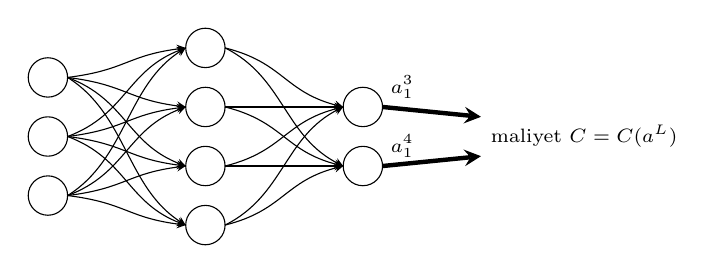
\begin{tikzpicture}[
    neuron/.style={circle, draw, minimum size=0.5cm, inner sep=0},
    arrow/.style={->, thick},
    align=center
    ]


    % Base coordinates
    \def\layers{3, 4, 2} % Example: 3 input, 4 hidden, 3 hidden, 1 output
    \def\labels{}
    \def\features{}
    \def\xstart{0}    % X-coordinate for the first layer
    \def\layersep{2}  % Horizontal separation between layers
    \def\ysep{0.75}    % Vertical separation between neurons
    \def\maxneuron{11} % Threshold for number of neurons to display
    \pgfmathsetmacro{\mn}{int((\maxneuron-1)/2)}
    \pgfmathsetmacro{\ys}{int((\maxneuron+1)/2)}
    
    
    
    \foreach \i [count=\n from 1] in \layers {
        \ifnum\n = 1
            \foreach \feature [count=\n from 1] in \features {
                \pgfmathsetmacro{\yshift}{- (\i + 1) * \ysep / 2}
                \node[] at (-1.5, \yshift + \n*\ysep) {\feature};
            }
        \fi
    }
    
    
    % Process layers and neurons
    \foreach \i [count=\n from 1] in \layers {
        % Calculate the x-coordinate for the layer
        \pgfmathsetmacro{\xpos}{\xstart + (\n-1)*\layersep}
        
        % Draw neurons for the current layer and store node names in a list
        \ifnum\i > \maxneuron
            % Calculate vertical starting position for the neurons
            \pgfmathsetmacro{\yshift}{-\ys*\ysep}
            
            % Draw four neurons for the current layer
            \foreach \m in {1,2,...,\mn} {
                \pgfmathsetmacro{\t}{int(\maxneuron-\m)}
                \node[neuron] (L\n N\m) at (\xpos, \yshift + \m*\ysep) {};  % Node name L<layer> N<neuron>
                \node[neuron] (L\n N\t) at (\xpos, \m*\ysep) {};
            }
            % Add vertical ellipsis between second and third neuron
            \node at (\xpos, 0.125) {\huge$\vdots$};
        \else
            % Calculate vertical starting position for the neurons
            \pgfmathsetmacro{\yshift}{- (\i + 1) * \ysep / 2}
            
            
            % Draw all neurons for the current layer
            \foreach \m in {1,...,\i} {
                \node[neuron] (L\n N\m) at (\xpos, \yshift + \m*\ysep) {};  % Node name L<layer> N<neuron>
            }
        \fi
    }
    
    
    % Add layer labels
    \foreach \a [count=\m from 1] in \layers {
        \foreach \label [count=\n from 1] in \labels {
            \ifnum\n= \m
                \pgfmathsetmacro{\xpos}{(\n-1)*\layersep}
                \ifnum\a > \maxneuron
                    % Calculate vertical starting position for the neurons
                    \pgfmathsetmacro{\yshift}{-\maxneuron*\ysep/2}
                \else
                    % Calculate vertical starting position for the neurons
                    \pgfmathsetmacro{\yshift}{-\a*\ysep/2}
                \fi
                \node[align=center, font=\rmfamily] at (\xpos, \yshift - \ysep) {\label};
            \fi
        }
    }


    \draw[->, >=stealth, ultra thick] (\xstart + 2*\layersep + 0.25, \ysep / 2) -- (\xstart + 2*\layersep + 1.5, \ysep/2 - 0.125);
    \draw[->, >=stealth, ultra thick] (\xstart + 2*\layersep + 0.25, -\ysep / 2) -- (\xstart + 2*\layersep + 1.5, -\ysep/2 + 0.125);
    
    \node[font=\scriptsize] at (\xstart + 2*\layersep + \ysep/2 + 0.125, \ysep/2 + 0.25) {$a^3_{1}$};
    \node[font=\scriptsize] at (\xstart + 2*\layersep + \ysep/2 + 0.125, -\ysep/2 + 0.25) {$a^4_{1}$};
    \node[font=\scriptsize, anchor=west] at (\xstart + 2*\layersep + 1.5, 0) {maliyet $C = C(a^L)$};
    
    
    % Loop through the list using pgffor
    \foreach \i [count=\n] in \layers {
        \foreach \j [count=\m] in \layers {
            \ifnum\m=\numexpr\n+1\relax
                \ifnum\i > \maxneuron
                    \pgfmathsetmacro{\ie}{\maxneuron-1}
                    \ifnum\j > \maxneuron
                        \pgfmathsetmacro{\je}{\maxneuron-1}
                        \foreach \k in {0,...,\ie} {
                            \foreach \p in {0,...,\je} {
                                \ifnum \numexpr2*\k = \ie 
                                \else
                                    \ifnum \numexpr2*\p = \je 
                                    \else
                                    \pgfmathsetmacro{\xpos}{\xstart + (\n-1)*\layersep}
                                    \pgfmathsetmacro{\yshift}{-\ys*\ysep}
                                    
                                    \pgfmathsetmacro{\nextlayer}{int(\n+1)}
                                    \draw[->, >=stealth] (\xpos + 0.25, \yshift + \k*\ysep + \ysep) .. controls (\xpos + \layersep / 2, \yshift + 3*\k*\ysep/4 + \p * \ysep / 4 + \ysep) and (\xpos + \layersep / 2, \yshift + 3*\p*\ysep / 4 + \k * \ysep / 4 + \ysep) .. (\xpos - 0.25 + \layersep, \yshift + \p*\ysep + \ysep);
                                    \fi
                                \fi
                            }
                        }
                    \else
                        \pgfmathsetmacro{\je}{\j}
                        \foreach \k in {0,...,\ie} {
                            \foreach \p in {1,...,\je} {
                                \ifnum \numexpr2*\k = \ie 
                                \else
                                \pgfmathsetmacro{\xpos}{\xstart + (\n-1)*\layersep}
                                \pgfmathsetmacro{\yshiftl}{- \ys * \ysep}
                                \pgfmathsetmacro{\yshiftr}{- (\je+1) * \ysep / 2}
                                
                                
                                \pgfmathsetmacro{\nextlayer}{int(\n+1)}
                                \draw[->, >=stealth] (\xpos + 0.25, \yshiftl + \k*\ysep + \ysep) .. controls (\xpos + \layersep / 2, 3*\yshiftl/4 + 3*\k*\ysep/4 + 3*\ysep/4 + \yshiftr/4 + \p*\ysep/4) and (\xpos + \layersep / 2, 3*\yshiftr/4 + 3*\p*\ysep/4 + \yshiftl/4 + \k*\ysep/4 + \ysep / 4) .. (\xpos - 0.25 + \layersep, \yshiftr + \p*\ysep);
                                \fi
                            }
                        }
                    \fi
                \else
                    \pgfmathsetmacro{\ie}{\i}
                    \ifnum\j > \maxneuron
                        \pgfmathsetmacro{\je}{\maxneuron-1}
                        \foreach \k in {1,...,\ie} {
                            \foreach \p in {0,...,\je} {
                                \ifnum \numexpr2*\p = \je 
                                \else
                                \pgfmathsetmacro{\xpos}{\xstart + (\n-1)*\layersep}
                                \pgfmathsetmacro{\yshiftl}{- (\ie + 1) * \ysep / 2}
                                \pgfmathsetmacro{\yshiftr}{-\ys * \ysep}
                                
                                
                                \pgfmathsetmacro{\nextlayer}{int(\n+1)}
                                \draw[->, >=stealth] (\xpos + 0.25, \yshiftl + \k*\ysep) .. controls (\xpos + \layersep / 2, 3*\yshiftl/4 + 3*\k*\ysep/4 + \yshiftr/4 + \p*\ysep/4 + \ysep/4) and (\xpos + \layersep / 2, 3*\yshiftr/4 + 3*\p*\ysep/4 + 3*\ysep/4 + \yshiftl/4 + \k*\ysep/4) .. (\xpos - 0.25 + \layersep, \yshiftr + \p*\ysep + \ysep);
                                \fi
                            }
                        }
                    \else
                        \pgfmathsetmacro{\je}{\j}
                        \foreach \k in {1,...,\ie} {
                            \foreach \p in {1,...,\je} {
                                \pgfmathsetmacro{\xpos}{\xstart + (\n-1)*\layersep}
                                \pgfmathsetmacro{\yshiftl}{- (\ie + 1) * \ysep / 2}
                                \pgfmathsetmacro{\yshiftr}{- (\je + 1) * \ysep / 2}
                                
                                \pgfmathsetmacro{\nextlayer}{int(\n+1)}
                                \draw[->, >=stealth] (\xpos + 0.25, \yshiftl + \k*\ysep) .. controls (\xpos + \layersep / 2, 3*\yshiftl/4 + 3*\k*\ysep/4 + \yshiftr/4 + \p*\ysep/4) and (\xpos + \layersep / 2, 3*\yshiftr/4 + 3*\p*\ysep/4 + \yshiftl/4 + \k*\ysep/4) .. (\xpos - 0.25 + \layersep, \yshiftr + \p*\ysep);
                            }
                        }
                    \fi
                \fi
            \fi
        }
    }
    
    
    \end{tikzpicture}
    \caption{Maliyet Fonksiyonu}
    \label{fig:DNN_Cost}
\end{figure}

İkinci dereceden maliyet fonksiyonu bu şartı sağlar, çünkü maliyet fonksiyonu \eqref{eq:cost_example} deki gibi ifade edilebilir. \begin{equation} C = \frac{1}{2} |y-a^L|^2 = \frac{1}{2} \sum_j (y_j-a^L_j)^2 \label{eq:cost_example} \end{equation} Bu durumda, maliyet fonksiyonu ağın çıktılarının bir fonksiyonu olarak yazılabilir. Bu tür bir maliyet fonksiyonu, ağın ağırlıklarının güncellenmesi için gerekli olan gradyanların hesaplanmasını mümkün kılar. Geri yayılım algoritması, gradyanları vektör toplama, bir vektörü bir matrisle çarpma gibi temel lineer cebir operatörleri kullanarak hesaplar. Ancak, bu operatörlerden biri daha nadir olarak kullanılır; bu operatör Hadamard Çarpımı'dır \cite{nielsen2015neural}.

\subsubsection{Hadamard Çarpımı \(\mathbf{\left( s \odot t \right)}\)}

Varsayalım ki s ve t aynı boyuta sahip iki vektör. O zaman bu iki vektörün eleman yönlü çarpımını göstermek için $s \odot t$ kullanılır. Burada, $s \odot t$ nin bileşenleri $\left(s \odot t\right)_j=s_jt_j$ şeklinde tanımlanır. Bu tezde, bu çarpma işlemi için Hadamard çarpımı terimi kullanılacaktır \cite{nielsen2015neural}.

\subsubsection{Geri Yayılımdaki Dört Temel Denklem}

Geri yayılım, bir ağdaki ağırlıkları ve eğilimleri değiştirmek için maliyet fonksiyonunun gradyanını kullanır. İlk olarak hata $\delta^l_j$ tanımlanır.

Hata $\delta^l_j$ \eqref{eq:error} deki gibi ifade edilir.
\begin{equation}
    \delta^l_j \equiv \frac{\partial C}{\partial z^l_j}
    \label{eq:error}
\end{equation}

\eqref{eq:error} zincir kuralı kullanılarak şu şekilde yazılabilir:
\begin{equation}
    \begin{split}
        \delta^L_j = \frac{\partial C}{\partial z^L_j} &= \frac{\partial C}{\partial a^L_j}\frac{\partial a^L_j}{\partial z^L_j} \\ &= \frac{\partial C}{\partial a^L_j}\frac{\partial \sigma}{\partial z^L_j} \left( z^L_j \right) \\ &= \frac{\partial C}{\partial a^L_j} \sigma'(z^L_j)
    \end{split}
    \label{eq:error-s}
\end{equation}

\eqref{eq:error-s} hata $\delta^L$ için eleman yönlü bir ifadedir. Fakat geri yayılım için matris formundaki hali lazımdır. \eqref{eq:error-s} i tekrar matris formunda yazarsak:
\begin{equation}
    \delta^L = \nabla_a C \odot \sigma'(z^L)
    \label{eq:error-v}
\end{equation}
\eqref{eq:error-v} de $\nabla_a C$ bileşenleri kısmi türevler $\partial C / \partial a^L_j$ olan bir vektördür.
Bu hata $\delta^l$ yi bir sonraki katmana göre hesaplanabilir.
\begin{equation}
    \delta^l = \left((W^{l+1})^T \delta^{l+1} \right) \odot \sigma'(z^l)
    \label{eq:error-r}
\end{equation}


\eqref{eq:error-r} de $(W^{l+1})^T$ $(l+1)$'nci katmanın ağırlık matrisinin devriğidir.
\eqref{eq:error-v-p} aşağıdaki şekilde çıkarılabilir:
\begin{equation}
    \begin{split}
        \delta^l_j &= \frac{\partial C}{\partial z^l_j} \\
                                &= \sum_k \frac{\partial C}{\partial z^{l+1}_k} \frac{\partial z^{l+1}_k}{\partial z^l_j} \\ 
                                &= \sum_k \delta^{l+1}_k \frac{\partial}{\partial z^l_j}  \left( \sum_i w^{l+1}_{ki} \sigma(z^l_i) +b^{l+1}_k \right) \\
                                &= \sum_k w^{l+1}_{kj}  \delta^{l+1}_k \sigma'(z^l_j) \\
                                &= \left( \hat{w}^{l+1}_j * \delta^{l+1} \right)_j \sigma'(z^l_j) \\
                                &=  (W^{l+1})^T \delta^{l+1} \odot \sigma'(z^l_j)
    \end{split}
    \label{eq:error-v-p}
\end{equation}

\eqref{eq:error-v} ile \eqref{eq:error-r} i birleştirerek, ağdaki herhangi bir katman için hata $\delta^l$'i hesaplanabilir.

Artık maliyet fonksiyonunun herhangi bir ağırlığa veya yanlılığa göre gradyanı hesaplanabilir. Maliyet fonksiyonunun gradyanı herhangi bir ağırlığa veya yanlılığa göre \eqref{eq:weight_bias} deki gibi hesaplanır \cite{nielsen2015neural}. 

\begin{equation}
    \label{eq:weight_bias}
    \begin{split}
        \frac{\partial C}{\partial w^l_{jk}} &= \frac{\partial C}{\partial z^l_j}\frac{\partial z^l_j}{\partial w^l_{jk}} \\ 
        &= \delta^l_j \frac{\partial}{\partial w^l_{jk}}\left( \sum_i w^l_{ji}a^{l-1}_i + b^l_i \right) \\ 
        &= \delta^l_j a^{l-1}_k
    \end{split}
    \qquad
    \begin{split}
        \frac{\partial C}{\partial b^l_j} &=  \frac{\partial C}{\partial z^l_j}\frac{\partial z^l_j}{\partial b^l_j} \\ 
        &= \delta^l_j \frac{\partial}{\partial b^l_j}\left( w^l_j * a^{l-1}_j + b^l_j \right) \\ 
        &= \delta^l_j
    \end{split}
\end{equation}



\begin{table}[H]
\centering
\renewcommand{\arraystretch}{2}
\begin{tabular}{|lr|}
\hline
\multicolumn{2}{|c|}{\textbf{Özet: Geri Yayılım Denklemleri}} \\
$\delta^L = \nabla_a C \odot \sigma^{\prime}\left(z^L\right)$ & \eqref{eq:error-v}\\
$\delta^l = \left( \left(W^{l+1}\right)^T \delta^{l+1} \right) \odot \sigma^{\prime}\left(z^l\right)$ & \eqref{eq:error-r} \\
$\frac{\partial C}{\partial b_j^l} = \delta_j^l$ & \eqref{eq:weight_bias} \\
$\frac{\partial C}{\partial w_{jk}^l} = a_k^{l-1} \delta_j^l$ & \eqref{eq:weight_bias} \\
\hline
\end{tabular}
\end{table}

\subsubsection{Geri Yayılım Algoritması}

Geri yayılım algoritması aşağıdaki gibidir:

\begin{itemize}
    \item \textbf{Girdi x:} Giriş katmanına karşılık gelen aktivasyon $a^1$ i tanımlanır.
    \item \textbf{İleri Besleme:} Her $l = 2, 3, \ldots, L$ için $z^l=w^la^{l-1}+b^l$ ve $a^l=\sigma(z^l)$ hesaplanır.
    \item \textbf{Çıktı Hatası $\delta^L$:} $\delta^{L} = \nabla_a C \odot \sigma'(z^L)$ vektörü hesaplanır.
    \item \textbf{Hatayı geri yay:} Her $l=L-1,L-2,\ldots,2$ için $\delta^l=((W^{l+1})^T \delta^{l+1}) \odot \sigma'(z^{l})$ hesaplanır.
    \item \textbf{Çıktı:} Maliyet fonksiyonunun gradyanı $\frac{\partial C}{\partial w^l_{jk}} = a^{l-1}_k \delta^l_j$ ve $\frac{\partial C}{\partial b^l_j} = \delta^l_j$ ile bulunmuş olur \cite{nielsen2015neural}.
\end{itemize}

\subsection{Rastgele Gradyan İnişi (SGD)}

Rastgele gradyan inişinde, gerçek gradyanı, tek bir örnekteki gradyan ile yaklaşık olarak hesaplanır ve her $l = L, L-1, \ldots, 2$ için ağırlıklar $w^l \rightarrow w^l-\eta \cdot \delta^l (a^{l-1})^T$ kuralına göre ve eğilimler $b^l \rightarrow b^l-\eta \cdot \delta^l$ kuralına göre güncellenir \cite{StochasticLeon}.


\subsection{Adam optimize edici}

Adam (Adaptive Moment Estimation), rastgele gradyan inişi (SGD) yönteminin bir çeşididir. Yöntem, gradyanların birinci ve ikinci momentlerinin kestirimlerinden farklı parametreler için bireysel uyarlanabilir öğrenme oranlarını hesaplar.

\textbf{Algoritma:}

Algoritma, gradyanın (\(m_t\)) ve kareli gradyanın (\(v_t\)) üssel hareketli ortalamalarını günceller. Burada \(\beta_1, \beta_2 \in [0, 1)\) hiperparametreleri bu değerlerin üstel azalma oranlarını belirler. Hareketli ortalamalar, gradyanın 1. anının (ortalama) ve 2. ham anının (merkezlenmemiş varyans) kestirimleridir.


Algoritmanın işleyişi aşağıda detaylı olarak adım adım açıklanmıştır:
\begin{enumerate}
    \item \textbf{Başlatma:}
    \begin{itemize}
        \item $m_0 \gets 0$: 1. moment vektörü (ortalama) sıfırla başlatılır.
        \item $v_0 \gets 0$: 2. moment vektörü (varyans) sıfırla başlatılır.
        \item $t \gets 0$: Zaman adımı 0 olarak ayarlanır.
    \end{itemize}
    
    \item \textbf{Döngü:} Algoritma, parametre $\theta_t$ yakınsamaya ulaşana kadar şu adımları tekrarlar:
    \begin{enumerate}
        \item \textbf{Gradyan Hesaplama:}
        \begin{equation}
        g_t \gets \nabla_\theta f_t(\theta_{t-1})
        \label{eq:gt}
        \end{equation}
        \eqref{eq:gt} de $t$ adımındaki stokastik hedef fonksiyonun gradyanı hesaplanır.
        
        \item \textbf{1. Moment Güncelleme:}
        \begin{equation}
        m_t \gets \beta_1 \cdot m_{t-1} + (1 - \beta_1) \cdot g_t
        \label{eq:mt}
        \end{equation}
        \eqref{eq:mt} önceki moment ($m_{t-1}$) ile yeni gradyanı ($g_t$) birleştirerek hareketli bir ortalama oluşturur.
        
        \item \textbf{2. Moment Güncelleme:}
        \begin{equation}
        v_t \gets \beta_2 \cdot v_{t-1} + (1 - \beta_2) \cdot g_t^2
        \label{eq:vt}
        \end{equation}
        \eqref{eq:vt} gradyanın karesini alarak değişkenlik (varyans) kestirimi yapar.
        
        \item \textbf{Eğilim Düzeltilmesi:}
        \begin{itemize}
            \item 1. moment için:
            \begin{equation}
            \hat{m}_t \gets \frac{m_t}{1 - \beta_1^t}
            \label{eq:mt_h}
            \end{equation}
            \eqref{eq:mt_h} moment kestirmesinin başlangıçtaki sıfır durumundan kaynaklanan eğilimi giderir.
            \item 2. moment için:
            \begin{equation}
            \hat{v}_t \gets \frac{v_t}{1 - \beta_2^t}
            \label{eq:vt_h}
            \end{equation}
            Benzer şekilde \eqref{eq:vt_h} de, 2. moment kestirmesi düzeltilir.
        \end{itemize}
        
        \item \textbf{Parametre Güncelleme:}
        \begin{equation}
        \theta_t \gets \theta_{t-1} - \alpha \cdot \frac{\hat{m}_t}{\sqrt{\hat{v}_t} + \epsilon}
        \label{eq:theta_t}
        \end{equation}
        \eqref{eq:theta_t} de $\epsilon$, sıfıra bölme hatasını önlemek için kullanılan küçük bir sabittir (örneğin, $10^{-8}$).
    \end{enumerate}
    
    \item \textbf{Sonuç:} Algoritma, yakınsama sağlandığında $\theta_t$ değerini döndürür \cite{kingma2017adammethodstochasticoptimization}.
\end{enumerate}


Algoritması, sözde kod olarak, \cite{kingma2017adammethodstochasticoptimization} makalesinden alınmıştır ve \ref{fig:adamalg}'de gösterildiği şekilde bulunabilir.

\subsubsection{L2 Düzenlemesi}

Ağırlıklar için $E(\theta)$ kayıp fonksiyonuna bir düzenleme terimi ekleyerek, aşırı öğrenmeyi azaltır \cite{PaterrecogBishop, machinelearning:2012}. Düzenleme terimine ağırlık azalması da denir. Düzenleme terimine sahip kayıp fonksiyonu \eqref{eq:L2} deki gibidir:

\begin{equation}
    E_R(\theta)=E(\theta)+\lambda \Omega(w)
    \label{eq:L2}
\end{equation}

\eqref{eq:L2} de $w$ ağırlık vektörüdür, $\lambda$ düzenleme faktörüdür (katsayı) ve düzenleme fonksiyonu $\Omega(w)$ \eqref{eq:düzenleme} deki gibidir:

\begin{equation}
    \Omega(w)=\frac{1}{2} w^T w
    \label{eq:düzenleme}
\end{equation}

Eğilimler düzenlenmez \cite{machinelearning:2012}.

\begin{figure}[H]
    \centering
    \includegraphics[width=\linewidth]{image17}
    \caption{Adam Algoritması Sözde Kodu}
    \label{fig:adamalg}
\end{figure}

\subsubsection{Gradyan Kırpma}

Gradyanların büyüklükleri üssel olarak artarsa, eğitim kararsızlaşır ve birkaç yineleme içinde farklılaşabilir. Bu "gradyan patlaması", NaN veya Inf'e giden bir eğitim kaybı demektir. Gradyan kırpma, eğitimi daha yüksek öğrenme oranlarında ve aykırı değerlerin olduğu durumlarda sabitleyerek gradyan patlamasını önlemeye yardımcı olur \cite{trainrecneural}. Gradyan kırpma, ağların daha hızlı eğitilmesini sağlar ve genellikle öğrenilen görevin doğruluğunu etkilemez.

İki tür gradyan kırpma vardır.
\begin{itemize}
\item Vektör büyüklüğü tabanlı gradyan kırpma, gradyanı bir eşik değerine göre yeniden ölçeklendirir ve gradyanın yönünü değiştirmez.
\item Değer tabanlı gradyan kırpma, eşikten büyük olan herhangi bir kısmi türevi keser ve bu da gradyanın keyfi olarak yön değiştirmesine neden olabilir. Değer tabanlı gradyan kırpma öngörülemeyen bir davranışa sahip olabilir, ancak yeterince küçük değişiklikler ağın ıraksamasına neden olmaz.
\end{itemize}

\begin{comment}
2. Text 2 ile Karşılaştırma: Eksik, Yarım veya Var mı?
Kısım	Text 2’de Anlatım Durumu	Açıklama / Önerilen Başlıklar
Veri Girişi ve Yapısı	Yarım veya eksik	Model giriş verisinin iki LDR’den 500’er ölçüm olarak birleştirildiği net değil. Burada mutlaka "Veri Seti ve Ön İşleme" başlığı altında açıklanmalı. Özellikle 1000 boyutlu vektör yapısı detaylandırılmalı.
Z-score Normalizasyon	Muhtemelen yok veya yetersiz	Veri normalizasyonun neden gerekli olduğu ve nasıl yapıldığı anlatılmalı. "Veri Ön İşleme" altında yer almalı.
Veri Bölme (Train-Val)	Yarım veya muhtemelen eksik	Veri bölme ve validasyon stratejisi net açıklanmalı. "Veri Seti Hazırlığı" veya "Model Eğitimi İçin Veri Hazırlığı" altında işlenmeli.
Veri Artırma (augmentData)	Büyük ihtimalle yok	Özellikle SNR tabanlı gürültü eklenmesi detaylandırılmalı, gerekçeleri anlatılmalı. "Veri Artırma ve Gürültü Modellenmesi" başlığı açılabilir.
Model Mimarisi (Autoencoder)	Yarım veya eksik	Text 2’de klasik DNN varken Text 3’de konvolüsyonel denoising autoencoder var. Bu önemli değişiklik "Model Mimarisi" başlığı altında açık ve detaylı anlatılmalı. Katmanlar, kernel boyutları, dropout, batch norm gibi teknik detaylar burada yer almalı.
Eğitim Parametreleri ve Metodoloji	Yarım veya eksik	Öğrenme hızı, epoch sayısı, erken durdurma, optimizasyon ayarları vb. ayrıntılı şekilde "Model Eğitimi" başlığı altında yer almalı.
Rekonstrüksiyon Hatası ve Eşik Belirleme	Eksik veya yok	Model çıktılarının değerlendirilmesi, hata hesaplaması, eşik belirleme metodolojisi "Model Değerlendirmesi" başlığında yer almalı.
Embedding Çıkarımı ve Kümeleme	Muhtemelen yok veya eksik	Özellikle "Anomali Tespiti İçin Özellik Çıkarımı ve Kümeleme" gibi bir başlık açılarak embedding çıkarmanın mantığı, k-means uygulaması, etiket eşleştirme detaylandırılmalı.
Hungarian Algoritması ile Etiket Eşleme	Büyük ihtimalle yok	Karmaşık kümeleme sonrası etiket eşleştirme yöntemi yeni ve önemli, ayrı alt başlıkta veya "Kümeleme Sonrası İşlemler" kısmında açıklanmalı.
Kod ve Fonksiyon Detayları	Metin olarak büyük ihtimalle yok	Kod doğrudan konmaz ama önemli fonksiyonların mantığı (augmentData, munkres) açıklanmalı ve gerekirse Ekler’de kod verilebilir.

3. Önerilen Başlıklar ve Alt Başlıklar (Text 3 Kapsamında)
Veri Seti ve Ön İşleme

Veri yapısı (LDR1 ve LDR2 verilerinin birleşimi)

Normalizasyon (Z-score)

Eğitim ve validasyon setine bölme

Veri artırma ve gürültü ekleme

Model Mimarisi

Konvolüsyonel Denoising Autoencoder Yapısı

Encoder ve Decoder katmanları

Latent boyutlar ve bottleneck katmanı

Model Eğitimi

Eğitim parametreleri (Epoch, batch size, öğrenme hızı)

Optimizasyon ve erken durdurma stratejileri

Performans metrikleri (RMSE)

Model Değerlendirmesi ve Anomali Tespiti

Rekonstrüksiyon hatası hesaplama ve eşik belirleme

Encoder’dan embedding çıkarımı

Kümeleme ve Sınıflandırma

K-means algoritması ile embedding kümeleme

Küme etiketlerinin gerçek sınıflarla eşleştirilmesi

Hungarian algoritması ile çakışmaların çözümü

Sonuçlar ve Kaydetme

Model çıktılarının kaydedilmesi ve ileri analiz

\end{comment}




\begin{comment}
sequenceIntputLayer

convolution1dLayer

fullyConnectedLayer ? (teoride zaten eklemiş olabiliriz emin değilim)

transposedConv1dLayer

batchNormalizationLayer

reluLayer (LReluLayer var buna benzer tanımını biraz değiştir yeterli)

dropoutLayer

rms error




\end{comment}

\begin{comment}
power (sinyal gücü)

dots (cross correlation (sinyal korelasyon gücü))




kmeans algorithm

pca (principal component analysis)

Hungarian algorithm 

percentile

\end{comment}

\subsection{Kosinüs Benzerliği ve Kosinüs Farkı}
Veri analizinde, kosinüs benzerliği, iç çarpım uzayında tanımlanmış iki sıfır olmayan vektör arasındaki benzerliği ölçen bir ölçüdür. Kosinüs benzerliği, bu vektörler arasındaki açının kosinüsüdür; yani, vektörlerin noktasal çarpımının, vektörlerin uzunluklarının çarpımına bölünmesidir. Bu nedenle, kosinüs benzerliği vektörlerin büyüklüklerine değil, yalnızca aralarındaki açıya bağlıdır. Kosinüs benzerliği daima [ -1, +1] aralığında yer alır. Kosinüs benzerliğinin formülü \eqref{eq:cosine_similarity}'da verilmiştir.


% Requires: \usepackage{amsmath}

\begin{equation}
   S_C(A, B) := \cos(\theta) = \frac{\mathbf{A} \cdot \mathbf{B}}{\|\mathbf{A}\| \|\mathbf{B}\|} = \frac{\sum_{i=1}^{n} A_i B_i}{\sqrt{\sum_{i=1}^{n} A_i^2} \cdot \sqrt{\sum_{i=1}^{n} B_i^2}}
   \label{eq:cosine_similarity}
\end{equation}

Kosinüs farkı, kosinüs benzerliği aracılığı ile bulunur. Kosinüs farkı formülü \eqref{eq:1}'da verilmiştir. 

\begin{equation}
    D_C(A, B) := 1 - S_C(A, B)
    \label{eq:1}
\end{equation}


\begin{comment}
    kaynak : Singhal, Amit (2001). "Modern Information Retrieval: A Brief Overview". Bulletin of the IEEE Computer Society Technical Committee on Data Engineering 24 (4): 35–43
\end{comment}


\subsection{Ortalama Kare Hatası (Mean Square Error - MSE )}
 
Ortalama Kare Hatası bir istatistiksel modelin tahmin ettiği değerlerle gerçek değerler arasındaki ortalama farkı ifade eder. Matematiksel olarak, artıkların (residual) standart sapmasıdır. Artıklar, regresyon doğrusu ile veri noktaları arasındaki mesafeyi temsil eder.

MSE, bu artıkların ne kadar yayıldığını nicelendirir ve gözlemlenen verilerin tahmin edilen değerlere ne kadar yakın olduğunu gösterir.

Düşük MSE değerleri, modelin veriye iyi uyum sağladığını ve daha isabetli tahminler ürettiğini gösterir. Buna karşılık, yüksek MSE değerleri daha fazla hata içerdiğini ve tahminlerin daha az hassas olduğunu ifade eder.

MSE \eqref{eq:mse} ile hesaplanılır:


\begin{equation}
    \text{MSE} = { \frac{1}{n} \sum_{i=1}^{n} (y_i - \hat{y}_i)^2 }
    \label{eq:mse}
\end{equation}
 
\subsection{Pearson Korelasyon Katsayısı (PCC)}

İlgilendiğimiz büyüklük sürekli olduğunda, iki ölçüm yöntemi veya cihazı arasındaki ilişkiyi/korelasyonu ölçmek için Pearson korelasyon katsayısı kullanılabilir. Pearson korelasyon katsayısı, iki rastgele değişken arasındaki doğrusal ilişkiyi ölçer. Diyelim ki elimizde çift veri var \(\left( y_{i1}, y_{i2} \right), i = 1, \ldots, n\). Pearson korelasyon katsayısı \(\hat{\rho}\) aşağıdaki \eqref{eq:pcc1} tahmin edilebilir:

\begin{equation}
    \hat{\rho} = \frac{s_{12}}{s_{1} s_{2}}
    \label{eq:pcc1}
\end{equation}

Burada \(s_{12}\), \(y_{1}\) ve \(y_{2}\) arasındaki örnek kovaryans olup \eqref{eq:pcc2} deki gibi:

\begin{equation}
    s_{12} = \frac{1}{n-1} \sum_{i=1}^{n} \left( y_{i1} - \bar{y}_{1} \right) \left( y_{i2} - \bar{y}_{2} \right)
    \label{eq:pcc2}
\end{equation}

olarak tanımlanır.

\(s_{1}^{2}\), \(y_{1}\)’in örnek varyansı olup \eqref{eq:pcc3} deki gibi:

\begin{equation}
    s_{1}^{2} = \frac{1}{n-1} \sum_{i=1}^{n} \left( y_{i1} - \bar{y}_{1} \right)^{2}
    \label{eq:pcc3}
\end{equation}


ve \(s_{2}^{2}\) ise \(y_{2}\)’nin örnek varyansı olup \eqref{eq:pcc4} deki gibi:

\begin{equation}
    s_{2}^{2} = \frac{1}{n-1} \sum_{i=1}^{n} \left( y_{i2} - \bar{y}_{2} \right)^{2}
    \label{eq:pcc4}
\end{equation}

şeklinde tanımlanır.

Ayrıca \eqref{eq:pcc5} deki değerler:


\begin{equation}
    \bar{y}_{1} = \frac{1}{n} \sum_{i=1}^{n} y_{i1} \quad \text{ve} \quad \bar{y}_{2} = \frac{1}{n} \sum_{i=1}^{n} y_{i2}
    \label{eq:pcc5}
\end{equation}


Eğer varyanslar biliniyorsa, Pearson korelasyon katsayısı \eqref{eq:pcc6} deki gibi hesaplanabilir:

\begin{equation}
    \rho = \frac{\sigma_{12}}{\sigma_{1} \sigma_{2}}
    \label{eq:pcc6}
\end{equation}


Pearson korelasyon katsayısının şu özellikleri vardır.

\begin{enumerate}
    \item \(\rho = 1\) olduğunda \(y_{1}\) ve \(y_{2}\) mükemmel pozitif, doğrusal korelasyon gösterir.
    \item \(\rho = -1\) olduğunda \(y_{1}\) ve \(y_{2}\) mükemmel negatif, doğrusal korelasyon gösterir.
    \item \(\rho = 0\) olduğunda \(y_{1}\) ve \(y_{2}\) korelasyonlu değildir. Bu, \(y_{1}\) ve \(y_{2}\)’nin bağımsız olduğu anlamına gelmez çünkü doğrusal olmayan bir ilişki olabilir.
    \item Eğer \(y_{1}\) ve \(y_{2}\) normal dağılım gösteriyorsa, \(\rho = 0\) ise bağımsız olduklarını gösterir.
\end{enumerate}

\begin{comment}
    (Choudhary ve Nagaraja, 2017):
    ((kaynak: https://www.sciencedirect.com/topics/engineering/pearsons-linear-correlation-coefficient ))
\end{comment}


\subsection{K-Means++ Algoritması}

K-Means++ algoritması, k-means kümeleme için başlangıç merkezlerini belirlemek amacıyla bir sezgisel yöntem kullanır. K-Means++ algoritması Lloyd algoritmasının çalışma süresini iyileştirir ve elde edilen son çözümün kalitesini artırır.

\medskip

K-Means++ algoritması, küme sayısının \(k\) olduğu varsayımıyla, başlangıç merkezlerini aşağıdaki şekilde seçer:

\begin{enumerate}
    \item Veri seti \( X \)'ten rastgele ve düzgün bir şekilde bir gözlem seçilir. Seçilen gözlem ilk merkezdir ve \( c_1 \) olarak gösterilir.
    
    \item Her gözlemin \( c_p \)'ye olan uzaklıkları hesaplanır. \( c_p \) ile \( m \) gözlemi arasındaki uzaklık \( d(x_m, c_p) \) olarak gösterilir.
    
    \item Bir sonraki merkez \( c_2 \), \( X \)'ten \eqref{eq:k1} deki gibi olasılıkla rastgele seçilir:
    
    \begin{equation}
        \frac{d^2(x_m, c_1)}{\sum_{j=1}^n d^2(x_j, c_1)}
        \label{eq:k1}
    \end{equation}
    
    
    \item \( j \) merkezini seçmek için:
    \begin{enumerate}
        \item Her gözlemin her merkeze olan uzaklıkları hesaplanır ve her gözlem en yakın olduğu merkeze atanır.
        
        \item \( m = 1, \dots, n \) ve \( p = 1, \dots, j - 1 \) için, \( j \) merkezi \( X \)'ten \eqref{eq:k2} deki gibi olasılıkla rastgele seçilir:
        
        \begin{equation}
            \frac{d^2(x_m, c_p)}{\sum_{\{k: x_k \in C_p\}} d^2(x_k, c_p)}
            \label{eq:k2}
        \end{equation}
        
        
        Burada \( C_p \), \( c_p \) merkezine en yakın tüm gözlemlerin kümesidir ve \( x_m \), \( C_p \)'ye aittir.
    \end{enumerate}
    
    Yani, her bir sonraki merkez, daha önce seçilmiş olan en yakın merkeze olan uzaklığıyla orantılı bir olasılıkla seçilir.
    
    \item \( k \) merkez seçilene kadar 4. adım tekrarlanır.
\end{enumerate}


\begin{comment}
    Arthur ve Vassilvitskii [1], çeşitli küme yapılandırmaları için yapılan bir simülasyon çalışmasıyla, k-means++'ın Lloyd algoritmasına kıyasla daha düşük bir küme-içi kareler toplamına (noktadan-küme-merkezine olan uzaklıkların karelerinin toplamı) daha hızlı yakınsadığını göstermiştir. 

    [1] Arthur, David, and Sergi Vassilvitskii. K-means++: The Advantages of Careful Seeding. In SODA ‘07: Proceedings of the Eighteenth Annual ACM-SIAM Symposium on Discrete Algorithms, 1027–1035. Society for Industrial and Applied Mathematics, 2007.
\end{comment}


\newpage
\section{TASARIM}

\subsection{Genel Bilgiler}

Projenin tasarımı kapı eşiklerinde kullanılmaya uygun olacak şekilde düşünülmüştür. Temel amaç kapı eşiğinden bir kişi geçtiğinde kişi ile ilgili LDR'den gelen voltaj verilerini toplamaya dayalıdır. Bir Bluetooth modülü, bir harici güç kaynağı, bir STM32H723ZG mikroişlemci kartı ve iki adet LDR sensöründen oluşmakta olan sistem bir kutu şeklinde duvara veyahut kapı eşiklerine monte edilebilecek şekilde tasarlanmıştır. \ref{fig:mickutu}de sistemin kutusu görülmektedir.


\begin{figure}[H]
    \centering
    \includegraphics[width=\linewidth]{image14}
    \caption{Sistemin Kutusu}
    \label{fig:mickutu}
\end{figure}


Projenin tasarımında en önemli husus, ışık temelli algılama yapılması nedeniyle sistemin kullanılacağı ortamların yeterli düzeyde ışıklandırmaya sahip olması gerekliliğidir. Bu amaçla projede iki adet LDR (Light Dependent Resistor) sensörü kullanılmıştır. Kişinin hareket hızının tespiti istendiğinde, en az iki sensör gerekmektedir; böylece birinci sensör ile ikinci sensör arasında geçen süre ölçülerek hız hesabı yapılabilir.

Sistem, harici bir güç kaynağı ile beslenmektedir. Bu güç kaynağı, olası enerji kesintilerinde sistemin ani şekilde kapanmasını engellemektedir ve modüler kullanım imkânı sağlamaktadır. Verilerin bilgisayara aktarılması için Bluetooth modülü kullanılmıştır. Bluetooth modülü, mikrodenetleyici ile bilgisayar arasında kablosuz haberleşmeyi sağlamaktadır.

Başlangıçta projede MSP430 mikrodenetleyici kartı tercih edilmiştir. MSP430'un haberleşme portlarına Bluetooth modülünün doğrudan entegre edilebilmesi, üzerinde kolaylıkla elektronik devreler kurulabilmesi, erişim kolaylığı ve düşük maliyeti bu tercihte etkili olmuştur. Ancak MSP430 mikrodenetleyicisinin işlem gücünün yetersiz kalması ve üzerinde yapay zeka tabanlı bir modelin çalıştırılamaması nedeniyle, daha yüksek performansa sahip olan STM32H723ZG mikrodenetleyicisi projeye entegre edilmiştir. STM32H723ZG, ARM Cortex-M7 mimarisi sayesinde yüksek hesaplama kapasitesi sunmakta ve yapay zeka algoritmalarının çalıştırılmasına olanak tanımaktadır.

Projenin akış diyagramı Şekil \ref{fig:akış}'te, MSP430 işlemcisi aracılığıyla sensörlerden veri almak ve bilgisayar üzerinde yapay zeka modelini oluşturmak amacıyla kurulan elektriksel bağlantılar  ise Şekil \ref{fig:elk_devre}'de gösterilmiştir. Projenin son safhasında modeli koşturan ve verileri dinamik olarak işleyen STM32H723ZG işlemcisinin bağlantı şeması \ref{fig:stmbaglanti}'da  verilmiştir.

\begin{figure}[H]
    \centering
    \includegraphics[width=0.75\linewidth]{stmsema.jpg}
    \caption{STM32H723 Bağlantı Şeması}
    \label{fig:stmbaglanti}
\end{figure}

\begin{figure}[H]
    \centering
    \includegraphics[width=\linewidth]{image12}
    \caption{Veri Toplama Akış Diyagramı}
    \label{fig:akış}
\end{figure}


\subsection{Boyutlandırmalar}

Proje eni 5.8 cm, boyu 8.4 cm, yükekliği 18 cm bir kutu olarak tasarlanmıştır. Kutu proje içerisinde kullanılan tüm bileşenleri kutu içerisine rahatça sığacağı bir hacimdedir; ayrıca içerideki bileşenlerin ısınmaması için havalandırma delikleri ile çözüm üretilmiştir. Havalandırma deliklerinin çapı 0.2 mm'dir. Sensörlerin içine sığacağı yuvaların çapı 0.3 mm'dir. Sensör yuvaları kutunun geçen kişiye bakan ön yüzünde bulunmaktadır. STM32H723ZG kartının boyutları 13.3 cm x 7 cm'dir. HC05 seri Bluetooth modülünün boyutları 35 mm x 15 mm'dir. 

Projenin Karadeniz Teknik Üniversitesi bitirme projeleri sunumlarında gösterilebilmesi amacıyla, harici batarya ile birlikte taşınabilir ve geçici bir tasarım kullanılmıştır. Bu geçici tasarımın boyutları, ana tasarımla yaklaşık olarak aynıdır. Geçici tasarım  \ref{fig:gecici}'de gösterilmiştir.

\begin{figure}[H]
    \centering
    \includegraphics[width=\linewidth]{image12_1}
    \caption{Yapay Zeka Koşturma Akış Diyagramı}
    \label{fig:akış2}
\end{figure}

\begin{figure}[H]
    \centering
    \includegraphics[width=0.8\linewidth]{image18}
    \caption{MSP430 Üzerinde Kurulan Elektrik Devresi}
    \label{fig:elk_devre}
\end{figure}


\subsection{Sistem Bileşenleri ve Seçimleri}

\subsubsection{MSP430F5529LP}
MSP430 Mikrokontrolcü Texas Instruments tarafından geliştirilen bir platformdur. Kendi 16-bit RISC(Reduced Instruction Set Computer) mimarisini kullanan mikrokontrolcünün düşük güç tüketimi ile verimli çalışma kapasitesi dolayısıyla sistemin harici batarya ile çalışma süresini uzatması, içerisinde bulunan 12 bitlik ADC ile voltajların dijital sinyale dönüşümünü dahili olarak gerçekleştirebilmesi, üzerine Bluetooth modülü entegre edilebilmesi tercihindeki ana unsurlar olmuştur. \ref{fig:MSP_HC05}de MSP430 mikrodenetleyicisi görülmektedir.

\begin{figure}[H]
    \centering
    \includegraphics[width=0.75\linewidth]{kutu.jpg}
    \caption{Geçici Tasarım}
    \label{fig:gecici}
\end{figure}

\subsubsection{HC05 Seri Bluetooth Modülü}
HC-05 seri Bluetooth modülü, Bluetooth 2.0 desteği sunan bir entegredir. 10 metreye kadar Bluetooth ile haberleşebilmeyi sağlar. EDR (Enhanced Data Rate) desteği sağlayan entegre, daha hızlı veri aktarımına olanak sağlar. UART haberleşme desteği sağlaması ve 3.3V besleme seviyesinde çalışması, mikrokontrolcü ile uyumunu sağlar. \ref{fig:MSP_HC05}de Bluetooth modülü görülmektedir.

\begin{figure}[H]
    \centering
    % First figure
    \begin{subfigure}{0.45\textwidth}
        \centering
        \includegraphics[angle=180, width=\textwidth]{image4x} % Replace with 
    \end{subfigure}
    \hfill
    % Second figure
    \begin{subfigure}{0.45\textwidth}
        \centering
        \includegraphics[angle=180, width=\textwidth]{image3x} % Replace with your file name
    \end{subfigure}
    \caption{MSP430F5529LP Mikrodenetleyicisi ve HC05 Seri Bluetooth Modülü}
    \label{fig:MSP_HC05}
\end{figure}



\subsubsection{LDR}

LDR (Light Dependent Resistor), ışığa duyarlı bir dirençtir. Bu bileşenin direnci, üzerine düşen ışık miktarına göre değişir. Ucuz maliyetli bir parçadır. Kutu önünden geçen kişinin ayrımını yapmak için kullanılan voltaj verilerinin elde edilmesi için kullanılır. \ref{fig:pow_ldr}de LDR görünmektedir.



\subsubsection{Harici Güç Kaynağı}
Harici Güç Kaynağı, bir enerji depolama cihazıdır. Projede lityum iyon bataryalı, 10.000 mAh kapasiteye sahip bir harici güç kaynağı kullanılmaktadır. Projenin Karadeniz Teknik Üniversitesi’ndeki sunumlarında, taşınabilirlik ve kesintisiz enerji sağlamak amacıyla sabit güç kaynakları yerine kolay taşınabilir, batarya destekli bir enerji kaynağı tercih edilmiştir. Böylece, sunum sırasında projenin kablo veya priz bağlantısına ihtiyaç duymadan her ortamda rahatlıkla çalıştırılması mümkün olmuştur.  \ref{fig:pow_ldr}de harici güç kaynağı görünmektedir.

\begin{figure}[H]
    \centering
    % First figure
    \begin{subfigure}{0.45\textwidth}
        \centering
        \includegraphics[angle=90, width=\textwidth]{image2x} % Replace with 
    \end{subfigure}
    \hfill
    % Second figure
    \begin{subfigure}{0.45\textwidth}
        \centering
        \includegraphics[width=\textwidth]{image1x} % Replace with your file name
    \end{subfigure}
    \caption{Harici Güç Kaynağı ve LDR Sensörü}
    \label{fig:pow_ldr}
\end{figure}

\subsubsection{NUCLEO-STMH723ZG}
Projede merkezi kontrol birimi olarak STM32H723ZG mikrodenetleyicisi tercih edilmiştir. Bu tercih, sistemin yüksek hesaplama gücüne olan ihtiyacı, çoklu sensör birimlerinden gelen verilerin işlenmesi, yapay zeka modeli çalıştırma gereksinimi ve geniş çevresel bağlantı desteği gibi kriterler göz önünde bulundurularak yapılmıştır. 

STM32H723ZG, STMicroelectronics tarafından geliştirilen ve ARM Cortex-M7 çekirdeğini temel alan yüksek performanslı bir mikrodenetleyicidir. 550 MHz saat frekansı, 1 MB flash belleği ve 564 KB RAM kapasitesiyle gömülü sistemlerde ileri düzey işlem yetenekleri sunar. Ayrıca bünyesinde barındırdığı 16-bit çözünürlüğe sahip ADC birimi, LDR sensörlerinden gelen analog sinyallerin hassas bir şekilde dijital verilere dönüştürülmesini mümkün kılmaktadır. UART, SPI, I2C, CAN ve USB gibi çok sayıda haberleşme birimi sayesinde modüler donanım bileşenleriyle kolay entegrasyon sağlanabilmektedir.  

STM32H7 serisi, CMSIS-NN ve TensorFlow Lite for Microcontrollers gibi kütüphanelerle uyumlu çalışarak, sistemde geliştirilen basit sınıflandırma algoritmalarının mikrodenetleyici üzerinde çalıştırılmasına imkân tanımaktadır. Bu sayede sensör verileri yalnızca toplanmakla kalmayıp, aynı zamanda mikrodenetleyici tarafından gerçek zamanlı olarak işlenip karar verici mekanizmalara dönüştürülebilmektedir.

\begin{figure}
    \centering
    \includegraphics[angle=90, width=0.45\linewidth]{image5x}
    \caption{NUCLEO-STMH723ZG}
    \label{fig:nucleo}
\end{figure}

\subsection{Uygulanan Yöntemler}


\subsubsection{Analog Değerlerin Dijitale Dönüşümü}

Dijital sistemlerde analog sinyallerin işlenebilmesi için ADC (Analog-Dijital Dönüştürücü) devreleri kullanılır. Bu projede, başlangıçta veri toplama ve model oluşturma sürecinde MSP430 mikrodenetleyicisinin dahili 12 bit SAR (Successive Approximation Register) ADC birimi kullanılmıştır. Analog-dijital dönüştürme işlemi, belirli bir gerilim aralığını seçilen ADC çözünürlüğüne göre ölçeklendirerek analog sinyalleri dijital değerlere dönüştürmeyi sağlar. Bu sayede, LDR sensörlerinden elde edilen gerilim değerleri, mikrodenetleyici tarafından işlenebilecek sayısal verilere dönüştürülmüştür. Model oluşturma süreci tamamlandıktan sonra, sistemin daha yüksek çözünürlükte ve daha hızlı karar verebilmesi amacıyla STM32H723ZG mikrodenetleyicisine geçilmiştir. STM32H723ZG'nin bünyesinde bulunan 16 bit ADC modülü sayesinde, LDR sensörlerinden gelen analog veriler daha hassas bir şekilde dijital değerlere dönüştürülmekte ve oluşturulan model doğrultusunda sistemin karar mekanizması çalıştırılmaktadır.

\subsubsection{Bluetooth 2.0 İletişim Protokolü}

Bluetooth bir kısa mesafe iletişim protokolüdür. Projede sensörlerden gelen gerilim verilerinin bilgisayara aktarımını sağlayan teknolojidir. Bluetooth kısa mesafelerde, düşük güçlerde veri aktarımı sağlamak amacıyla tasarlanmış bir protokoldür.

\subsubsection{Üstel Hareketli Ortalama (EMA) Filtreleme}

Üstel Hareketli Ortalama filtreleme zaman serisi verilerindeki gürültüyü azaltmak ve daha pürüzsüz bir sinyal elde etmek için kullanılan bir tekniktir. EMA son verilerin etkisini artırarak hızlı değişimleri daha iyi takip eder.

\subsection{Yazılımlar}

\subsubsection{MSP430 Üzerinde Çalışan Gömülü Yazılım}
Projede MSP430 işlemcisinin belleği üzerine yazılan kaynak kodları LDR sensörler üzerine düşen gerilimlerin takibi amacıyla yazılmıştır. Kodlar ANSI C dilinde yazılmış ve MSP430 işlemcisi için uygun olan CCS derleyicisiyle derlenmiştir. Gömülü kodu yazmak için öğrenciler KTÜ Elektrik-Elektronik Mühendisliği bölümü içerisinde verilen ELK2021 Mikroişlemciler dersinden olan birikimlerini kullanmanın yanı sıra Mikroişlemcinin üretici firması olan Texas Instruments şirketinin işlemciler için sunduğu resmi dökümanlardan faydalanmıştır.

\subsubsection{STM32H723ZG Üzerinde Çalışan Gömülü Yazılım}
Projede STM32H723ZG işlemcisinin belleği üzerine yazılan kaynak kodlar, yapay zeka modelinin işlemci üzerinde çalıştırılması amacıyla geliştirilmiştir. Kodlar C dilinde yazılmış ve STM32H7 serisi için uygun olan STM32CubeIDE ortamında derlenmiştir. Gömülü yazılımı oluşturmak için öğrenciler, KTÜ Elektrik-Elektronik Mühendisliği bölümü kapsamında aldıkları gömülü sistemler ve mikrodenetleyiciler derslerindeki bilgilerini kullanmış; ayrıca işlemci üreticisi STMicroelectronics'in sağladığı referans manüellerden ve yazılım kütüphanelerinden yararlanmıştır.

\subsubsection{Python Yazılım Dili}
Python programlama dili, LDR sensör verilerini Bluetooth aracılığıyla bilgisayara aktarmak için tercih edilmiştir. Bu seçimin temel nedenleri, serial kütüphanesinin veri iletimini kolaylaştırması ve NumPy ile pandas gibi kütüphanelerin verileri CSV formatına dönüştürerek yapay zeka eğitimi için MATLAB'e hazırlanmasını sağlamasıdır. Ayrıca, PyQtGraph gibi kütüphaneler de verilerin görsel olarak izlenmesinde kolaylık sunar.

\subsubsection{MATLAB Yazılım Dili}
Bu çalışmada, yapay zeka modelinin eğitimi için MATLAB yazılımı kullanılmıştır. MATLAB, geniş kapsamlı matematiksel ve mühendislik hesaplamaları destekleyen güçlü bir yazılım ortamı sunmaktadır. Model eğitimi sürecinde, MATLAB'ın Deep Learning Toolbox'ı kullanılarak yapay sinir ağı tasarlanmış ve eğitilmiştir. \ref{fig:yaz}de yazılımların akış şeması görülmektedir.

Mikrodenetleyici, LDR verilerini SAR ADC ile dijitale çevirip Bluetooth ile bilgisayara iletir. Python kodu, dijital LDR verilerini voltaja dönüştürür, EMA filtresi ve geri yönlü sonlu fark yöntemiyle işleyerek, önünden geçen kişiye ait verileri CSV dosyasına kaydeder. Matlab kodu CSV dosyasındaki verileri okuyup veriden özellikleri çıkarır, yapay zeka modelini belirler ve yapay zekayı eğitir.



\subsection{Malzeme Listesi ve Ekonomik Analiz}


\begin{table}[H]
\captionsetup{justification=raggedright, singlelinecheck=false}
\centering
\caption{Malzeme Listesi}
\begin{spreadtab}{{tabular}{|p{3cm}|p{6cm}|p{3cm}|p{1cm}|p{2cm}|}}
\hline
@ Malzemenin Adı                      & @ Kullanım Amacı  & @ Birim fiyatı (TL) & @ Adedi  & @ Fiyatı (TL)       \\ \hline
@ MSP430F5529LP                       & @ Verimli çalışması, 12-bit ADC, Bluetooth modülü entegrasyonu.      & 586.73              & 1        & 586.73              \\ \hline
@ NUCLEO-STMH723ZG                       & @ STM32H723ZG, yüksek performans (550 MHz), geniş bellek ve çoklu haberleşme desteğiyle sensör verilerini işleyip yapay zeka modellerini çalıştırabilir. 16-bit ADC ve AI uyumluluğu sayesinde gerçek zamanlı karar almayı sağlar.      & 1659.95              & 1        & 1659.95             \\ \hline
@ HC05 Seri Bluetooth Modülü          & @ 3.3V besleme seviyesinde çalışması, Bluetooth 2.0 + EDR protokolü ile çalışması,                  & 187.79              & 1        & 187.79              \\ \hline
@ LDR                                 & @ Işığa duyarlı olması sebebiyle voltaj bölücü olarak kullanarak veri çıkarmamız.                  & 6.61                   & 2        & 13.22                   \\ \hline
@ S-link IP-G10N Powerbank            & @ MSP430'u beslemesi, şebeke kesintileri esnasında sistemin devre dışı kalmasını engellemesi ve uzun çalışma süresi olması.                   & 404.91              & 1        & 404.91              \\ \hline
@ Kutu           & @ Kutunun boyutları, bileşenlerin yerleşimi ve işlevselliği için optimize edilmiştir; havalandırma delikleri ve sensör yuvaları, aşırı ısınmayı engelleyerek etkin çalışmayı sağlar.        & 200              & 1        & 200              \\ \hline
\multicolumn{4}{|l|}{@ Toplam} & sum(e2:e7) \\ \hline
\end{spreadtab}
\end{table}

\begin{figure}[H]
    \centering
    \includegraphics[width=\linewidth]{image13_1}
    \caption{Yazılım Akış Şeması}
    \label{fig:yaz}
\end{figure}

\subsection{Hukuki Boyut}
Bir projenin gerçekleştirilmesi sırasında, çeşitli hukuki sorunlarla karşılaşılabilir.

Fikri Mülkiyet Hakları: Projenin içeriğinde kullanılan yazılım, tasarım, marka veya patentler gibi fikri mülkiyet haklarının ihlali durumlarıdır. Bu, projede kullanılan materyallerin izinsiz kullanılması veya başka bir tarafından sahip olunan fikri mülkiyet haklarının ihlali anlamına gelir.

Veri Güvenliği ve Gizlilik: Projede kullanılan verilerin güvenliği ve gizliliği ile ilgili sorunlar. Özellikle kişisel verilerin korunması gerekiyorsa, bu konuda ihlaller hukuki sorunlara yol açabilir.

Hukuki süreçlerin doğru yönetilmesi, projenin başarıya ulaşmasında kritik bir rol oynayabilir.

\subsubsection{Kişisel Verileri Koruma Kanunu}

Madde 1- (1) Bu Kanunun amacı, kişisel verilerin işlenmesinde başta özel hayatın gizliliği
olmak üzere kişilerin temel hak ve özgürlüklerini korumak ve kişisel verileri işleyen gerçek ve
tüzel kişilerin yükümlülükleri ile uyacakları usul ve esasları düzenlemektir.

Madde 2- (1) Bu Kanun hükümleri, kişisel verileri işlenen gerçek kişiler ile bu verileri
tamamen veya kısmen otomatik olan ya da herhangi bir veri kayıt sisteminin parçası olmak
kaydıyla otomatik olmayan yollarla işleyen gerçek ve tüzel kişiler hakkında uygulanır.

\subsubsection{Teknoloji Geliştirme Bölge Kanunu}

Madde 1 – Bu Kanunun amacı, üniversiteler, araştırma kurum ve kuruluşları ile üretim
sektörlerinin işbirliği sağlanarak, ülke sanayisinin uluslararası rekabet edebilir ve ihracata yönelik bir yapıya kavuşturulması maksadıyla teknolojik bilgi üretmek, üründe ve üretim yöntemlerinde yenilik geliştirmek, ürün kalitesini veya standardını yükseltmek, verimliliği artırmak, üretim maliyetlerini düşürmek, teknolojik bilgiyi ticarileştirmek, teknoloji yoğun üretim ve girişimciliği desteklemek, küçük ve orta ölçekli işletmelerin yeni ve ileri teknolojilere uyumunu sağlamak, (...)\textsuperscript{\cite{kanun7263}} teknoloji yoğun alanlarda yatırım olanakları yaratmak, araştırmacı ve vasıflı kişilere iş
imkânı yaratmak, teknoloji transferine yardımcı olmak ve yüksek/ileri teknoloji sağlayacak yabancı sermayenin ülkeye girişini hızlandıracak teknolojik alt yapıyı sağlamaktır.

b) Teknoloji Geliştirme Bölgesi (Bölge): Yüksek/ileri teknoloji kullanan ya da yeni teknolojilere yönelik firmaların, belirli bir üniversite veya yüksek teknoloji enstitüsü ya da Ar-Ge merkez veya enstitüsünün olanaklarından yararlanarak teknoloji veya yazılım ürettikleri/geliştirdikleri, teknolojik bir buluşu ticari bir ürün, yöntem veya hizmet haline dönüştürmek için faaliyet gösterdikleri ve bu yolla bölgenin kalkınmasına katkıda bulundukları, aynı üniversite, yüksek teknoloji enstitüsü ya da Ar-Ge merkez veya enstitüsü alanı içinde veya yakınında; akademik, ekonomik ve sosyal yapının bütünleştiği siteyi veya bu özelliklere sahip teknoparkı, (...)\textsuperscript{\cite{kanun7263}}

\begin{comment}
Tasarım kısmında, çalışmada yapılan hesaplamalar ilgili teori ve
teoremlere dayandırılarak açıklanmak zorundadır. Yapılacak projenin
teorik altyapısına da bağlı olarak gerekli hesaplamalar ve varsa
çizimler yapılmalıdır. Hesaplamalarda kullanılan sayısal değerler
çizelgeler halinde verilmeli, hesaplama sonuçları da ya çizelge ya da
şekillerle gösterilmelidir. Tasarım çizimlerinde çizim kağıdında başlık
(antet) bulunmalı, çizimin ne zaman, kim ve kimler tarafından, kimin
danışmanlığında, hangi proje kapsamında yapıldığı bilgileri yer
almalıdır. Tasarım çizimlerinda tüm boyutlandırma ölçülerinin sayısal
olarak verilmesi zorunludur. Tasarım bölümünün sonunda yapılacak
çalışmanın tüm detayları ortaya konmalı kullanılacak ve satın alınacak
malzeme listesi çıkarılarak listelenmeli ve \textbf{ön maliyet
hesabı yapılmalıdır.} Ayrıca projenin gerçekleştirilmesi ve sonrasında
kullanılırken oluşturabileceği hukuksal sorunlar araştırılmalı ve
yazılmalıdır.

Tasarımla ilgili bölümler aşağıdaki alt başlıklara sahip olabilir.

---
config:
  layout: fixed
  fontSize: 22px
---
flowchart LR
    A["Harici Batarya"] --> B["Mikrodenetleyici"]
    C["LDR Sensörleri"] --> B
    B --> D["Bluetooth Modülü"]
    D -.-> F["Bilgisayar"]

---
config:
  layout: fixed
  fontSize: 22px
---
flowchart LR
    A["Mikrodenetleyici, LDR verilerini SAR ADC ile dijitale çevirip Bluetooth ile bilgisayara iletir."] --> B["Python kodu, dijital LDR verilerini voltaja dönüştürür, EMA filtresi ve geri yönlü sonlu fark yöntemiyle işleyerek, önünden geçen kişiye ait verileri CSV dosyasına kaydeder."]
    B --> C["Matlab kodu CSV dosyasındaki verileri okuyup veriden özellikleri çıkarır, yapay zeka modelini belirler ve yapay zekayı eğitir."]
    A@{ shape: rect}

\textbf{3.2. Boyutlandırmalar}

Kullanılacak olan masa, kutu, montaj yatağı vb. malzeme
boyutlandırmaları yapılır. İçlerine konulacak elemanların boyutları ve
ara boşlukları da dikkate alınarak kullanılacak dış kutu ve montaj
yatağı gibi kısımlar boyutlandırılır.

\textbf{3.3. Sistem Bileşenleri ve Seçimleri}

Kullanılacak olan alt sistem bileşenlerinin neler olduğu ve nasıl
seçildikleri bu ayrıtta açıklanabilir. Seçilen komponentlerin
fotograflarını vermek onların açıklanması anlamına gelmez. Unutulmamalı
ki bu yazılan rapor bir Tasarım Projesi Raporu veya bir Bitirme Projesi
Tez Kitabıdır. Ürün katoloğu değildir. Kullanılan elemanlar
fotoğraflarıyla değil, teknik özellikleri ve projede neden, nasıl
kullanıldıkları öne çıkarılarak açıklanmalıdırlar. Nasıl seçildikleri de
açıklanmalıdır.

\textbf{3.4. Uygulanan Yöntemler}

Çalışmanın değişik safhalarında uygulanan yöntemler bu ayrıtta
açıklanmalıdır. Devre tasarım yöntemleri, kontrol yöntemleri, sayısal
çözümleme yöntemleri, haberleşme yöntemleri, konuya özgü ne tür uygulama
yöntemi yarsa burada açıklanmalıdır.

\textbf{3.5. Yazılımlar}

Çalışmada yazılım geliştirilmişse bu yazılıma ait akış şeması burada
verilerek gerekli açıklamalar yapılmalıdır. Yazılımın kodunu burada
vermeyiniz. Eğer tez danışmanı öğretim üyesi yazılım kodunun mutlaka
konulmasını isterse o zaman ekler kısmına ayrı bir ek olarak
eklenebilir.

Çalışmanın simülasyonu için kullanılan paket program türü yazılım varsa
o yazılımdan da burada kısaca bahsedilebilir. Sümülasyon çalışmasını
burada anlatmayınız. Bir sonraki bölüm zaten doğrudan simülasyon
çalışmaları içindir.

\newpage

\textbf{3.6. Malzeme Listesi ve Ekonomik Analiz}

Çalışmada kullanılacak olan malzemelerin tam listesi bu ayrıtta verilir.
Çizelge 3.1 dekine benzer bir çizelge halinde malzemenin ismi, nerede
niçin kullanılacağı, birim fiyatı ve kaç addet gerektiği yazılır. Tüm
malzemelerin fiyatları toplanarak genel bütçe oluşturulur ve proje
bütçesi ile karşılaştırılır. Bütçeye uygun bir malzeme listesi
oluşturmak için ne tür değerlendirmeler ve tercihler yapıldığı da burada
açıklanır. Kullanılacak malzemelerin fiyat ve kalitesinin proje
üzerindeki olumlu ve olumsuz etkileri değerlendirilerek buraya yazılır.

Çizelge 3.1. Malzeme Listesi

\begin{longtable}[l]{@{}
  >{\raggedright\arraybackslash}p{(\columnwidth - 8\tabcolsep) * \real{0.2585}}
  >{\raggedright\arraybackslash}p{(\columnwidth - 8\tabcolsep) * \real{0.2951}}
  >{\raggedright\arraybackslash}p{(\columnwidth - 8\tabcolsep) * \real{0.1968}}
  >{\raggedright\arraybackslash}p{(\columnwidth - 8\tabcolsep) * \real{0.0984}}
  >{\raggedright\arraybackslash}p{(\columnwidth - 8\tabcolsep) * \real{0.1512}}@{}}
\begin{tabular}{|llll|l|}
\hline
\multicolumn{1}{|l|}{Malzemenin adı} & \multicolumn{1}{l|}{Kullanım amacı} & \multicolumn{1}{l|}{Birim fiyatı (TL)} & Adedi & Fiyatı (TL) \\ \hline
\multicolumn{1}{|l|}{}               & \multicolumn{1}{l|}{}               & \multicolumn{1}{l|}{}                  &       &             \\ \hline
\multicolumn{1}{|l|}{}               & \multicolumn{1}{l|}{}               & \multicolumn{1}{l|}{}                  &       &             \\ \hline
\multicolumn{1}{|l|}{}               & \multicolumn{1}{l|}{}               & \multicolumn{1}{l|}{}                  &       &             \\ \hline
\multicolumn{1}{|l|}{}               & \multicolumn{1}{l|}{}               & \multicolumn{1}{l|}{}                  &       &             \\ \hline
\multicolumn{4}{|r|}{TOPLAM}                                                                                                &             \\ \hline
\end{tabular}
\end{longtable}

\textbf{3.7. Hukuki Boyut}

Projenin konusuna bağlı olarak gerçekleştirilmesi sırasında
karşılaşılabilecek hukuki sorunlar bu başlık altında
değerlendirilmelidir. Proje tamamlandıktan sonra karşılaşılabilecek
hukuki sorunlara da burada yer verilmelidir. Proje konusu ile ilgili
yönetmeliklere ve mevzuatlara de burada yer verilir. Bu konuda
\textbf{mevzuat.gov.tr} web adresi faydalı olabilir.
\end{comment}


\begin{comment}

Yeni işlemciye geçildi. Yeni işlemcinin bağlantıları farklı olucak o yüzden bağlantı yeni bağlantı şeması lazım. boyutu farklı bu yüzden kutu tasarımı değişecek. 



\end{comment}

\newpage
\section{SİMÜLASYON ÇALIŞMALARI}


\subsection{Simulasyon Yazılımları}

Simulasyonda verilerin elde edilmesi Python yazılımı üzerinden ve verilerin işlenmesi ise MATLAB yazılımı üzerinden yapılmıştır.

\subsubsection{Verilerin Elde Edilmesi}


\textbf{Yazılımda Kullanılan Kütüphaneler}

\begin{itemize}
    \item \textbf{serial:} Seri port üzerinden haberleşme sağlayarak MSP430 mikrodenetleyicisinden gelen verileri almak için kullanılıyor.
    \item \textbf{csv:} Toplanan verileri CSV dosyasına kaydetmek için kullanılıyor.
    \item \textbf{numpy:} Matematiksel hesaplamalar için kullanılıyor.
    \item \textbf{pandas:} CSV dosyasına veri yazmak için kullanılıyor.
    \item \textbf{pyqtgraph:} MSP430'dan gelen verilerin gerçek zamanlı grafiğini çizmek için kullanılıyor.
\end{itemize}

\textbf{Yazılımın Genel İşleyişi}

Yazılım, PyQtGraph kütüphanesi kullanarak bir grafiksel kullanıcı arayüzü (GUI) oluşturur. Bu GUI'da MSP430'dan gelen seri veri akışı LDR1 ve LDR2 için hem filtrelenmemiş hem de EMA yöntemi ile filtrelenmiş olarak sırasıyla ilk 2 çizelgede gösterilir. Son çizelgede ise bu LDR1 ve LDR2 içinde geri yönde sonlu fark gösterilir. Bu sonlu fark LDR'lerin önüne geçtiğinde negatif olur ve önünden çıktığında pozitif olur. Bu negatif ve pozitif değerleri kullanarak hareketin başlangıcı ve bitişi algılanır. Sonrasında veri sabit 500 örnek olması için eğer az veri alındıysa verideki maksimum değer eklenir ya da fazla veri alındıysa eşit aralıklarda bazı veriler çıkarılır ve istenen 500 örneğe ulaşılır. Bunu yapmamızın sebebi yapay zekanın sabit bir uzunlukta veri alması gerekmesidir.

\subsubsection{Verilerin İşlenmesi ve Yapay Zekanın Eğitilmesi}

Verilerin işlenmesi ve yapay zekada eğitilmesi bir MATLAB kodu ile yapılmıştır. Yazılım, önceden kaydedilen CSV dosyalarını okuyarak LDR1 ve LDR2’ye ait her biri 500 ölçüm içeren voltaj verilerini alır ve bu verileri tek bir vektörde birleştirerek 1000 ölçüm uzunluğunda bir vektör oluşturur. Kategorisel ("engin", "taha", "idris") bir veri seti oluşturulur. Bu veri seti için bir eğitim-doğrulama ayrım oranı belirlenir ve bu orana göre eğitim ve doğrulama alt kümeleri oluşturulur. Eğitim veri seti veri setinin ortalama sinyal gücünün belirli oranlarında gürültü eklenerek modelin girdisi oluşturulur ve çıktısı orijinal veridir. Bunun sebebi modelin eklenen gürültüler sayesinde genelleme yeteneğini arttırmak. Veri seti hazırlandıktan sonra Konvolüsyonel Gürültü Giderici Otokodlayıcı (CDAE) modeli, oluşturulan veri kümesi üzerinde eğitilir.

\subsection{Sistem Modelleme}

Sistem, LDR'ler üzerinden hareket tespiti yapmak için kullanılan verilerin toplanması, işlenmesi ve yapay zeka ile analiz edilmesi sürecini kapsamaktadır. Bu süreç, Python Yazılımı ve MATLAB Yazılımı olmak üzere iki ana aşamaya ayrılmıştır ve sistem diyagramında aşağıdaki gibi gösterilmiştir.

\subsubsection{Sistem Genel Görünümü}

\begin{itemize}
    \item \textbf{MSP430 Veri Toplama:} Sistem, MSP430 mikrodenetleyicisinden LDR1 ve LDR2'den gelen gerilim verilerinin 16-Bit ADC kullanılarak dijital değerlere çevrilmiş halini Bluetooth yoluyla alır.
    \item \textbf{Python Yazılımı (Veri Görselleştirme ve Kaydetme):}
    \begin{itemize}
        \item \textbf{Ham ADC Değerlerinin Voltaja Dönüştürülmesi:} Ham 12 bitlik ADC değerleri (ch0\_raw, ch1\_raw) 4 bit sola kaydırılarak oluşturulan 16 bitlik veriler, referans voltajı (REF\_VOLTAGE = 3.3 V) ve 16 bitlik bir tam sayının maksimum değeri (UINT16\_MAX = 65535) kullanılarak voltaja ölçeklenir. Denklemi şu şekildedir: ch0\_voltage = (ch0\_raw / UINT16\_MAX) * REF\_VOLTAGE.
        
        \item \textbf{EMA ile Veri Filtreleme:} Veriler bu yöntem kullanılarak filtrelenir. Bu yöntem, verilerdeki ani dalgalanmaları düzeltir ve önemli değişiklikleri tespit etmeyi kolaylaştırır. Filtrenin matematiksel denklemi şu şekildedir:
        
        \begin{equation}
            Y_t=\alpha X_t + (1-\alpha)Y_{t-1}
            \label{eq:ema}
        \end{equation}
        
        \eqref{eq:ema} de, \(\alpha\) filtreleme katsayısı 0.05 seçilmiştir, \(X_t\) şimdiki veri noktası, \(Y_t\) şimdiki filtrelenmiş veri noktası, \(Y_{t-1}\) bir önceki filtrelenmiş veri noktasıdır.

        \item \textbf{PyQtGraph ile Gerçek Zamanlı Grafikleme:} PyQtGraph ile Gerçek Zamanlı Grafikleme: Python yazılımı, PyQtGraph kütüphanesini kullanarak bir GUI oluşturur ve gelen verilerin voltajlarını ve sonlu farklarını gerçek zamanlı olarak çizer.

        \item \textbf{Geri Yönde Sonlu Fark ile Hareket Tespiti:} Sonlu fark yaklaşımı kullanılarak hareket tespiti yapılır. Bir nesne (örneğin bir kişi) LDR'lerin önünden geçtiğinde sonlu fark değeri negatif olur. Nesne uzaklaştığında ise bu değer pozitif olur. Bu işaret değişikliği, hareketin başlangıcı ve bitişini tespit etmek için kullanılır. Matematiksel denklemi şu şekildedir:

        \begin{equation}
            \nabla_h[V](t) = V_{t-1} - V_{t-1-h}
            \label{eq:finite_diff}
        \end{equation}
        
        \eqref{eq:finite_diff} de \(h\)'ın değeri 100'dür.
        
        \item \textbf{Veri Kaydetme:} Hareket tespiti sonuçları CSV formatında kaydedilir.
    \end{itemize}
    \item \textbf{MATLAB Yazılımı (Veri İşleme ve Yapay Zeka Eğitimi):}
    \begin{itemize}
        \item \textbf{Veri Eğitim/Doğrulama Ayırma:} Veriler belirli bir oranda eğitim ve doğrulama veri kümelerine ayrılır. Bu veri setleri, yapay zekayı eğitmek için kullanılır.

        \item \textbf{}
        
        \item \textbf{DNN Eğitimi:} Bu veri kümesi üzerinde Geri Yayılım yöntemi kullanılarak bir DNN eğitilir.
        
        \item \textbf{Simülasyon Tamamlanması:} Eğitim tamamlandıktan sonra, modelin performansı değerlendirilir ve sistem simülasyonu tamamlanır.
    \end{itemize}
\end{itemize}



\subsection{Simulasyonun Gerçekleştirilmesi}

Simülasyon, verilerin toplanması ve bu verilerle yapay zekanın eğitilmesi olmak üzere iki aşamaya ayrılabilir.


\subsubsection{Verilerin Toplanması}

İlk olarak, MSP430 mikrodenetleyicisi Bluetooth aracılığıyla bilgisayara bağlanır. Bağlantı kurulduktan sonra, hareketin başlangıç ve bitiş noktalarını belirlemek amacıyla geri yönde sonlu fark yöntemi kullanan bir Python kodu çalıştırılır. Ardından, bir kişi LDR'lerin önünden defalarca geçerek veri toplama işlemi gerçekleştirilir. Toplanan veriler CSV formatında kaydedilir. Bu süreci açıklayan bir UML diyagramı \ref{fig:simulasyongerçekleştirmesi}de görülmektedir.


\begin{figure}[H]
    \centering
    \includegraphics[width=\linewidth, keepaspectratio]{image3.png}
    \caption{Simulasyon Diyagramı}
    \label{fig:simulasyongerçekleştirmesi}
\end{figure}


\ref{fig:örnekverialımı_combined}de, cihazın ve bir kişinin hareketini ve bu hareketle alınan verilerin grafiği görülmektedir.


\subsubsection{Yapay Zekanın Eğitilmesi}

Toplanan veriler MATLAB’e yüklenir. Elde edilen veri kümesi, eğitim ve doğrulama olarak ikiye ayrılır. CDAE katmanları ve eğitim seçenekleri belirlenir. Son olarak yapay zeka modeli eğitilir. CDAE mimarisi ise \ref{fig:model_temsili}de temsili olarak sunulmaktadır. CDAE mimarisinde, çok sayıda nöron bulunduğundan, görsel bütünlüğün korunabilmesi amacıyla saklı katmanlardaki her bir nöron çizilmemiştir.

\begin{figure}[H]
    \centering
    \includegraphics[width=\linewidth]{media/model_temsili.jpg}
    \caption{Modelimizin temsili mimarisi}
    \label{fig:model_temsili}
\end{figure}

\begin{figure}[H]
    \centering
    \begin{subfigure}[t]{0.49\textwidth} % Adjust the width to less than 0.5\textwidth
        \centering
        \includegraphics[width=\linewidth]{image23}
    \end{subfigure}
    \hfill % Adds horizontal space between the figures
    \begin{subfigure}[t]{0.49\textwidth} % Adjust the width to less than 0.5\textwidth
        \centering
        \includegraphics[width=\linewidth]{plot2}
    \end{subfigure}
    \caption{MSP430 ADC Verileriyle Algılanan Bir Kişinin Geçişine Ait Veriler ve Grafiği}
    \label{fig:örnekverialımı_combined}
\end{figure}




\begin{comment}

\begin{figure}[H]
    \centering
    %%\drawNN{8, 25, 50, 25, 3}{Girdi Katmanı, Saklı \\ Katman 1, Saklı \\ Katman 2, Saklı \\ Katman 3, Çıktı Katmanı}{LDR 2 Minimum, LDR 2 Maksimum, LDR 2 RMS, LDR 2 Ortalama, LDR 1 Minimum, LDR 1 Maksimum, LDR 1 RMS, LDR 1 Ortalama}{2.5}{0.75}{11}
    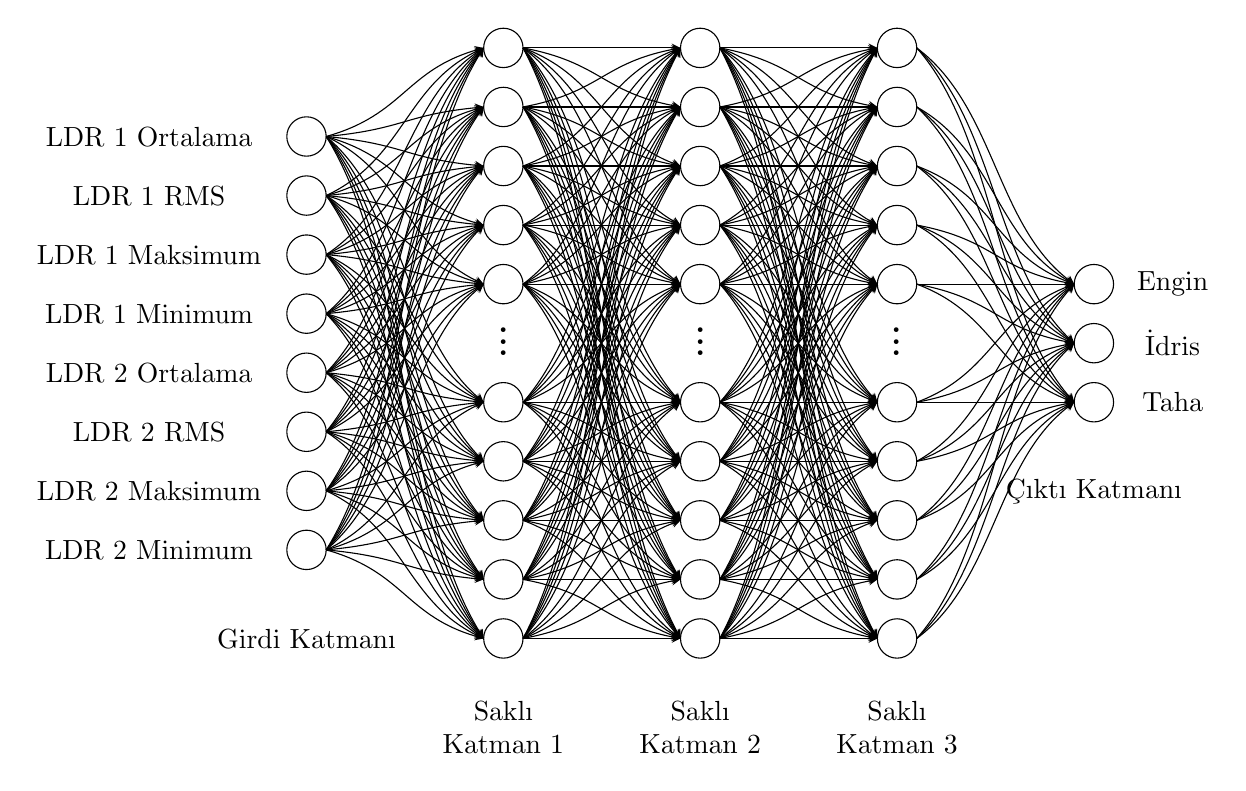
\begin{tikzpicture}[
    neuron/.style={circle, draw, minimum size=0.5cm, inner sep=0},
    arrow/.style={->, thick},
    align=center
    ]


    % Base coordinates
    \def\layers{8, 25, 50, 25, 3} % Example: 3 input, 4 hidden, 3 hidden, 1 output
    \def\labels{Girdi Katmanı, Saklı \\ Katman 1, Saklı \\ Katman 2, Saklı \\ Katman 3, Çıktı Katmanı}
    \def\features{LDR 2 Minimum, LDR 2 Maksimum, LDR 2 RMS, LDR 2 Ortalama, LDR 1 Minimum, LDR 1 Maksimum, LDR 1 RMS, LDR 1 Ortalama}
    \def\outputs{Taha, İdris, Engin}
    \def\xstart{0}    % X-coordinate for the first layer
    \def\layersep{2.5}  % Horizontal separation between layers
    \def\ysep{0.75}    % Vertical separation between neurons
    \def\maxneuron{11} % Threshold for number of neurons to display
    \pgfmathsetmacro{\mn}{int((\maxneuron-1)/2)}
    \pgfmathsetmacro{\ys}{int((\maxneuron+1)/2)}
    
    
    
    \foreach \i [count=\n from 1] in \layers {
        \ifnum\n = 1
            \foreach \feature [count=\n from 1] in \features {
                \pgfmathsetmacro{\yshift}{- (\i + 1) * \ysep / 2}
                \node[] at (-2, \yshift + \n*\ysep) {\feature};
            }
        \fi
    }

    \foreach \i [count=\n from 1] in \layers {
        \ifnum\n = 1
            \foreach \out [count=\n from 1] in \outputs {
                \pgfmathsetmacro{\yshift}{- (3 + 1) * \ysep / 2}
                \node[] at (1 + 4*\layersep, \yshift + \n*\ysep) {\out};
            }
        \fi
    }

    
    
    
    % Process layers and neurons
    \foreach \i [count=\n from 1] in \layers {
        % Calculate the x-coordinate for the layer
        \pgfmathsetmacro{\xpos}{\xstart + (\n-1)*\layersep}
        
        % Draw neurons for the current layer and store node names in a list
        \ifnum\i > \maxneuron
            % Calculate vertical starting position for the neurons
            \pgfmathsetmacro{\yshift}{-\ys*\ysep}
            
            % Draw four neurons for the current layer
            \foreach \m in {1,2,...,\mn} {
                \pgfmathsetmacro{\t}{int(\maxneuron-\m)}
                \node[neuron] (L\n N\m) at (\xpos, \yshift + \m*\ysep) {};  % Node name L<layer> N<neuron>
                \node[neuron] (L\n N\t) at (\xpos, \m*\ysep) {};
            }
            % Add vertical ellipsis between second and third neuron
            \node at (\xpos, 0.125) {\huge$\vdots$};
        \else
            % Calculate vertical starting position for the neurons
            \pgfmathsetmacro{\yshift}{- (\i + 1) * \ysep / 2}
            
            
            % Draw all neurons for the current layer
            \foreach \m in {1,...,\i} {
                \node[neuron] (L\n N\m) at (\xpos, \yshift + \m*\ysep) {};  % Node name L<layer> N<neuron>
            }
        \fi
    }
    
    
    % Add layer labels
    \foreach \a [count=\m from 1] in \layers {
        \foreach \label [count=\n from 1] in \labels {
            \ifnum\n= \m
                \pgfmathsetmacro{\xpos}{(\n-1)*\layersep}
                \ifnum\a > \maxneuron
                    % Calculate vertical starting position for the neurons
                    \pgfmathsetmacro{\yshift}{-\maxneuron*\ysep/2}
                \else
                    % Calculate vertical starting position for the neurons
                    \pgfmathsetmacro{\yshift}{-\a*\ysep/2}
                \fi
                \node[align=center, font=\rmfamily] at (\xpos, \yshift - \ysep) {\label};
            \fi
        }
    }


    
    
    % Loop through the list using pgffor
    \foreach \i [count=\n] in \layers {
        \foreach \j [count=\m] in \layers {
            \ifnum\m=\numexpr\n+1\relax
                \ifnum\i > \maxneuron
                    \pgfmathsetmacro{\ie}{\maxneuron-1}
                    \ifnum\j > \maxneuron
                        \pgfmathsetmacro{\je}{\maxneuron-1}
                        \foreach \k in {0,...,\ie} {
                            \foreach \p in {0,...,\je} {
                                \ifnum \numexpr2*\k = \ie 
                                \else
                                    \ifnum \numexpr2*\p = \je 
                                    \else
                                    \pgfmathsetmacro{\xpos}{\xstart + (\n-1)*\layersep}
                                    \pgfmathsetmacro{\yshift}{-\ys*\ysep}
                                    
                                    \pgfmathsetmacro{\nextlayer}{int(\n+1)}
                                    \draw[->, >=stealth] (\xpos + 0.25, \yshift + \k*\ysep + \ysep) .. controls (\xpos + \layersep / 2, \yshift + 3*\k*\ysep/4 + \p * \ysep / 4 + \ysep) and (\xpos + \layersep / 2, \yshift + 3*\p*\ysep / 4 + \k * \ysep / 4 + \ysep) .. (\xpos - 0.25 + \layersep, \yshift + \p*\ysep + \ysep);
                                    \fi
                                \fi
                            }
                        }
                    \else
                        \pgfmathsetmacro{\je}{\j}
                        \foreach \k in {0,...,\ie} {
                            \foreach \p in {1,...,\je} {
                                \ifnum \numexpr2*\k = \ie 
                                \else
                                \pgfmathsetmacro{\xpos}{\xstart + (\n-1)*\layersep}
                                \pgfmathsetmacro{\yshiftl}{- \ys * \ysep}
                                \pgfmathsetmacro{\yshiftr}{- (\je+1) * \ysep / 2}
                                
                                
                                \pgfmathsetmacro{\nextlayer}{int(\n+1)}
                                \draw[->, >=stealth] (\xpos + 0.25, \yshiftl + \k*\ysep + \ysep) .. controls (\xpos + \layersep / 2, 3*\yshiftl/4 + 3*\k*\ysep/4 + 3*\ysep/4 + \yshiftr/4 + \p*\ysep/4) and (\xpos + \layersep / 2, 3*\yshiftr/4 + 3*\p*\ysep/4 + \yshiftl/4 + \k*\ysep/4 + \ysep / 4) .. (\xpos - 0.25 + \layersep, \yshiftr + \p*\ysep);
                                \fi
                            }
                        }
                    \fi
                \else
                    \pgfmathsetmacro{\ie}{\i}
                    \ifnum\j > \maxneuron
                        \pgfmathsetmacro{\je}{\maxneuron-1}
                        \foreach \k in {1,...,\ie} {
                            \foreach \p in {0,...,\je} {
                                \ifnum \numexpr2*\p = \je 
                                \else
                                \pgfmathsetmacro{\xpos}{\xstart + (\n-1)*\layersep}
                                \pgfmathsetmacro{\yshiftl}{- (\ie + 1) * \ysep / 2}
                                \pgfmathsetmacro{\yshiftr}{-\ys * \ysep}
                                
                                
                                \pgfmathsetmacro{\nextlayer}{int(\n+1)}
                                \draw[->, >=stealth] (\xpos + 0.25, \yshiftl + \k*\ysep) .. controls (\xpos + \layersep / 2, 3*\yshiftl/4 + 3*\k*\ysep/4 + \yshiftr/4 + \p*\ysep/4 + \ysep/4) and (\xpos + \layersep / 2, 3*\yshiftr/4 + 3*\p*\ysep/4 + 3*\ysep/4 + \yshiftl/4 + \k*\ysep/4) .. (\xpos - 0.25 + \layersep, \yshiftr + \p*\ysep + \ysep);
                                \fi
                            }
                        }
                    \else
                        \pgfmathsetmacro{\je}{\j}
                        \foreach \k in {1,...,\ie} {
                            \foreach \p in {1,...,\je} {
                                \pgfmathsetmacro{\xpos}{\xstart + (\n-1)*\layersep}
                                \pgfmathsetmacro{\yshiftl}{- (\ie + 1) * \ysep / 2}
                                \pgfmathsetmacro{\yshiftr}{- (\je + 1) * \ysep / 2}
                                
                                \pgfmathsetmacro{\nextlayer}{int(\n+1)}
                                \draw[->, >=stealth] (\xpos + 0.25, \yshiftl + \k*\ysep) .. controls (\xpos + \layersep / 2, 3*\yshiftl/4 + 3*\k*\ysep/4 + \yshiftr/4 + \p*\ysep/4) and (\xpos + \layersep / 2, 3*\yshiftr/4 + 3*\p*\ysep/4 + \yshiftl/4 + \k*\ysep/4) .. (\xpos - 0.25 + \layersep, \yshiftr + \p*\ysep);
                            }
                        }
                    \fi
                \fi
            \fi
        }
    }
    
    
    \end{tikzpicture}
    \caption{DNN Mimarisi}
    \label{fig:yapayzekamimarisi}
\end{figure}

\end{comment}





\begin{comment}
Her çalışmanın mutlaka bir simülasyonu yapılmalıdır. Simülasyon
çalışmaları Tasarım Projesi kapsamında yapılabilecek kısımdır.
Simülasyon yazılımı, çalışmayı yapan öğrenciler tarafından
geliştirilebileceği gibi paket programlar da kullanılabilir. Simülasyon
çalışmasında kullanılacak modellenmenin nasıl yapıldığı açıklanmalı ve
matematiksel model denklemleri önceki bölümlerde yapılan çalışmalara da
dayanılarak verilmelidir. Hazır paket program kullanılıyorsa çalışmanın
bu paket programda nasıl kullanıldığı, bu paket program için nasıl
modellendiği, hangi veriler kullanılarak simülasyon yapıldığı
açıklanmalıdır. Simülasyon sonuçları \emph{Sonuçlar} bölümünde
verilmelidir.

Bu bölümde kullanılabilecek muhtemel alt başlıklar aşağıdaki gibi
olabilir.

\textbf{4.2. Simülasyon Yazılımı}

Çalışma kapsamında geliştirilen veya hazır kullanılacak olan simülasyon
yazılımı hakkında bilgiler verilir. Yazılım kısaca tanıtılır ve bu
çalışmada nasıl kullanılacağı açıklanır.

\textbf{4.2. Sistem Modelleme}

Simülasyonu yapılacak olan sistemin nasıl modellendiği açıklanır ve
model denklemleri ya da model şekli verilir. Gerekli açıklamalar
yapılır, modelin nasıl çalıştığı anlatılır.

\textbf{4.3. Simülasyon}

Simülasyon diyagramları ve simülasyonun nasıl gerçekleştirildiği bu
ayrıtta açıklanır.

\end{comment}

\begin{comment}
\textbf{5. DENEYSEL ÇALIŞMALAR}

\textbf{(Bu bölüm Mühendisli Tasarımı Projesinde yoktur.)}

\textbf{5.1. Genel Bilgiler}

Deneysel Çalışmalar, bu başlık altında verilir. Tasarım Projesi bu kısmı
içermediğinden, Tasarım Projesi Sonuç Raporu da bu bölümü içermez. Bu
bölüm Bitirme Projesi Kitabında yer alır.

Kurulan düzeneğinin ya da gerçekleştirilen pratik çalışmanın nasıl
gerçekleştirildiği bu bölümde açıklanmalıdır. Bu gerçekleştirme
sırasında yaşanan zorluk ve kolaylıkların neler olduğu, pratik
çalışmanın nasıl çalıştığı, bunu başkasının nasıl kullanabileceği
bilgileri verilmelidir. Pratik çalışmada standartlar dâhilinde hangi
güvenlik önlemlerinin alındığı belirtilmelidir. Çalışma üzerinde
kullanımda gerekli tüm işaretlendirmeler yapılmalı, varsa uyarılar
konulmalıdır. Bu işaretleme ve uyarılar pratik çalışmanın üzerinde
mutlaka olmalı, ayrıca bitirme kitapçığının bu bölümünde de yer
almalıdır. Fazla güvenlik uyarısı varsa ayrı bir bölüm olarak da
düzenlenebilir. Bu bölümde \textbf{pratik çalışmanın bağlantı şemaları,
baskı devre çizimleri ve sistemin fotoğrafları verilmelidir. Anlaşılır
bağlantı diyagramı mutlaka çizilerek konmalıdır. Fotograf bağlantı
diyagramı değildir.}

Genel Bilgiler alt başlığında, bu bölümde nelerden bahsedileceği kısaca
anlatıldıktan sonra ayrıntılara geçilir. Ayrıntılar devam eden alt
başlıklar altında anlatılır. Örneğin daha önce Bölüm 2. de kullanılan
Rüzgar Enerji Sistemi örneği ele alınırsa diğer alt başlıklar aşağıdaki
gibi olabilir.

\textbf{5.2. Rüzgar Türbini ve Generatör Sisteminin Birleştirilmesi}

Çalışmada kullanılan rüzgar türbini ve generatör kısaca tanıtıldıktan
sonra bunların nasıl birleştirildikleri açıklanır. Tanıtımları
yapılırken kullanılan türbin ve genetatörün teknik özellikleri
açıklanmalı ve bu çalışmada nasıl kullanıldıkları anlatılmalıdır. Ayrı
ayrı ve/veya birleştirilmiş hallerinin fotoğrafı da kullanılabilir.
Ancak doğru olanı, teknik çizimle birleşim şemasının tasarımın
anlatıldığı 3. Bölümde verilmiş olmasıdır. Bu alt başlığın içeriği proje
konu ve kapsamına göre düzenlenmelidir. Burada verilen konu sadece
örnektir.

\textbf{5.3. Arayüz Elemanlarının Gerçeklenmesi}

Çalışmadaki farklı sistemlerin birleştirilmesinde kullanılan arayüz
elemanları ve nasıl kullanıldıkları, pratik olarak nasıl
gerçekleştirildikleri bu ayrıtta açıklanmalıdır. Çalışmanın konusu ve
kapsamına göre başlığın adı değişebilir. Örnek olarak verilen Rüzgar
Enerji Sistemleri ile ilgili çalışmada generatörün şebeke veya yüklere
bağlantısını sağlayan ara güç elektroniği elemanlarının (Doğrultucu,
evirici, kıyıcı, vb.) nasıl gerçekleştirldikleri ve monte edildikleri bu
ayrıtta açıklanabilir. Gerekirse 5.3.1., 5.3.2. gibi yeni alt başlıklar
açılarak farklı ara elemanların gerçeklenmesi detaylı olarak
açıklanabilir. Örneğin yine Rüzgar Enerji Sistemi başlıklı çalışmayı ele
alırsak bu 2. Alt başlıklar aşağıdaki gibi olabilir.

5.3.1. Evirici ve Sürücü devreleri

5.3.2. Eviricinin Kontrolü

5.3.3. Yükler

Bu kısımda kullanılan ara elemanlardaki komponentlerden bahsederken
onların teknik özellikleri anlatılmalıdır. Örneğin kullanılan bir diyodu
anlatırken diyodun fotoğrafını koyup geçilmemeli, buı diyodun
karakteristik özellikleri, çalışma eğrisi üzerinden açıklanmalıdır.



\textbf{5.4. Yapılan Testler}

Tasarlanan sistemin gerçeklenmesi tamamlandıktan sonra üretim (yapım)
amacına uygun olarak çalışıp çalışmadığı test edilerek bu testlerin
nasıl yapıldığı bu ayrıtta açıklanmalıdır. Testlşerin hangi koşullar
altında hangi özel durumlar dikkate alınarak yapıldığı, yapılan kabuller
vb. Burada verilmelidir. Varsa test sisteminin bağlantı diyagramları
verilmeli ve açıklanmalıdır. Sonuçların listelenmesi, çizilmesi, ve
yorumlanması bu bölümde değil, bir sonraki bölümde verilmelidir.
\end{comment}

\begin{comment}
İşlemci değişti.

Uygunluk Kontrolü
4.1 Genel Bilgiler:
Yönerge simülasyonun zorunlu olduğunu, kullanılan yazılımın açıklanmasını ve matematiksel modelin verilmesini istiyor. Mevcut metinde Python ve MATLAB yazılımları açıklandı. Python’da kullanılan filtreleme ve sonlu fark formülleri matematiksel olarak verildi.
→ Uygun

4.2 Simülasyon Yazılımı:
Hem Python hem MATLAB yazılımları detaylandırılmış. Kütüphaneler, genel işleyiş, veri işleme ve eğitim aşamaları anlatılmış.
→ Uygun

4.3 Sistem Modelleme:
Sistem mimarisi, veri toplama, işleme ve model eğitimi aşamaları ayrıntılı anlatılmış. Matematiksel ifadeler ve modellemeye yönelik formüller (EMA ve sonlu fark) verilmiş.
→ Uygun

4.4 Simülasyonun Gerçekleştirilmesi:
Simülasyon adımları ayrıntılı ve diyagramlar görsel olarak desteklenmiş.
→ Uygun

Öneriler (İyileştirme İçin)
Başlık Uyumu:
Metin 1’de alt başlıklar şöyle verilmiş:

4.1 Genel Bilgiler

4.2 Simülasyon Yazılımı

4.3 Sistem Modelleme

4.4 Simülasyon (ya da Simülasyonun Gerçekleştirilmesi)

Sizde 4.1 başlığı "Simulasyon Yazılımları" olarak verilmiş. Yönergeyle uyum için 4.1 “Genel Bilgiler” ve 4.2 “Simülasyon Yazılımları” şeklinde bölünebilir.

Model Denklemlerinin Öne Çıkarılması:
EMA ve sonlu fark denklemleri güzel, fakat sistem modellemesinde özellikle yapay zekanın DNN yapısı matematiksel olarak da kısaca ifade edilebilir veya modelleme kısmında formül/denklem şeklinde açıklanabilir. (Örneğin, giriş ve çıkış verisi tanımları, kullanılan katman sayısı vb.)

Simülasyon Yazılımının Kullanımı:
MATLAB’ın nasıl kullanıldığı biraz daha ayrıntılı anlatılabilir. Örneğin, hangi fonksiyonlar veya toolbox kullanıldı, kullanıcı arayüzü var mı, parametre ayarları nasıl yapıldı vb.

Simülasyon Sonuçlarının Yerleşimi:
Yönergede simülasyon sonuçlarının “Sonuçlar” bölümünde verilmesi istenmiş. Mevcut metinde sonuçlar kısmı yok, bunun ayrı bir bölümde ele alınması uygun olur.



\end{comment}


\newpage
\section{DENEYSEL ÇALIŞMALAR}

\begin{comment}
5. DENEYSEL ÇALIŞMALAR
5.1 Genel Bilgiler
Burada deneysel çalışmanın genel kapsamı, amacı ve yaklaşımı kısaca açıklanabilir.

Örneğin: “Bu bölümde, projede kullanılan sistemin fiziksel olarak nasıl kurulduğu, hangi yöntemlerle veri toplandığı ve deneylerin nasıl gerçekleştirileceği anlatılacaktır.”

Eğer henüz deney yöntemi kesinleşmediyse, planlanan deneysel çalışmaların genel hatlarından, amaçlarından ve beklenen sonuçlardan bahsedebilirsin.

5.2 Kurulum ve Sistem Tasarımı
Projende kullanılan sistemin (örneğin sensörler, donanım platformu, veri toplama düzeni) teknik özellikleri ve kurulum aşamaları detaylandırılabilir.

Bu kısımda varsa devre şemaları, bağlantı diyagramları ve sistemin fotoğrafları konulmalı.

Örneğin: “Sistemde kullanılan LDR sensörlerinin teknik özellikleri ve bunların bitkiye yerleştirilme şekli anlatılır.”

5.3 Veri Toplama ve Deneysel Prosedür
Deneylerin nasıl yapılacağı, hangi koşullarda veri toplanacağı (zamanlama, ortam koşulları vb.) açıklanmalı.

Projenin temelinde insan hareketi algılama varsa, bu hareketlerin deney ortamında nasıl gerçekleştirileceği veya simüle edileceği belirtilebilir.

Güvenlik önlemleri varsa, bu bölümde standartlara uygun olarak anlatılmalı.

5.4 Karşılaşılan Zorluklar ve Çözümler
Deney sırasında ortaya çıkabilecek ya da çıktıktan sonra yaşanan teknik problemler, bunların nasıl çözüldüğü, hangi kolaylıklar olduğu yazılabilir.

Örnek: “Bitkinin hassas yapısı nedeniyle sensörlerin konumlandırılması sırasında titreşim kaynaklı sinyal gürültüsü oluştu. Bu durum, … yöntemleriyle minimize edilmiştir.”

5.5 Testlerin Gerçekleştirilmesi
Tasarlanan sistemin çalışıp çalışmadığını test etmek için yapılacak testlerin türü, koşulları ve nasıl uygulanacağı anlatılmalı.

Eğer varsa test düzenekleri ve bağlantı şemaları bu alt başlıkta verilir.




\subsection{Genel Bilgiler}

\subsubsection{Deneyin Amacı ve Kapsamı}
Bu deneyin temel amacı, simülasyon ortamında elde edilen sonuçların fiziksel ortamda da doğrulanmasıdır. Bilgisayar ortamındaki ideal koşullardan farklı olarak gerçek dünyadaki değişkenlerin etkisi incelenir. Böylece modelin gerçek hayatta nasıl performans gösterdiği ortaya konur.

\subsubsection{Deneyin Gerçekleştirildiği Ortam}
Deney, kontrol edilen bir laboratuvar ortamında gerçekleştirilmiştir. Ortam ışık, sıcaklık gibi dış etkiler minimize edilerek deneyin sağlıklı ve tekrarlanabilir olması sağlanmıştır. Deney alanının fiziksel düzeni, kullanılan ekipmanların konumu ve yerleşimi detaylı olarak planlanmıştır.

\subsubsection{Kullanılan Ekipmanların Genel Tanıtımı}
Deneyde temel olarak ışığa duyarlı LDR sensörleri, veri toplama kartı ve sinyal işleme devreleri kullanılmıştır. Her bir ekipmanın teknik özellikleri ve çalışma prensipleri kısaca tanıtılmıştır. Bu sayede deneyin hangi bileşenler üzerinden yürütüldüğü anlaşılmaktadır.

\subsection{Deney Düzeneğinin Kurulumu ve Kullanımı}

\subsubsection{Sensör ve Ölçüm Elemanları}
LDR sensörleri ışık yoğunluğunu elektrik sinyaline dönüştürür ve deneyde bitkideki hareketi algılamak için kullanılır. Sensörlerin yerleşimi ve bağlantıları, ölçüm hassasiyetini artıracak şekilde tasarlanmıştır. Teknik özellikleri, çalışma voltajı ve tepki süreleri açıklanmıştır.

\subsubsection{Sinyal Koşullandırma ve Veri Toplama}
Sensörlerden gelen zayıf elektrik sinyalleri, sinyal koşullandırma devreleri ile uygun seviyeye getirilir. Veri toplama kartı bu sinyalleri dijital forma çevirerek bilgisayara aktarır. Bu süreçte sinyalin gürültüden arındırılması için filtreleme yapılmıştır.

\subsubsection{Yazılım ve Veri İşleme}
Gerçek zamanlı veri işleme için özel yazılım geliştirilmiştir. Yazılım, sensörlerden gelen verileri okuyarak hareket tespiti için makine öğrenmesi modeline gönderir. Kullanıcı arayüzü sayesinde deney anında veriler gözlemlenebilir ve kayıt altına alınabilir.

\subsubsection{Bağlantı Şemaları ve Fiziksel Düzen}
Deneyde kullanılan tüm elektronik bileşenlerin bağlantı şemaları detaylı şekilde çizilmiştir. Fiziksel yerleşim, bileşenlerin kolay erişilebilir ve güvenli olmasına dikkat edilerek planlanmıştır. Fotoğraflarla desteklenen bu bölümde deneyin kurulumu net olarak gösterilmektedir.

\subsection{Deney Sırasında Karşılaşılan Zorluklar ve Güvenlik Önlemleri}

\subsubsection{Ortam Koşullarından Kaynaklanan Zorluklar}
Deney ortamındaki ışık değişimleri ve sıcaklık dalgalanmaları ölçüm sonuçlarını etkileyebilmektedir. Bu tür dış etkenler için çeşitli önlemler alınmış, ortam kontrollü tutulmaya çalışılmıştır. Ancak tam izolasyon sağlanamadığından bu faktörlerin etkisi değerlendirilmiştir.

\subsubsection{Elektriksel ve Mekanik Güvenlik Önlemleri}
Deneyde kullanılan elektronik devrelerde kısa devre ve aşırı akım gibi risklere karşı koruyucu sigortalar ve devre kesiciler kullanılmıştır. Ayrıca cihazların mekanik yerleşiminde sağlamlık ve sabitleme ön planda tutulmuştur. Deney alanında yangın ve elektrik çarpması risklerine karşı gerekli uyarılar yapılmıştır.

\subsubsection{Kullanıcı Güvenliği ve İşaretlemeler}
Deney alanında kullanılan tüm ekipmanlar için uygun uyarı işaretleri yerleştirilmiştir. Kullanıcıların deney sırasında dikkat etmesi gereken güvenlik kuralları belirtilmiş ve eğitim verilmiştir. İşaretlemeler, potansiyel tehlikeleri açıkça göstermektedir.

\subsection{Deneyin Kullanımı ve Tekrarlanabilirliği}

\subsubsection{Kurulum Talimatları}
Deneyin kurulumu için adım adım uygulanması gereken işlemler detaylı olarak açıklanmıştır. Ekipmanların bağlanması, sensör yerleşimi ve yazılımın kurulumu gibi aşamalar kullanıcıya rehberlik edecek şekilde sunulmuştur. Bu sayede deney kolaylıkla tekrarlanabilir.

\subsubsection{Deney Prosedürleri}
Deney sürecinde izlenecek adımlar, ölçüm alınması ve veri kaydı prosedürleri sistematik biçimde anlatılmıştır. Deney sırasında dikkat edilmesi gereken noktalar ve gözlemlenecek parametreler belirtilmiştir. Böylece tutarlı ve doğru veri elde edilmesi sağlanır.

\subsubsection{Veri Kaydı ve Analiz İçin Gerekenler}
Toplanan verilerin kaydedilmesi, depolanması ve analiz için hazırlanması aşamaları açıklanmıştır. Veri formatları ve kullanılacak analiz araçları hakkında bilgi verilmiştir. Bu bilgiler, deney sonuçlarının daha sonra doğrulanmasını kolaylaştırır.

\subsubsection{Tekrarlanabilirlik ve Kullanıcı Rehberi}
Deneyin farklı kişiler tarafından benzer koşullarda tekrarlanabilmesi için gerekli öneriler ve uyarılar sunulmuştur. Kurulum ve ölçümde dikkat edilmesi gereken önemli noktalar vurgulanmıştır. Bu sayede deneyin güvenilirliği ve geçerliliği artırılmıştır.


\end{comment}


\subsection{Genel Bilgiler}
Bu bölümde, STM32H723ZTG6U mikrodenetleyicisi üzerinde geliştirilen sistemin deneysel çalışmaları detaylandırılmıştır. Projede, pasif bir devre elemanı olan LDR (Işık Bağımlı Direnç) sensörü kullanılarak, üzerinde eğitilmiş derin öğrenme modeli ile düşük maliyetli ve taşınabilir bir akıllı algılayıcı prototipi oluşturulmuştur. 

Deney kapsamında, geliştirilen model CubeIDE entegre geliştirme ortamı kullanılarak mikrodenetleyiciye yüklenmiş ve gerçek zamanlı veri okuma ile işleme fonksiyonları başarıyla gerçekleştirilmiştir. Ayrıca, projemizde deney kutusu kullanılmış ve sistem önünden her biri üç farklı kişi tarafından 100'er defa geçilerek veri toplama işlemi tamamlanmıştır.


\begin{figure}[H]
    \centering
    \includegraphics[width=1\linewidth]{image_deney.png}
    \caption{Deneyde kullanılan veri gönderim ve izleme arayüzü programı}
    \label{fig:deney_arayuz}
\end{figure}

\newpage

Sistemden gönderilen verilerin takibi için Python dili ile geliştirilmiş bir arayüz programı yazılmıştır. Bu program, deney verilerinin anlık izlenmesini sağlamış ve deneyin doğru şekilde yürütülmesine olanak tanımıştır. Bu program \ref{fig:deney_arayuz}de görülmektedir. Deney düzeneği \ref{fig:deney_kutu}deki gibidir

\begin{figure}[H]
    \centering
    \includegraphics[width=0.75\linewidth]{media/deney_kutu1.jpg}
    \caption{Deney Düzeneği}
    \label{fig:deney_kutu}
\end{figure}



\subsection{Arayüz Elemanlarının Gerçeklenmesi}
Deneyde temel arayüz, STM32H723ZTG6U mikrodenetleyicisi ile LDR sensörü arasında kurulmuştur. Mikrodenetleyici, LDR’den aldığı analog sinyali ADC modülü aracılığıyla dijital forma dönüştürmüş ve bu veriler derin öğrenme modeline giriş olarak kullanılmıştır.

Bluetooth modülü deneyde veri iletimi için sisteme entegre edilmiş ve başarılı bir şekilde çalıştırılarak verilerin uzak bir bilgisayara aktarımı sağlanmıştır. Bu sayede, gerçek zamanlı veri izleme ve kayıt işlemleri mümkün hale gelmiştir.

Kullanılan LDR sensörünün teknik özellikleri arasında düşük maliyetli, pasif yapıda olması ve çevresel ışık değişimlerine duyarlı ölçümler yapabilmesi yer almaktadır. Sensörün karakteristik eğrisi, ışık şiddeti arttıkça direncinin azaldığını göstermektedir; bu da ADC aracılığıyla mikrodenetleyicide okunabilmesini sağlamıştır.

\subsection{Yapılan Testler}
Sistem üzerinde gerçekleştirilen testler, sensör verilerinin doğruluğunu ve derin öğrenme modelinin mikrodenetleyicide etkin çalışmasını doğrulamaya yönelik olmuştur. Her üç kişi deney kutusunun önünden 100'er kez geçerek veri toplanmış ve bu veriler Python arayüzü ile başarıyla görüntülenmiştir.

Testlerde, sistemin ışık koşullarına verdiği tepki ve sensör verilerinin doğru şekilde işlenmesi gözlemlenmiştir. Bluetooth haberleşmesindeki stabilite ve veri iletim başarısı test edilmiş, güvenilir ve gerçek zamanlı veri aktarımı sağlanmıştır.

Deney sırasında ışık ortamı, sensör yerleşimi ve mikrodenetleyicinin çalışma kararlılığı gibi koşullar titizlikle kontrol edilmiştir. Test sonuçları, sistemin tasarım amaçlarına uygun şekilde çalıştığını göstermiştir.

Deney düzeneğinin bağlantı şeması ve baskı devre çizimleri raporun ilgili bölümlerinde verilmiştir.


\newpage
\section{SONUÇLAR}

%\subsection{Genel Açıklamalar}


\begin{comment}
Sonuçlar bölümü yapılan çalışmada varılmak istenen hedefe ulaşılıp
ulaşılmadığını gösteren çıktıları ve bunların açıklamalarını
içermelidir. Pratik ya da deneysel çalışmanın fotoğrafı sonuç değildir.
Sonuç, o çalışmanın yapılma amacına göre çalışıp çalışmadığını gösteren
grafik, rakam, çizelge vb çıktılardır. Yani sayısal değerler ya da
görsel grafiklerdir. Eğer bir motor hız kontrolü yapıyorsanız, bunun
sonucu motorun fotoğrafı değil, o motorun verdiğiniz referans hızlarda
çalışıp çalışmadığını gösteren hız-zaman grafikleridir. Eğer RF tabanlı
bir iletişim projesi yapmışsanız, bunun sonucu da RF devresinin
fotoğrafı değil, açık yada engelli alanlarda ne kadar mesafeden
haberleşmeyi sağlayabildiğini gösteren ölçüm sonuçlarına ait çizelge
veya grafiklerdir. Sonuçların gösterildiği bütün şekil, grafik ve
çizelgelere metin içerisinde atıfta bulunulmalı ve gerekli açıklamaları
yapılmalıdır.

\textbf{Grafiklerin eksenleri birimleriyle birlikte mutlaka
yazılmalıdır. Grafik formatı için Mühendislik Tasarımı veya Bitirme
Projesi Yazım Kılavuzuna bakınız.}

Sonuçlar bölümünün muhtemel alt başlıkları aşağıdaki gibi olabilir.

\subsection{6.2. Simülasyon Sonuçları}

Mühendislik Tasarımı kapsamında yapılan simülasyon çalışmalarının
sonuçları bu altbaşlıkta yer alır. Elde edilen veriler, çizelge veya
grafikler ile verilerek tasarlanan sistemin hedeflenen amaçları sağlayıp
sağlamadığı açıklanmalıdır. Simülasyon sonuçları yorumlanarak deneysel
çalışmalardan beklentiler verilmelidir.

\subsection{6.3. Deney Sonuçları}

Yapılan pratik çalışmalardan elde edilen test ve ölçüm sonuçları bu alt
başlıkta verilerek tasarlanan sistemin hedeflenen amaçları sağlayıp
sağlamadığı açıklanmalıdır. Deneysel sonuçlar simülasyon sonuçları ile
karşılaştırılarak birbirleriyle olan benzerlik ve farklılıkları
açıklanmalı, varsa farklılıkların nedenleri anlatılmalıdır.
\textbf{Yapılan sistemin fotoğrafı sonuç değildir.} Böyle bir fotoğraf
konulabilir. Fakat bu sonuç değildir. \textbf{Sonuç o sistemin yapılma
nedenini sağlayıp sağlamadığının gösterilmesidir.} Bu nedenle testler
yapılarak elde edilen sayısal veriler grafiklerle ve çizelgelerle
açıklanmalı ve tartışılmalıdır.
\end{comment}




\subsection{Genel Açıklamalar}
Bu çalışmada amaçlanan hedefe ulaşılma durumu, elde edilen sayısal sonuçlar ve görsel grafiklerle ortaya konmuştur. Elde edilen çıktılar, çalışmanın amacına uygunluğu ve doğruluğu açısından değerlendirilmiştir. Aşağıda sunulan grafikler, sistemin performansını farklı parametreler ve koşullar altında göstermektedir.

\begin{figure}[H]
    \centering
    \includegraphics[width=1\linewidth]{image_sonsim.png}
    \caption{Eğitim verisinden sapma ile ortalama yeniden yapılandırma hatası (MSE) arasındaki ilişki}
    \label{fig:sonsim1}
\end{figure}

\subsection{Simülasyon Sonuçları}
Bu bölümde, geliştirilen konvolüsyonel otomatik kodlayıcı tabanlı modelin simülasyon sonuçları ayrıntılı olarak sunulmaktadır. Simülasyonların temel amacı, modelin öğrenme kabiliyeti, yeniden oluşturma başarımı ve genelleme performansını farklı gürültü seviyeleri altında değerlendirmektir. Ayrıca, öğrenilen temsillerin veri kümeleri üzerindeki ayrıştırma gücü ve sınıflandırma potansiyeli de incelenmiştir.

İlk olarak, her biri 1000 örnek uzunluğunda olan zaman serisi verileri Z-skora göre normalize edilmiş ve \%75 eğitim, \%25 doğrulama olacak şekilde ayrılmıştır. Eğitim verisine belirli sinyal-gürültü oranlarına (SNR) karşılık gelen yapay Gauss gürültüsü eklenerek veri artırımı uygulanmıştır. Bu süreçte -5 dB ile 30 dB arasında değişen 60 farklı SNR seviyesine göre 3000 farklı sinyal üzerinde toplam 180.000 örnek oluşturulmuştur.

Model eğitimi için farklı gizli temsile (latent dimension) sahip 40 farklı konvolüsyonel otomatik kodlayıcı mimarisi denenmiş, her biri için ortalama kare hata (MSE) ve doğrulama kaybı izlenmiştir. Her modelin doğrulama başarımı ve parametre sayısı analiz edilerek, boyut–başarım dengesi gözetilmiştir. Bu amaçla normalleştirilmiş doğrulama kaybı ve model büyüklüğü (parametre sayısı) birleştirilerek en uygun mimari seçilmiştir.



\subsubsection{Eğitim Verisinden Sapma (\%) – Ortalama Yeniden İnşa MSE İlişkisi}
Simülasyon sonuçlarının ilk bölümünde, modelin yeniden yapılandırma kalitesinin, gürültü seviyesine bağlı olarak nasıl değiştiği analiz edilmiştir. Bunun için orijinal sinyal ile gürültülü sinyal arasındaki Pearson korelasyon katsayısı kullanılarak “Eğitim Verisinden Sapma (\%)” metriği tanımlanmış, bu metrik ile yeniden inşa MSE’si arasındaki ilişki \ref{fig:sonsim1} de gösterilmiştir.


Bu analiz sonucunda, düşük sapma seviyelerinde (yüksek korelasyonlu girişler) modelin yeniden yapılandırma hatasının düşük kaldığı, ancak sapma arttıkça yeniden inşa hatasında belirgin bir yükselme olduğu gözlemlenmiştir. Bu durum, modelin eğitim sırasında öğrendiği temsillerin, aşırı bozulmuş verilere karşı sınırlı esnekliğe sahip olduğunu ortaya koymaktadır.


\subsubsection{Gürültü ve Korelasyonun Test Verisindeki Etkisi}
Her sinyal için farklı gürültü seviyelerinde elde edilen SNR değerleri ve karşılık gelen Pearson korelasyonları görsel olarak analiz edilmiştir. Sinyal-gürültü kombinasyonlarının yeniden yapılandırma kalitesi üzerindeki etkisi \ref{fig:sonsim2}de gözükmektedir.

\begin{figure}[H]
    \centering
    \includegraphics[width=1\linewidth]{image2_sonsim.png}
    \caption{Test verisinin eğitim verisinden sapma ile ortalama yeniden yapılandırma hatası (MSE) arasındaki ilişki}
    \label{fig:sonsim2}
\end{figure}


Bu, modelin sinyal yoğunluğu ve gürültü etkisine olan duyarlılığını değerlendirmede önemli bir araç olmuştur.

\subsubsection{Eşik Yüzeyli 3B Saçılım Grafiği}
Sinyal indeksi, uygulanan SNR değeri ve yeniden yapılandırma hatasının üç boyutlu saçılım grafiği \ref{fig:sonsim3}, sistemin performansını daha geniş bir bakışla ortaya koymaktadır. Renk skalası, her bir gürültü seviyesinde sinyal ile bozulmuş sinyal arasındaki korelasyonu temsil etmektedir.

\begin{figure}[H]
    \centering
    \includegraphics[width=1\linewidth]{image3_sonsim.png}
    \caption{Sinyal İndeksi, SNR ve Yeniden İnşa Hatası arasındaki ilişkiyi gösteren 3B saçılım grafiği.}
    \label{fig:sonsim3}
\end{figure}


Bu görsel analiz, sistemin genel hassasiyetini ve gürültüye karşı dayanımını daha sezgisel biçimde göstermiştir.

\subsubsection{Kümeleme Tabanlı Sınıflandırma Analizi}
Modelin eğitim sonrasında öğrendiği gizli temsiller (latent vektörler) üzerinde K-Means algoritması ile kümeleme yapılmış, ardından bu kümeler ile veri etiketleri arasındaki tutarlılık incelenmiştir. Elde edilen belirsizlik matrisi \ref{fig:sonsim4}, her bir veri segmentinin hangi kümeye atandığını ve modelin ayırt edici gücünü göstermektedir. \ref{fig:sonsim4}de sınıf 1 Engin, sınıf 2 İdris, sınıf 3 Engin veya İdris değil anlamına gelmektedir.



Bu analiz, modelin yalnızca yeniden yapılandırma başarımıyla değil, aynı zamanda sınıflandırmaya yönelik temsiller üretme yetkinliğiyle de etkili olduğunu ortaya koymuştur.




\subsection{Deney Sonuçları}

Deneyde kullanılan program \ref{fig:deney}de görülmektedir.


Projenin deney aşamasında, sistemimizin önünden \textbf{her biri farklı birey olan 3 kişi, ayrı ayrı 100 defa geçerek} toplam 300 gerçek hareket senaryosu oluşturulmuştur. Bu testlerden elde edilen sonuçlar belirsizlik matrisi ile değerlendirilmiştir.

\begin{figure}[H]
    \centering
    \includegraphics[width=1\linewidth]{image4_sonsim4.png}
    \caption{Kosinüs benzerliğine dayalı kümeleme sonuçlarını gösteren belirsizlik matrisi.}
    \label{fig:sonsim4}
\end{figure}

\begin{itemize}
    \item \textbf{Doğru pozitif:} Modelin gerçek hareketleri doğru algılama oranı yaklaşık \%90'dır.
    \item \textbf{Yanlış pozitif:} Hatalı algılama oranı \%10 civarındadır.
    \item \textbf{Doğru negatif} ve \textbf{yanlış negatif} değerleri de matriste yer almakta olup, bu sayede hassasiyet ve doğruluk hesaplanmıştır.
\end{itemize}

Deneylerde elde edilen belirsizlik matrisi \ref{fig:deney_cm}’de sunulmuştur ve modelin gerçek ortamda da yüksek performans gösterdiğini ortaya koymuştur.


\subsection{Simülasyon ve Deney Belirsizlik Matrislerinin Karşılaştırılması}

Simülasyon ortamında elde edilen belirsizlik matrisi ile gerçek ortamda yapılan testlerden elde edilen deney belirsizlik matrisi ile karşılaştırıldığında; genel olarak benzer doğruluk ve sınıflar arası ayrıştırma eğilimleri gözlemlenmiştir.


Simülasyonda hatalı sınıf atamaları oldukça düşüktür ve doğruluk çok yüksektir; örneğin, 1. sınıf için 866 doğru sınıflama ve sadece 134 hata, 3. sınıf için ise 996 doğru sınıflama ve yalnızca 4 hata bulunmaktadır.


Gerçek deneyde ise toplam 300 örnek üzerinden yaklaşık \%90 doğruluk elde edilmiş; örneğin, 1. sınıfta 100 örneğin 80’i doğru tahmin edilirken, 20’si yanlış tahmin edilmiştir. Deney matrisinde, özellikle 1. sınıfın 2. ve 3. sınıfa karışma oranı simülasyona göre daha yüksektir; bu durum, gerçek ortamda ışık değişkenliğinden kaynaklandığını düşünüyoruz.


Sonuç olarak, simülasyon ve deney sonuçları genel eğilim açısından tutarlıdır; model temel hedefini sağlamış ve sınıflar arası ayrım yapabilmiştir. Ancak deney ortamında ek gürültü ve donanımsal kısıtlar nedeniyle hatalı tahmin oranı artmıştır. Gelecekte sensör çeşitliliğinin artırılması ve haberleşme protokolünün iyileştirilmesi ile deney doğruluğunun simülasyondaki seviyelere yaklaşması beklenmektedir.


\begin{figure}[H]
    \centering
    \includegraphics[width=1\linewidth]{media/image_deney.png}
    \caption{Deney Programı}
    \label{fig:deney}
\end{figure}


\subsection{Başka Proje ile Karşılaştırılması}

Bu projede geliştirilen model, Danışman hocamız Prof. İsmail KAYA'nın önerisi ile bitkinin yaprağından alınan voltaj verileriyle test edilmiştir. Bu testlerde model yeniden eğitilmiş, ancak parametreler (katman sayısı, nöron sayısı vb.) bitki verisine uygun şekilde değiştirilmiştir. Bitki verisinde sadece iki sınıf bulunmaktadır:
\begin{itemize}
    \item \textbf{1. sınıf (hareket yok)}: Bitkinin doğal durumu, yani önünden kimse geçmiyor.
    \item \textbf{2. sınıf (hareket var)}: Bitkinin önünden bir kişinin geçmesi.
\end{itemize}

Simülasyon ortamında ise üç sınıf vardır: Engin, İdris ve Taha. Burada Engin ve İdris sınıfları \textbf{hareket var} durumunu, Taha sınıfı ise \textbf{hareket yok} durumunu temsil etmektedir. Bu şekilde sınıflar aşağıdaki gibi eşleştirilmiştir:
\begin{center}
\begin{tabular}{ccc}
\toprule
\textbf{Simülasyon Sınıfı} & \textbf{Gerçek Anlamı} & \textbf{Bitki Verisi Sınıfı} \\
\midrule
1 (Engin) & Hareket var & 2 \\
2 (İdris) & Hareket var & 2 \\
3 (Taha) & Hareket yok & 1 \\
\bottomrule
\end{tabular}
\end{center}



Bitki verisinde elde edilen belirsizlik matrisi \ref{fig:bitki_cm}de görünmektedir.
\begin{itemize}
    \item Gerçek hareket yok durumunda 983,429 doğru negatif tahmin ve 5 yanlış pozitif tahmin.
    \item Gerçek hareket var durumunda 147 doğru pozitif tahmin ve 9 yanlış negatif tahmin.
\end{itemize}


\textbf{Karşılaştırma ve yorum:}
\begin{itemize}
    \item Simülasyon ortamında hatalı tahmin oranı görece yüksektir; örneğin 1. ve 2. sınıflarda (hareket var) 134 ve 66 hata, 3. sınıfta (hareket yok) sadece 4 hata bulunmaktadır.
    \item Bitki verisinde ise hareket yok durumunda çok büyük miktarda veri (983,429 örnek) üzerinde test yapılmış ve sadece 5 hatalı pozitif tahmin yapılmıştır. Hareket var sınıfında ise 147 doğru tespit ve sadece 9 yanlış negatif vardır.
    \item Bu sonuç, bitki verisinde modelin özellikle hareket olmayan durumları çok yüksek doğrulukla (neredeyse hatasız) tespit edebildiğini göstermektedir. Ancak hareket var sınıfında sınırlı sayıda örnek olması nedeniyle doğruluk simülasyona göre daha düşüktür.
\end{itemize}

\begin{figure}[H]
    \centering
    \includegraphics[width=1\linewidth]{image_deney_cm.png}
    \caption{Gerçek ortamda 3 kişiyle yapılan testlerden elde edilen belirsizlik matrisi.}
    \label{fig:deney_cm}
\end{figure}

Sonuç olarak, simülasyon ortamında model sınıflar arası ayrıştırmayı genel olarak başarılı şekilde yaparken; bitki verisinde, çok daha dengesiz ve gerçekçi verilerle test edilmesine rağmen hareket yok durumunu neredeyse mükemmel ayırt edebilmiş, hareket var durumunda ise sınırlı veri nedeniyle kısmen daha düşük başarı göstermiştir. Bu, modelin güçlü negatif algılama (hareket yok) kabiliyeti olduğunu; ancak gerçek ortamda pozitif sınıf sayısını artırarak (örneğin farklı hareket senaryolarıyla) genel doğruluğun daha da iyileştirilebileceğini göstermektedir.


\begin{figure}[H]
    \centering
    \includegraphics[width=1\linewidth]{image_bitki.png}
    \caption{Bitkinin yaprağından alınan voltaj verileriyle test edilen modelin belirsizlik matrisi}
    \label{fig:bitki_cm}
\end{figure}



\newpage
\section{DEĞERLENDİRMELER}

Bu çalışmamızda, pasif bir devre elemanı olan LDR’ye derin öğrenme teknikleri uygulanarak sensör niteliği kazandırılmış ve düşük maliyetli, taşınabilir bir akıllı algılayıcı prototipi geliştirilmiştir. Kamera gibi yüksek işlem gücü ve veri aktarım kapasitesi gerektirmeyen bu sistem, özellikle nesne veya insan tanıma uygulamalarında kullanılabilecek alternatif bir çözüm sunmaktadır.

Cihazımız düşük bütçeli gömülü sistem projeleri, eğitim amaçlı uygulamalar ve IoT tabanlı akıllı cihazlar için uygun bir seçenek olup, bir bina girişine entegre edilerek kişi trafiğini izleyebilir. Trafik yoğunluğu, geçiş hızları veya sıra dışı davranış örüntülerine göre olası bir acil durumu tespit edebilen bu sistem, enerji verimli ve ekonomik bir IoT cihazı olarak güvenlik ve izleme sistemlerine entegre edilebilir.

Proje süresince bütçe dostu bileşenler tercih edilmiş; düşük maliyetli ve taşınabilir yapısı sayesinde saha uygulamalarına da elverişli bir sistem ortaya konmuştur. Geliştirme süreci boyunca ekip çalışmasının ve takım ruhunun önemi bir kez daha anlaşılmış, farklı alanlarda bilgi sahibi bireylerin katkılarıyla özgün ve yaratıcı bir ürün ortaya çıkarılmıştır. Teknik zorluklara ve zaman kısıtlarına rağmen ekip olarak organize biçimde çalışarak çözüm üretme kabiliyetimiz artmış, iletişim, görev paylaşımı ve problem çözme becerilerimiz pekişmiştir. Bu süreçte sıradan bir devre elemanına yenilikçi bir işlev kazandırarak mühendislik perspektifimizi genişlettik.

Sonuç olarak bu proje, yalnızca teknik anlamda değil, aynı zamanda disiplinler arası iş birliği, yaratıcı düşünme ve gerçek dünya problemlerine pratik çözümler geliştirme açısından da önemli kazanımlar sağlamıştır. Geliştirilen sistem, bir ekip emeğinin, stratejik planlamanın ve yenilikçi yaklaşımın somut bir ürünüdür. Gelecek çalışmalarda daha gelişmiş derin öğrenme modelleriyle doğruluk artırılabilir, farklı pasif devre elemanları da benzer yöntemlerle değerlendirilerek yeni nesil akıllı sensör çözümleri oluşturulabilir.

\begin{comment}
\textbf{8. KAYNAKLAR}

Tez kitabının ana gövdesi kaynaklar listesi ile son bulur. Kaynaklar
Tasarım/Bitirme Kitabı Yazım Klavuzunda açıklanan kurallara göre
yazılır. Nu kurallara göre;

\begin{enumerate}
\def\labelenumi{\arabic{enumi}.}
\item
  Yazarların ilk ve orta adları kısaltılıp, soyadları açık yazılır.
  Sadece ilk harfler büyük harfle yazılır.
\item
  Yazar adları sıralandıkdan sonra virgül konulup, tırnak içinde ilgili
  makale, kitap veya yazının başlığı yazılır.
\end{enumerate}

Başlıktan sonra kaynağın türüne göre aşağıdaki yazım kurallarına uyulur.

\begin{enumerate}
\def\labelenumi{\arabic{enumi}.}
\setcounter{enumi}{2}
\item
  \begin{quote}
  Sözkonusu kaynak dergi ise, başlıktan sonra virgül konulup, bu makale
  ve yazının yayınlandığı derginin adı, sayısı, bölüm numarası, yayın
  yılı ve makalenin yer aldığı başlangıç ve bitiş sayfalarının
  numaraları yazılır.
  \end{quote}
\item
  \begin{quote}
  Sözkonusu kaynak sempozyum veya konferans ise, başlıktan sonra virgül
  konulup, bu makale ve yazının yayınlandığı sempozyum veya konferansın
  adı yazılır. Sonra düzenlendiği yıl ve yer ile yayın yılı ve makalenin
  yer aldığı başlangıç ve bitiş sayfalarının numaraları yazılır.
  \end{quote}
\item
  \begin{quote}
  Sözkonusu kaynak kitap ise yayınlayan yayınevinin adı, kitabın basım
  yılı ve kaçıncı baskı olduğu bilgisi verilir.
  \end{quote}
\item
  \begin{quote}
  Sözkonusu kaynak tez ise, başlıktan sonra virgül konulup, bu tezin ne
  tezi olduğu (Bitirme Projesi, Yüksek Lisans tezi veya Doktora Tezi)
  bilgisi verilir. Tezin yapıldığı ünivbersite ve bölümünün adı verilir.
  Tezin yayın yılı yazılır.
  \end{quote}
\item
  \begin{quote}
  Web sayfasından alıntı yapılmışsa, web sayfasının adı ve çalışan
  bağlantı adresi verilir.
  \end{quote}
\end{enumerate}

\textbf{Örnekler:}

\textbf{Yazarlı Kitap}

\begin{enumerate}
\def\labelenumi{\arabic{enumi}.}
\item
  M. Buresch, ``\emph{Photovoltaic Energy Systems Design and
  Installation'',} McGraw-Hill, New York, 1983.
\item
  I. Boldea and Syed A. Nasar, "\emph{Linear Electric Actuators and
  Generators}", Cambridge University Press, 1997.
\end{enumerate}

\textbf{Editörlü Kitap}

\begin{enumerate}
\def\labelenumi{\arabic{enumi}.}
\setcounter{enumi}{2}
\item
  J. Breckling, Ed., ``\emph{The Analysis of Directional Time Series:
  Applications to Wind Speed and Direction''}, Lecture Notes in
  Statistics. Berlin, Germany: Springer, 1989, vol. 61.
\item
  A. A. Author1, B. B. Author2 and C. C. Author3, "Title of chapter or
  article", \emph{Name of the edited book}, A. A. Editor1 and B. B.
  Editor2 (Eds.), Publisher, Location, Year.
\end{enumerate}

\textbf{Dergi}

\begin{enumerate}
\def\labelenumi{\arabic{enumi}.}
\setcounter{enumi}{4}
\item
  L.A. Zadeh, "Fuzzy sets", \emph{Information and Control}, 8, 1965, pp.
  338-353.
\item
  W.Z. Fam and M.K. Balachander, "Dynamic Performance of a DC Shunt
  Motor Connected to a Photovoltaic Array", \emph{IEEE Trans. Energy
  Conversion, Vol. EC-3}, No.3, September 1988, pp.613-617.
\end{enumerate}

Yazar sayısı 3 den fazla ise:

\begin{enumerate}
\def\labelenumi{\arabic{enumi}.}
\setcounter{enumi}{6}
\item
  M. DeYong et al., "Fuzzy and adaptive control simulations for a
  walking machine", \emph{IEEE Control Systems}, Volume:12, Issue:3,
  June 1992, pp. 43-50.
\item
  A. Yazar ve diğerleri, ``Makalenin adı'', \emph{Derginin adı}, Varsa
  Bölüm Numarası, Sayısı, Basım tarihi, Sayfalar: 65-72.
\end{enumerate}

\textbf{Sempozyum veya Konferans}

\begin{enumerate}
\def\labelenumi{\arabic{enumi}.}
\setcounter{enumi}{8}
\item
  İ. H. Altaş, ``A Fuzzy Logic Controlled Tracking System For Moving
  Targets'', \emph{12\textsuperscript{th} IEEE International Symposium
  on Intelligent Control, ISIC'97}, July 16-18, 1997, Istanbul, Turkey,
  pp. 43-48.
\end{enumerate}

\textbf{Patent}

\begin{enumerate}
\def\labelenumi{\arabic{enumi}.}
\setcounter{enumi}{9}
\item
  R. E. Sorace, V. S. Reinhardt, and S. A. Vaughn, ``High-speed
  digital-to-RF converter,'' U.S. Patent 5 668 842, Sept. 16, 1997.
\end{enumerate}

\textbf{Web sayfası}

\begin{enumerate}
\def\labelenumi{\arabic{enumi}.}
\setcounter{enumi}{10}
\item
  International Energy Agency, ``Electricity and Heat for 2011'',
  website. [Online]. 
  (www.iea.org/statistics/statisticssearch/report/country=TURKEY=\&product=electricityandheat\&year=Select),
  Available as of June 22, 2014.
\item
  E-Mevzuat, ``Elektrik İç Tesisleri Yönetmeliği'', Mevzuat Geliştirme
  ve Yayın Genel Müdürlüğü, Mevzuat bilgi Sistemi, Web {[}Online{]}.
\end{enumerate}

\begin{quote}
(http://www.mevzuat.gov.tr/Metin.Aspx?MevzuatKod=7.5.10391\&sourceXmlSearch=\&MevzuatIliski=0),
Erişim tarihi: 22 Haziran 2014.
\end{quote}

\textbf{Data Sheet (Veri Sayfası)}

\begin{enumerate}
\def\labelenumi{\arabic{enumi}.}
\setcounter{enumi}{12}
\item
  \emph{FLEXChip Signal Processor (MC68175/D)}, Motorola, 1996.
\item
  ``PDCA12-70 data sheet,'' Opto Speed SA, Mezzovico, Switzerland.
\end{enumerate}

\textbf{Tez}

\begin{enumerate}
\def\labelenumi{\arabic{enumi}.}
\setcounter{enumi}{14}
\item
  A. Karnik, ``Performance of TCP congestion control with rate feedback:
  TCP/ABR and rate adaptive TCP/IP,'' M. Eng. Thesis, Indian Institute
  of Science, Bangalore, India, Jan. 1999.
\end{enumerate}

\textbf{Teknik Rapor}

\begin{enumerate}
\def\labelenumi{\arabic{enumi}.}
\setcounter{enumi}{15}
\item
  J. Padhye, V. Firoiu, and D. Towsley, ``A stochastic model of TCP Reno
  congestion avoidance and control,'' Univ. of Massachusetts, Amherst,
  MA, CMPSCI Tech. Rep. 99-02, 1999.
\end{enumerate}

\textbf{Standart}

\begin{enumerate}
\def\labelenumi{\arabic{enumi}.}
\setcounter{enumi}{16}
\item
  \emph{Wireless LAN Medium Access Control (MAC) and Physical Layer
  (PHY) Specification}, IEEE Std. 802.11, 1997.
\end{enumerate}

\textbf{EKLER}

Bitirme kitabında çalışmayla ilgili etik formlar, veri sayfaları, ürün
açıklaması, yazılım listesi ve teori detayı gibi açıklamalar ekler
bölümünde verilir.

Konulması gereken başlıca ekler aşağıda sıralanmıştır.

\begin{enumerate}
\def\labelenumi{\arabic{enumi}.}
\item
  IEEE Etik Kuralları (Türkçe) ve IEEE Code of Ethics (İngilizce)
\item
  Kısıtlar Formu
\end{enumerate}

\begin{quote}
Bu formda, çalışmayla ilgili gerçekleştirme ve uygulama kısıtları,
evrensel ve toplumsal boyutlarda sağlık, çevre ve güvenlik üzerindeki
etkileri hukuksal sonuçları sıralanmalıdır.
\end{quote}

\begin{enumerate}
\def\labelenumi{\arabic{enumi}.}
\setcounter{enumi}{2}
\item
  Disiplinlerarası Çalışma
\end{enumerate}

\begin{quote}
Bölüm Başkanlığı tarafından organize edilen ve katılma zorunluluğu
bulunan disiplşinlerarası çalıştaylarda veya derslerde edinilen
tecrübelere burada yer verilip anlatılmalıdır. \textbf{Bu kısım
zorunludur. Sözkonusu çalışmalara katılmayanların projesi kabul
edilmez.}

Ayrıca tasarım/Bitirme çalışmaları sırasında bölüm dışında başkalarına
yaptırılan veya başkaları ile birlikte çalışarak yapılan faaliyetlerin
nasıl yapıldığı ve yaptırıldığı anlatılmalıdır. Sözkonusu bölüm dışı
çalışmalara ne kadar süre ayrıldığı ve iletişim kurulan kişilerin
meslekleri hakkıında bilgi verilmelidir.
\end{quote}

\begin{enumerate}
\def\labelenumi{\arabic{enumi}.}
\setcounter{enumi}{3}
\item
  Diğer Ekler
\end{enumerate}

\begin{quote}
Veri sayfaları, ürün açıklamaları, yazılım listesi ve teori detayı gibi
ekler 5. Ekten başlanarak sıralanır. Araya başka ekler eklendikçe
aşağıdaki ek numaralarının da güncellenmesi gerekir.
\end{quote}

\begin{enumerate}
\def\labelenumi{\arabic{enumi}.}
\setcounter{enumi}{4}
\item
  Özgeçmişler
\item
  Mühendislik Tasarımı Teslim Koşulları Formu
\end{enumerate}

\begin{quote}
Bu form üzerinde gerekli işaretlemeler yapıldıktan sonra imzalanıp
taranarak eklenir. Bu formdaki bütütn soruları EVET olarak
cevaplayamayanlar Mühendislik Tasarımını teslim edemezler. Teslim
koşulları sağlanırsa form Mühendislik Tasarımı kitabına eklenir. Bitirme
projesi yazıldıktan sonra da olduğu yerde kalır.
\end{quote}

\begin{enumerate}
\def\labelenumi{\arabic{enumi}.}
\setcounter{enumi}{6}
\item
  Bitirme Projesi Teslim Koşulları Formu
\end{enumerate}

\begin{quote}
Bu form üzerinde gerekli işaretlemeler yapıldıktan sonra imzalanıp
taranarak Bitirme Projesi kitabına eklenir. Bu formdaki bütütn soruları
EVET olarak cevaplayamayanlar Bitirme Projesiini teslim edemezler.
Teslim koşulları sağlanırsa bu form Bitirme Projesi kitabına Mühendislik
Tasarımı Koşullarını Sağlama Formundan sonra eklenir. Mühendislik
Tasarımı aşamasında bu form eklenmez.
\end{quote}

\begin{enumerate}
\def\labelenumi{\arabic{enumi}.}
\setcounter{enumi}{7}
\item
  TÜBİTAK proje kapatma formu
\end{enumerate}

\begin{quote}
TÜBİTAK tarafından desteklenen 2209/B vb projeler tamamlandıktan sonra
TÜBİTAK proje sayfasından alacakları kapatma formunun danışman ve
öğrenciler tarafından imzalı hali son ek olarak sadece Bitirme Projesine
eklenmelidir.
\end{quote}
\end{comment}


\newpage

% References
\phantomsection
{\fontsize{12pt}{20pt}\selectfont \printbibliography[heading=bibintoc, title={\the\numexpr \thesection+1. KAYNAKLAR}]}


% Appendix and other sections
\newpage
\phantomsection
\section*{EKLER}
\addcontentsline{toc}{section}{EKLER}

\textbf{EK-1. IEEE Etik Kuralları (IEEE Code of Ethics) Türkçe}

\begin{figure}[H]
    \centering
    \includegraphics[width=\linewidth, height=0.6925\paperheight]{Ekler/Ek1-1.png}
    \caption*{}
\end{figure}

\newpage

\textbf{EK-2. IEEE Etik Kuralları (IEEE Code of Ethics) İngilizce}

\begin{minipage}[t]{\linewidth}
    \includepdf[width=\linewidth, height=0.8\paperheight]{Ekler/Ek2.pdf} % Adjust the scale as needed
\end{minipage}

\newpage

\textbf{EK-3. Kısıtlar Formu}

\begin{minipage}[t]{\linewidth}
    \includepdf[width=\linewidth, height=0.8\paperheight]{Ekler/Ek3.pdf} % Adjust the scale as needed
\end{minipage}

\newpage

\textbf{EK-4. Disiplinler Arası Çalışma Formu}

Disiplinler arası Çalışma formu iki kısımdan oluşmaktadır. Bunlardan birincisi Bölüm Başkanlığı tarafından organize edilen ve katılımın zorunlu olduğu disiplinler arası çalışmadır. İkincisi ise öğrenci grupları tarafından yapılan proje çalışmalarına veya Bitirme Projesi yapılırken bölüm dışında farklı meslekten kişilerle yapılan projeye destek çalışmalarıdır.


\begin{table}[H]
\centering
\begin{tabular}{|p{7cm}|p{7cm}|}
\hline
  Disiplinler arası çalışma &
  Açıklam \\ \hline
  Bölüm Başkanlığınca organize edilen “Girişimcilik” çalıştayı &
  
  Engin KAYA ve Taha Ramazan UYSAL: Bu proje, toplu taşıma hatlarındaki yoğunluğu gerçek zamanlı izleyerek otobüs seferlerini optimize etmeyi amaçlar. Yolcu yoğunluğu verileri analiz edilerek, yoğun hatlarda ek sefer düzenlemesi ve düşük yoğunluklu hatlarda kaynak tasarrufu sağlanır.

  İdrishan KANBER: Bu proje, doğal afetler sırasında mahsur kalanların yerini tespit etmek için termal kamera ve düşük frekanslı radyo dalgalarını kullanan bir telsiz tasarımı sunar. Radyo dalgaları yoğun malzemelerden geçerken, termal kameralar canlıları tespit eder, böylece ilk yardım ekiplerinin hızlı müdahalesi sağlanır.
  
  \\ \hline
\end{tabular}
\end{table}

\newpage

\textbf{EK-5. Girişimcilik Çalıştayı Raporları}

\begin{minipage}[t]{18.5cm}
    \includepdf[width=18.5cm, pages=1]{Ekler/Ek5.pdf} % Adjust the scale as needed
\end{minipage}

\newpage

\begin{minipage}[t]{18.5cm}
    \includepdf[width=18.5cm, pages=2]{Ekler/Ek5.pdf} % Adjust the scale as needed
\end{minipage}


\newpage

\begin{minipage}[t]{\linewidth}
    \includepdf[pages=1]{Ekler/Ek6.pdf} % Adjust the scale as needed
\end{minipage}

\newpage

\begin{minipage}[t]{\linewidth}
    \includepdf[pages=2]{Ekler/Ek6.pdf} % Adjust the scale as needed
\end{minipage}

\newpage

\begin{minipage}[t]{\linewidth}
    \includepdf[pages=3]{Ekler/Ek6.pdf} % Adjust the scale as needed
\end{minipage}

\newpage

\begin{minipage}[t]{\linewidth}
    \includepdf[pages=4]{Ekler/Ek6.pdf} % Adjust the scale as needed
\end{minipage}

\newpage

\begin{minipage}[t]{\linewidth}
    \includepdf[pages=5]{Ekler/Ek6.pdf} % Adjust the scale as needed
\end{minipage}

\newpage    


\textbf{EK-6. Mühendislik Tasarımı Dosya Teslim Koşulları}


\begin{minipage}[t]{\linewidth}
    \includepdf[width=\linewidth, pages=1]{Ekler/Ek7.pdf} % Adjust the scale as needed
\end{minipage}

\newpage  


\textbf{EK-7. Mühendislik Tasarımı Dosya Teslim Koşulları}


\begin{minipage}[t]{\linewidth}
    \includepdf[width=\linewidth, pages=1]{Ekler/Ek8.pdf} % Adjust the scale as needed
\end{minipage}

\newpage
\phantomsection
\section*{ÖZGEÇMİŞ}
\addcontentsline{toc}{section}{ÖZGEÇMİŞ}



\textbf{Engin KAYA}

Engin KAYA, 24 Ağustos 2002 tarihinde Tekirdağ'da dünyaya geldi. Ortaokulu 75.Yıl Ortaokulu'nda ve lise eğitimini Hacı Fahri Zümbül Anadolu Lisesi'nde tamamladı. Üniversite hayatına Karadeniz Teknik Üniversitesi Elektrik-Elektronik Mühendisliği Bölümü'nde başlayan Engin KAYA, burada öğrenim görmeye devam etmektedir.

İlgi alanları arasında yapay zeka ve yazılım vardır.

\vspace{3cm}

\textbf{İdrishan KANBER}

İdrishan KANBER, 29 Mart 2002 tarihinde Tekirdağ’da dünyaya geldi. İlkokul eğitimini Şahinler İlköğretim Okulu'nda, lise eğitimini ise Tekirdağ Ticaret Borsası Anadolu Lisesi'nde tamamladı. Üniversite hayatına Karadeniz Teknik Üniversitesi Elektrik-Elektronik Mühendisliği Bölümü'nde başlayan İdrishan KANBER, burada öğrenim görmeye devam etmektedir.

İdrishan KANBER, özellikle gömülü yazılımlar ve mikroişlemciler alanında çalışmalar yapmaktadır. Teknolojiye olan ilgisi ve bu konulardaki projelere katkı sağlama isteği, kariyer hedeflerini belirlemesinde önemli bir rol oynamaktadır.

\vspace{3cm}

\textbf{Taha Ramazan UYSAL}

Taha Ramazan UYSAL, 8 Kasım 2002'de Afyonkarahisar'da dünyaya geldi. Eğitimini Afyon Kocatepe Anadolu Lisesi'nde tamamladı. Şu anda Karadeniz Teknik Üniversitesi Elektrik Elektronik Mühendisliği Bölümü'nde 4.\ Yıl öğrencisi olarak eğitimine devam etmektedir.

İlgi alanları arasında gömülü sistemler, istatistik ve analitik felsefe vardır.

\end{document}
